\documentclass[a4paper,onecolumn]{article}
\usepackage{amsmath, amsthm, graphicx, amssymb, wrapfig, fullpage, subfigure, array,float}
\usepackage[]{algorithm2e}
\usepackage[toc, page]{appendix}
\usepackage{pdfpages, nomencl, pifont}
\usepackage[nottoc, numbib]{tocbibind}
\usepackage{tikz}
\usetikzlibrary{positioning,shadows,arrows}
\usepackage[font=sl, labelfont={sf}, margin=1cm]{caption}
\DeclareMathOperator{\e}{e}
\newtheorem{definition}{Definition}
\theoremstyle{remark}
\newtheorem{theorem}{Theorem}
\newtheorem{remarker}{Remark}
\makenomenclature

\begin{document}
\setcounter{page}{1}
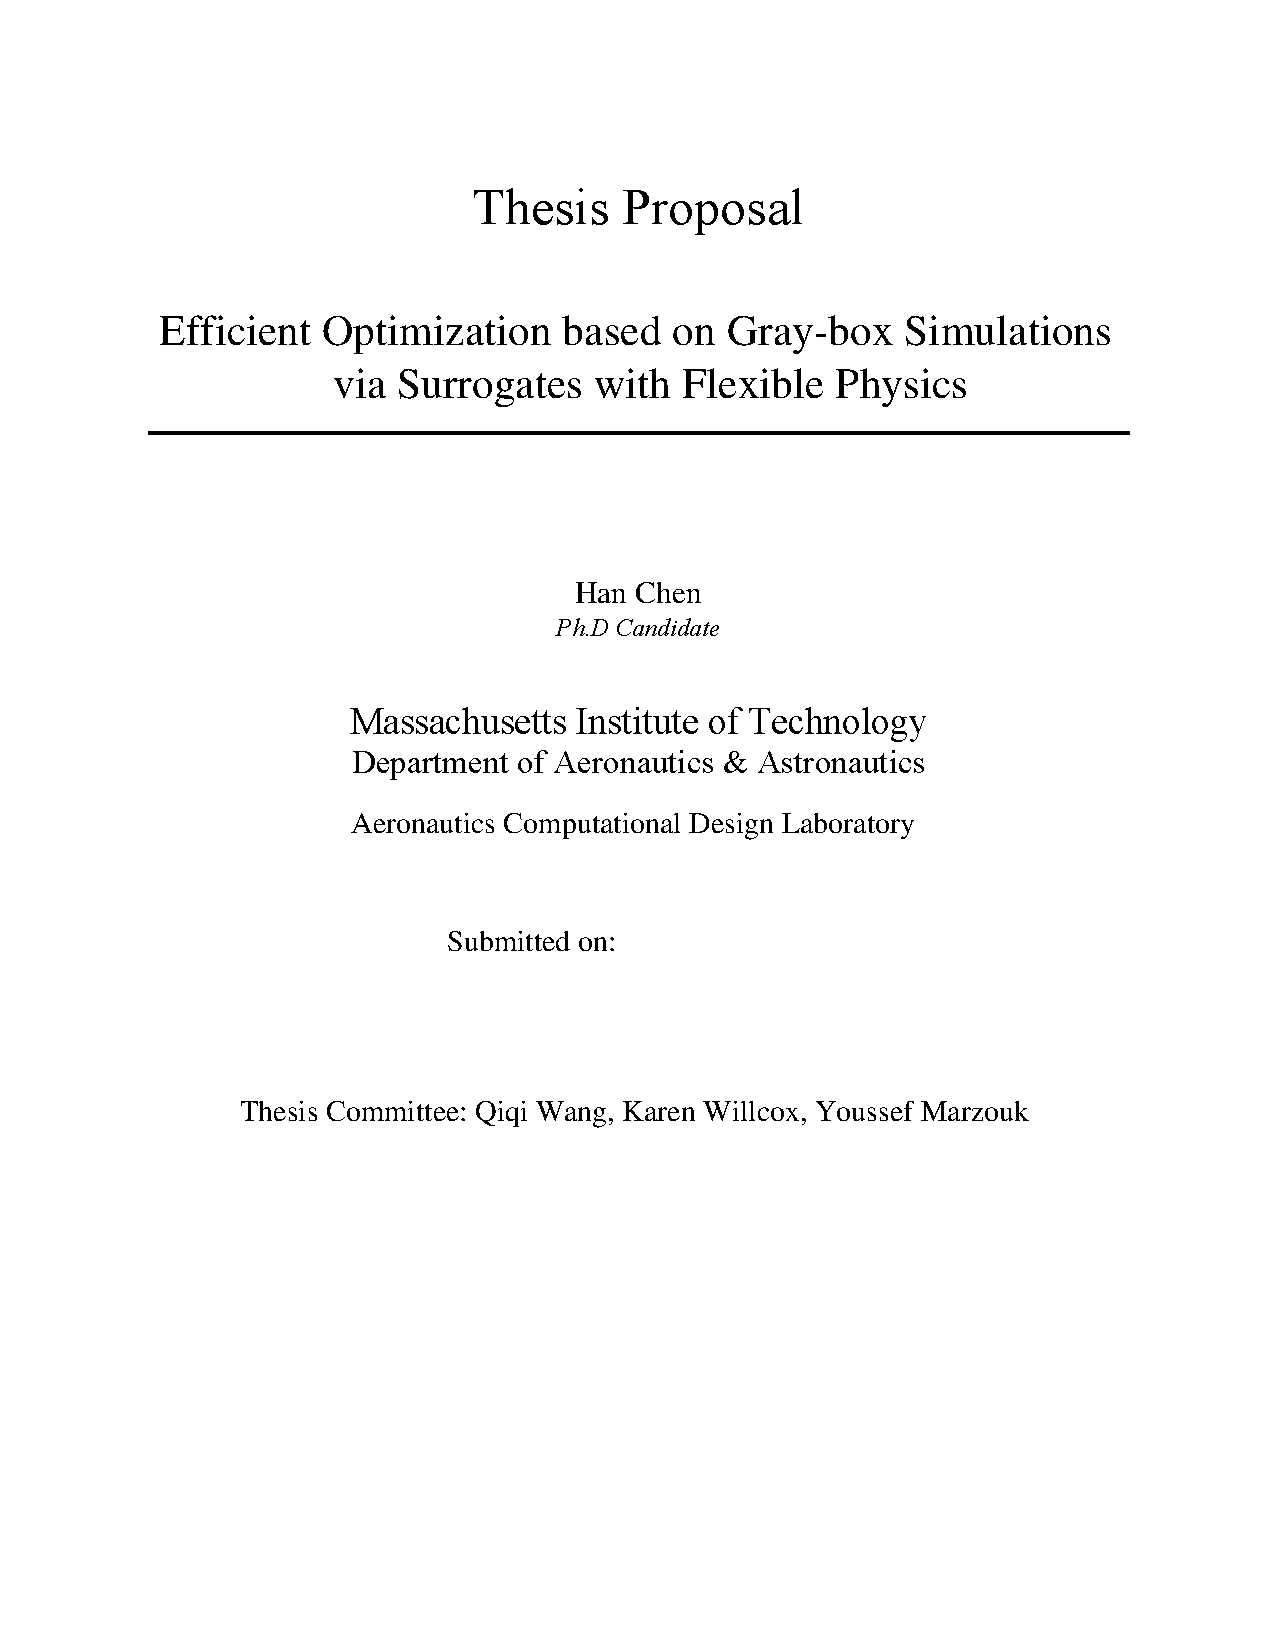
\includepdf[pages=-]{cover}
$$ $$
\newpage
\hspace{.4\textwidth}
\Large\textbf{Abstract}\\
\normalsize

\noindent Gray-box simulations of conservation laws are
present in many engineering applications. 
We call a conservation law simulation \emph{gray-box} if it can output the space 
(or space-time) solution of the flow-variables.
My thesis is interested in the optimization based on gray-box conservation law simulations,
which is a common task in the engineering community.
In many scenarios such simulations do not have adjoint implemented,
so we can not compute efficiently the gradients of 
the optimization's objective function with respect to the design variables. 
So conventional optimization practices generally treat the gray-box simulation
as only a calculator for the objective function. 
When the dimension of design space is high,
such conventional practices may require large amount of simulations which can be 
computationally prohibitive.\\

\noindent My thesis proposes an efficient methodology for
high-dimensional optimization problems by leveraging the limited insights
and the space or space-time solution of the gray-box simulation. 
My method constructs a PDE surrogate, 
called twin model, to serve as a low-fidelity avatar of the gray-box simulation. 
The innovation of my research is: the twin model mimics the gray-box simulation's space 
or space-time solution, instead of mimicing just the objective function.
The twin model first constructs a parameterized surrogate PDE, using the 
fact the gray-box simulation simulates a conservation law. Then it tunes the parameters to match the 
gray-box simulation's space or space-time solution.
Generally the space or space-time solution contains much more information 
about the gray-box simulation than the objective function.\\

\noindent Adjoint can be implemented in the twin model to 
estimate the gradient of the objective function with respect to design variables efficiently.
Optimization can be performed in a multi-fidelity framework using the low-fidelity
twin model and the high-fidelity gray-box simulation.
My thesis proposes a provably convergent Bayesian optimization scheme that combines
the evaluations of the gray-box' objective function with the twin model's gradient.
For completeness, we extend the optimization framework to constraint optimization.
\\

\noindent We propose to demonstrate our method by a turbulent flow optimization in a turbine airfoil
internal cooling problem. The gray-box
simulation is performed by a large eddy simulation (LES). 
The twin model is a Reynolds-averaged Navier-Stokes (RANS)
model with an adaptive Reynold stress. We optimize a return bend
geometry to minimize the pressure loss, and compare our result with state-of-art 
optimal designs.


\newpage
\tableofcontents


\newpage
\section{Background}
\label{intro}

\subsection{Optimization based on gray-box conservation laws}
Optimization problems is of great interest in the engineering community. We consider minimizing an
objective function:
$$
    J: \mathcal{C} \in \mathbb{R}^d\times [0,T] \rightarrow \mathbb{R}, \qquad c(t) \rightarrow J(c)\,,
$$
where $c(t) \in \mathbb{R}^d$ for $\forall t$. $c(t)$ is the design variable to be optimized.
In many cases, the objective function is an ouput of
a PDE based spatial-time simulation of conservation laws. 
For example, oil reservoir simulations may employ PDEs of the black-oil model, 
in which gas, water, and oil phases satisfy a set of conservation laws 
\cite{reservoir simulation book}. 
We may optimize the water injection logistics to maximize total oil production in a time window.
Another example is the DNS simulation for turbulent internal flow, in which mass, momentum, and energy
satisfy a set of conservation laws
\cite{Wilcox CFD}.
We may optimize the wall geometry to minimize the pressure loss.
The simulations employed for optimization are generally
implementations of PDEs for conservation laws, and can provide accurate predictions for 
the objective function.\\

\noindent In many cases, such simulations implement complicated PDEs and exotic solution techniques.
Besides, the PDEs and their numerical implementations may not
be accessible. For example, many industrial reservoir simulators are proprietary, such as \textit{Eclipse} (Schlumberger), 
\textit{VIP} (Halliburton), and \textit{PSim} (ConocoPhillips). During an internship in ConocoPhillips, 
I got a chance to
look at \textit{PSim}'s source code. It turns out to be a million-line, \textit{Fortran77}, legacy code developed for decades.
Therefore, even when the source code and the documentation are availble, it can still take tremendous amount of man power
to access, modify, and maintain the code.
When we have no insights of the PDEs or can not access its space-time solution,
the only duty of such simulations is to calculate the objective function
\begin{equation}
    J = J(c;\kappa) \in \mathbb{R}\,,
\end{equation}
where $\kappa\in \mathbb{R}^n$ are some pre-defined model properties (for example, porosity and permeability in oil reservoir simulation).
$c$ is the design variable to be optimized. 
We call such simulations \emph{black-box} \cite{review of black-box modeling}.\\

\noindent Fortunately, although it may be difficult to access the details of the PDEs, it's 
often easy to write down
the abstract form of the PDE. For example, many reservoir simulations can be written as \cite{reservoir simulation book}
\begin{equation}\begin{split}
    &\eta\frac{\partial u}{\partial t} + \nabla \cdot F(u, \kappa) = q(u,c)\\
    &J = \int_0^T\int_\Omega j(u,c) \; \textrm{d}t \textrm{d}\mathbf{x}\,,
\end{split}\end{equation}
with an impermeable reservoir boundary condition and known boundary conditions at well locations. 
$u\in \mathbb{R}^n$ includes field quantities like pressure and saturation. $\eta, \kappa\in \mathbb{R}^n$ 
are geology properties like porosity and permeability. $q\in \mathbb{R}^n$ is a known 
model for the volumetric change of $u$. 
$F\in \mathbb{R}^n$ is an unknown flux term. $c$ is the space-time-dependent design variable
such as water injection rates. Besides, many simulators can output the discretized $u(t,x)$ in addition to $J$.
For each evaluation of $J$ given $\kappa$ and $c$, the discretized space-time solution is generally 
a large file.
We will call such simulations \textit{gray-box}, 
in order to distinguish \textit{black-box} simulations where 
the space-time solution is unavailable.
Besides, in many cases, the simulations do not implement adjoint; we assume this property
to be shared by gray-box and black-box simulations. We will discuss the role of adjoint in more detail
in section \ref{gradfree_gradbased}.
If the PDE and its implementation are known, and if adjoint is implemented,
we call such simulations \emph{open-box}.
We summarize their differences in Table \ref{tab: boxes}.\\
\begin{center}
    \captionof{table}{Comparison of black-box, gray-box, and open-box simulations}
    \label{tab: boxes}
    \begin{tabular}{|c|c|c|c|c|}
        \hline
                   & PDE       & Implementation & {Space (or space-time) solution} & 
                   Adjoint\\ \hline
        Black-box  & \ding{56} & \ding{56}      & \ding{56}    & \ding{56}  \\ \hline
        Gray-box   & \ding{56}
                   & \ding{56}      & \ding{52}    & \ding{56}   \\ \hline
        Open-box   & \ding{52}      & \ding{52} &          &   \ding{52}      \\ \hline
    \end{tabular}
\end{center}

\noindent Thanks to the complicated physics models in the PDEs and large space-time scale involved, 
running a PDE-based simulation can be computationally expensive in many cases. 
In addition, optimization problems may entail a large number of 
PDE simulations, especially when the design space is high-dimensional.
Therefore, optimization based on PDE-simulations can be costly.\\

\noindent We will restrict our attention to optimization based on gray-box simulations with a high-dimensional design space.

\subsection{Prototypes for conservation laws and objective functions}
\label{psetup}
\noindent We will consider two prototypes of conservation laws governing the gray-box simulation: 
time-dependent and time-independent conservation laws.\\

\noindent For time-dependent conservation laws, the prototype is
\begin{equation}
    \frac{\partial}{\partial t}\left(\eta_i u_i\right) + \nabla \cdot 
    F_i(\mathcal{D} u, \kappa) 
    = q_i(u,c)\,, \qquad i=1,\cdots, n\,,
    \label{first equation}
\end{equation}
where $t\in[0,T]$ is time;
$x\in \Omega \subseteq \mathbb{R}^{n}$ is the spatial coordinate.
$\Omega$ may depend on the design $c$.
$q_i$'s are the source terms that may also depend on $c$.
$c$ is the design variable and may be space-time dependent.
The boundary and initial conditions are known. $F_i$'s are the flux functions. 
The flow variables are 
$u = \{u_1, \cdots, u_n\}$.
$\mathcal{D} u = \left\{u_1, \nabla u_1 , \cdots, \nabla^{i_1} u_1; \cdots;
u_n, \nabla u_n,\cdots, \nabla^{i_n} u_n\right\}$, where $\nabla^j$ indicates the $j$th
order spatial derivative tensor. We assume $i_1,\cdots, i_n$, i.e. the maximum 
order of derivatives, are known.
$\eta_i=\eta_i(x), \,\kappa=\kappa(x)$ are 
problem dependent spatial variables, and are assumed known. 
The discretized space-time solution of Eqn\eqref{first equation} given by a gray-box simulation
is written as $\hat{u}(t_i, \mathbf{x}_i; c)\,,\, i=1,\cdots,N$, where 
$t=\left\{t_1,\cdots, t_N\right\}$ indicates the discretized time, and 
$\mathbf{x}_i$ indicates the spatial discretization at time $t_i$.\\

\noindent The objective function is defined by
\begin{equation}
    J = \int_0^T \int_\Omega j(u,c) \textrm{d}\mathbf{x}\textrm{d}t
    \label{obj prototype}
\end{equation}
Notice $j$ can depend explicitly on c, while $u$ depends implicitly on $c$.
We will consider unconstraint optimization unless otherwise specified.\\

\noindent Similarly, for time-independent conservation laws, the prototype is
\begin{equation}
    \nabla \cdot 
    F_i(\mathcal{D} u, \kappa) 
    = q_i(u,c)\,, \qquad i=1,\cdots, n\,,
    \label{first equation steady}
\end{equation}
and the objective function is defined by
\begin{equation}
    J = \int_\Omega j(u,c) \textrm{d}\mathbf{x}
\end{equation}

\noindent Notice the time-independent prototype can be seens as a special case 
of the time-dependent prototype. In many cases, the solution of time-independent PDEs
can be seens as the converged solution of time-dependent PDEs. If we can evolve 
Eqn\eqref{first equation} until $\frac{\partial u_i}{\partial t}\rightarrow 0$,
the converged solution is a solution of Eqn\eqref{first equation steady}.
In numerical implementations, this corresponds to the pseudo time marching scheme
for solve time-independent PDEs. Therefore, we will mostly consider the time-dependent 
prototype.\\

\noindent For illustration purposes, 
consider an example for the time-dependent prototype. Consider 
a simulator modeling two phase flow in porous media.
One of the simplest yet classical model for two-phase porous media flow is the Buckley-Leverett model \cite{Buckley Leverett, Reservoir Simulation Book}. 
It models the displacement process of two-phase flow due to capillary pressure and Darcy's law.
The PDE, Buckley-Leverett equation, is
\begin{equation}
    \frac{\partial u}{\partial t} + \frac{\partial}{\partial x} \left(\frac{u^2}{1+A(1-u)^2}\right) = c\,,
    \label{Buck-Lev eqn}
\end{equation}
where $x\in[0,1]$ is the space domain;
$u = u(t,x)$, $0\le u\le 1$, is the saturation of phase I (e.g. water), 
and $1-u$ is the saturation of phase II (e.g. oil);
$A>0$ is a parameter dependent on the physical property of the two phases;
$c=c(t,x)$ is the design variable. $c>0$ models the injection of phase I replacing phase II; and $c<0$ vice versa.
Suppose $A$ is an unknown, we can use the prototype Eqn\eqref{first equation} to 
model the PDE.\\

\noindent As an example, we may
want to control the flow through $c$, such that the saturation at $t=T$ is close to 
a target saturation $u^*(x)$. We may introduce a Tikhonov regularization into the objective function 
to model the control cost \cite{Boyd optimization}.
Hereby the objective function
\begin{equation}\begin{split}
    J &= \int_x \left|u(T,x) - u^*(x)\right|^2 \textrm{d}x + \eta \int_t\int_x  c^2(t,x) \textrm{d}x\textrm{d}t\\
      &= \int_t \int_x \left|u(t,x) - u^*(x)\right|^2 \delta_T(t) + \eta c^2(t,x) \textrm{d}x \textrm{d}t \,,
\end{split} \label{BL objective}
\end{equation}
where $\eta>0$ models the price of control, and $\delta_\cdot(\cdot)$ is the Direc delta function.
Eqn\eqref{BL objective} can be modelled by Eqn\eqref{obj prototype}.
The optimization problem is
\begin{equation}
    c^* = \arg\min_{c\in \mathcal{C}} J
\end{equation}
where $\mathcal{C}$ can be the $L_2$-function Hilbert space.\\

\subsection{Gradient-free and gradient-based optimization}
\label{gradfree_gradbased}
\noindent Existing methods for optimization can be classed into two categories: 
using gradient information (gradient-based optimization) and not using gradient information (gradient-free optimization)
\cite{hanmaster, Opt Koziel Book}.
Gradient-free optimization methods require only the availability of objective function values but
not derivative information\cite{gradfreereview}. Because of its mild requirement of the simulation, 
gradient-free optimization methods are suitable for optimization problems based
on \textit{black-box}, \textit{gray-box}, and \textit{open-box} simulations, 
thus enjoy a wide range of applicability. However, when the dimension of the design space 
increases, these methods generally suffer from the \textit{curse of dimensionality}.
The term \textit{curse of dimensionality} refers to problems caused by the rapid increase in the search volume associated
with adding extra dimension in the search space\cite{dynamicprogramming}. It's not uncommon to encounter
tens or hundreds of dimensions in real life engineering problems, 
limiting the applicability of gradient-free optimization
in these cases.\\


\noindent Many strategies can be adopted to reduce the design space dimension 
\cite{survey of high dimensional blackbox optimization}, such as
dimensional reduction \cite{dimensional reduction}, system decomposition \cite{decomposition},
and variable selection \cite{variable selection}. However, these methods generally have 
additional assumptions or requirements to work properly \cite{survey of high dimensional blackbox 
optimization}. For example, some reduced order models reduce the design space
to a lower-dimensional subspace called \emph{active subspace} \cite{Han AIAA, Active subspace}.
Optimization may be performed only in the active subspace. 
For gray-box simulations, the active subspace can be estimated 
by sampling the relationship between the design variables and the objective function.  
However, when the original design space is high-dimensional, estimating the active subspace 
may still require an astronomical number of objective function evaluations. 
Some reduced order models consider the discretized-in-space ODE of the flow equations,
and reduces the dimension of the ODE using techniques such as proper 
orthogonal decomposition \cite{Balanced truncation}. But such methods require 
the ODE of the flow equations, which is not suitable under the gray-box assumption.\\

\noindent In contrast, gradient-based optimizations use gradient information to locate a local optimum.
A well-known example is the quasi Newton's methods \cite{quasiNewton}. 
Generally gradient-based methods require less number of simulations 
to converge than gradient-free methods, and are more efficient at finding local optimum for high-dimensional problems.
In addition of requiring $J(c)$ from the simulation,
these methods also require $\frac{\partial J}{\partial c}$, the sensitivity.
Adjoint methods are efficient methods for sensitivity analysis\cite{cont discretize adjoint}
for open-box models.
Continuous adjoint method develops the continuous adjoint equations from the continuous PDE of the simulation through 
Lagrange multiplier; and it requires the PDE of the simulation. 
Discrete adjoint method applies variational analysis directly to the discretized PDE; and it requires the
discretized PDE (i.e. the numerical implementation) of the simulation.
Another popular method to compute sensitivity is automatic differentiation (AD)\cite{automaticdiff}.
AD exploits the fact that every computer program can be broken down into a sequence of elementary arithmetic operations
and elementary functions. By applying the chain rule repeatedly to these operations, 
derivatives can be computed automatically. Because adjoint methods require
the accessibility of the PDE, and/or its implementation details, 
it can not be used to compute the sensitivity of a gray-box simulation either.\\

\noindent To sum up, gradient-free optimization methods are suitable for gray-box simulations, but suffer from the curse of
dimensionality; gradient-based optimization methods are more efficient for high-dimensional problems, but are not suitable for 
gray-box simulation. This dilemma motivates the development of a new optimization strategy. 
The new strategy should not require $\frac{dJ}{dc}$ from the gray-box simulation, 
and should be suitable for high-dimensional design space.\\

\subsection{Turbulent flow optimization}
\noindent Turbulent flow optimization may be a great playground to demonstrate
my proposed method.
There are many turbulence models ranging from low to high in terms of complexity and fidelity. 
Turbulence flow optimization generally considers objective functions of time averaged flow field. RANS model simulates a time averaged flow field directly, but the result can be inaccurate. Optimization based solely on high-fidelity simulations (e.g. LES, DNS) yields the most credible result. However, such optimization is computationally challenging. The challenge is two-folded: Firstly, these simulations generally require a tremendous amount of spatial-time discretization grid for sufficient resolution, and each objective function evaluation can be both lengthy in time and costly in computational resources. Secondly, these high-fidelity simulators generally do not have adjoint capability; so estimations of the gradient, a key to efficient optimization, is difficult to obtain especially for high dimensional design space.\\

\noindent LES is a popular high-fidelity turbulent flow model. Generally LES simulations 
can be considered gray-box. 
Firstly, LES models a chaotic dynamical systems. 
It is not trivial to obtain the correct adjoint sensitivity \cite{chaotic Qiqi}.
Secondly, LES employs a large number of space-time grid points, thus it can be CPU and memory
expensive to implement the adjoint.
Thirdly, LES may involve exotic boundary conditions, so the PDE and their implementations
may not be easily accessible
to engineers who are not experts in computational fluid dynamics.
Fourthly, LES simulators can produce the space-time solution of all relevant flow fields
such as velocity and pressure.\\

\noindent Low-fidelity simulations such as steady RANS can be open-box. 
Steady RANS solves a time-independent problem for the mean flow field.
They are generally much cheaper to solve, and easier to implement adjoint. However,
they may have worse accuracy than the high-fidelity simulations.\\

\noindent We consider optimization problems based on turbulent flow simulation. 
When the design space is low, optimization can be performed directly with high-fidelity optimization
\cite{Chai opt}. For higher dimensional design space, the state-of-art optimizations can
only employ low-fidelity models such as RANS. However, there is no guarantee for
the low-fidelity model's optimum to be close to the high-fidelity model's optimum.
Multifidelity optimization may be applied to turbulence optimization. 
However, low-fidelity models may not be good representation of high-fidelity models, thus limiting computational savings. \\


\newpage
\section{Thesis objective, expected contribution, proposed schedule}

\subsection{Thesis objective}
\begin{enumerate}
    \item Develop a method for inferring a surrogate conservation law 
    from the space or space-time solution of an unknown conservation law's PDE simulation.
    \item Assess how much computational saving can be achieved using
    the proposed framework in a return bend optimization problem.
\end{enumerate}

\subsection{Expected contribution}
\begin{enumerate}
    \item Enable adjoint gradient computation even if the governing PDE is not available.
    \item Demonstrate that efficient gradient-based optimization is possible, even if the underlying simulator does not implement
          an adjoint.
    \item Demonstrate my method's superiority in a high-fidelity turbulent flow optimization with a
    high-dimensional design space.
\end{enumerate}


\subsection{Proposed schedule}
\noindent \textbf{Completed:}
\begin{itemize}
    \item Course work.
    \item Formulation of twin model and its inference.
    \item Basis selection for time-dependent twin model.
    \item Optimization framework using twin model.
    \item Demonstration of twin model in a 1D example.
\end{itemize}
\noindent \textbf{To be complete:}
\begin{itemize}
    \item \textbf{2015 Apr}: Write proposal defense slides. Wrap up the proof of theorem \ref{theorem: 2}.
    \item \textbf{2015 May}: Defend proposal. Demonstrate the complete algorithm on a the 1D Buckley-Leverett example.
    \item \textbf{2015 Jun}: Setup an LES solver for the return bend testcase in OpenFoam, write a RANS solver with adjoint for the return bend.
    \item \textbf{2015 Jul}: Hold a committee meeting for progress report.
    \item \textbf{2015 Jul-Oct}: Implement optimization on the return bend example.
    \item \textbf{2015 Aug-Nov}: Write thesis.
    \item \textbf{2016 Jan}: Defend thesis.
\end{itemize}

\newpage
\section{Twin model}
\label{gradient_surrogate}
\subsection{Review of surrogate methods}
\label{review surrogate methods}
\noindent As mentioned in chapter \ref{intro}, 
straightforward optimization of $J(c)$ using gray-box simulations
is not always practical.
A well-studied topic to address this problem is \emph{surrogate-based optimization}
\cite{Opt Koziel Book, Surrogate based analysis and optimization}.
It is proposed to achieve optimization at reduced computational cost \cite{Space mapping 1}.
A \emph{surrogate} gives a reasonably accurate representation of the high-fidelity model's $J(c)$.
We will call the high-fidelity gray-box simulation
the \emph{primal model}, and write its objective function as $J(c)$;
we will write the surrogate model's objective function as $\tilde{J}(c)$.
In surrogate-based optimization, the optimization using the primal model can be
replaced by iteratively updating and re-optimizing the surrogate.
The design point generated by optimizing the surrogate is verified by evaluating
the primal model. The primal model evaluation is then used to update/correct the surrogate.
Surrogate-based optimization generally proceeds in this prediction-correction manner until
termination.\\

\noindent Surrogate-based optimization methods can be distinguished by how the surrogate is 
constructed. Surrogate construction techniques can be categorized into
\emph{physics-based surrogate} and \emph{functional surrogate} \cite{Opt Koziel Book}.
Similar to the primal model, physics-based surrogate simulates the underlying physics.
The surrogate is still a representation of the underlying system's physics, but has 
lower fidelity and is cheaper to evaluate: generally because it
uses simplified physics \cite{simplified physics, Space mapping 1} and/or
uses coarse discretization \cite{coarse discretization}. For example, reduced order
models based on balanced truncation \cite{Balanced truncation} can be viewed as 
a physics surrogate, where a reduced dimensional ODE derived from the original 
ODE is used to describe the system dynamics.
A functional surrogate, on the other hand, are generally constructed using only the sample
values of $J(c)$ obtained from the primal model (and gradient of $J(c)$ if
the primal model can also evaluate the gradient \cite{gradient kriging surrogate}).
Functional surrogate does not require insights of the dynamics of the system. 
Popular functional surrogate techniques include polynomial approximation 
\cite{poly functional surrogate}, Kriging \cite{kriging functional surrogate},
artificial neural network \cite{ann functional surrogate}, etc.\\

\noindent Generally, physics-based surrogates are more expensive to evaluate but more accurate,
mainly because they already embed some knowledge of the system's physics. 
However, physics-based surrogates are dedicated to the specific systems of interest.
The construction of physics-based surrogates often require expert insights
and significant coding manpower \cite{Opt Koziel Book}. 
Functional surrogates, on the other hand, are generic to a wide class of problems.
The price paid is they may require considerable amount of primal model evaluation 
to achieve the same accuracy as physics-based surrogates. \\

\noindent Designing a good physics-based surrogate requires expert insight
(e.g. the choice of empirical formulas or the negligence of unimportant physics components),
thus limits its applicability. Besides,
many physics-based surrogates are only good approximations of the primal model
within a certain range of physics settings. 
For example, the thin airfoil theory is only valid before stall. 
If one is to optimize the attack angle, the thin airfoil models may no longer 
provide good estimation of the primal model when the attack angle increases \cite{thin airfoil}.
Another example is from turbulent modelling.
Some simplified fluid models are derived under the assumption of low Reynolds number
\cite{turbulent modeling R low}, while some are derived under high Reynolds number 
\cite{turbulent modeling R high}.
In optimization, however, design variables 
move at each iteration. A low-fidelity model may gradually lose its accuracy 
as the design variables move away from the surrogate's applicable region.
If one is to optimize the attack angle using a surrogate of thin airfoil theory, 
or optimize the flow speed using a low or high Reynolds number fluid model, 
the quality of the optimum can be questionable.\\

\noindent To alleviate the drawbacks in surrogates, 
there have been many researches to \emph{correct} the surrogate's objective function
iteratively online to improve its accuracy. Generally, existing methods
use $J(c)$ to correct the surrogate's $\tilde{J}(c)$.
One method is \emph{Bayesian model calibration}
\cite{KennedyOhagan1, andrewras}. This method models the error,
$J(c) - \tilde{J}(c)$, as a deterministic but unknown  
realization of a stochastic process.
It infers the error at unsampled $c$ via a Bayesian framework,
using existing samples of $J(c)$ and $\tilde{J}(c)$.
The inferred error is then added to $\tilde{J}(c)$ to provide a corrected surrogate.
Another method is \emph{multi-fidelity trust-region method}, i.e. to bound the search step
inside a \emph{trust region} during each optimization iteration \cite{trustregionwild}.
The surrogate is corrected to guarantee good estimation
of the primal model within a trust region
(e.g. satisfying the \emph{fully-linear} property \cite{trustregionconn}),
before performing optimization using the surrogate within the trust region.\\

\noindent These research efforts (Bayesian model calibration, multi-fidelity 
trust-region methods, etc) can be viewed as overlaying the existing surrogate model with 
an additional \emph{functional}
surrogate for correction. In order for the correction to improve the existing surrogate 
to a desirable accuracy, a large number of primal model evaluations may be required.
This is a common problem suffered by functional surrogate.\\

%\noindent To sum up, physics-based surrogates have two drawbacks:
%1. They require expert knowledge for construction. 2. Their physics are fixed offline
%and may not always give good approximations during optimization.\\

\subsection{Infer physics-based surrogate by the space-time solution}

\noindent The problem roots in using $J(c)$ to correct a functional surrogate. 
For a single-objective optimization problem, each high-fidelity simulation yields
only a single $J(c)$ to correct the surrogate. When the design space is high, the
correction is clearly inefficient.\\

\noindent As we mentioned earlier, many research efforts can be viewed as overlaying an
existing surrogate with an additional functional surrogate.
Instead, we may infer an adaptive physics-based surrogate, where
the physics of the surrogate is adaptive. 
In other words, the physics-surrogate can morph its representation of the 
underlying system's physics on-the-fly, so as to better represent the primal model for
a wider range of physics settings.
According to our gray-box assumptions in chapter \ref{intro},
the only knowledges available in adapting the physics-based surrogate
are the sampled $J(c)$'s and corresponding space-time solutions $u(t,x;c)$'s.\\

\noindent Is it feasible to infer a
physics-based surrogate? Consider a general dynamical system
\begin{equation}
    \dot{u} = \mathcal{L}(u)\,,
    \label{general equation}
\end{equation}
where $u=\{u_1,\cdots, u_n\}$, $u_i = u_i(t,x)$, $i=1,\cdots,n$, $x\in \mathbb{R}^n$.
$\mathcal{L}$ is a differential operator known as the Hamiltonian of the system 
\cite{Hamilton Fluid Dynamics}.
Suppose an observer can take snapshots of $u$ at any $t$.
It has been shown that inferring $\mathcal{L}$ from the snapshots is an intractable
problem, no matter how many snapshots are observed \cite{NP hard}.
Although Eqn\eqref{general equation} offers the most general description of the 
primal model, we may not be able to infer a physics-based surrogate 
just based on Eqn\eqref{general equation}.\\

\noindent However, inferring the differential operator $\mathcal{L}$ 
is not necessary. As discussed in
chapter \ref{intro}, 
the PDEs for the conservation laws can be written as prototypes Eqn\eqref{first equation}
or Eqn\eqref{first equation steady}.
Therefore, the problem of adapting the physics of the physics-based surrogate reduces to the
problem of adjusting a set of functions $F_i$ or
$q_i$, for $i=1,\cdots,n$. \\

%In addition, we can use the discretized space-time solution 
%$\hat{u}(t_i,\mathbf{x}_i;c)$, provided by the primal model, to adjust the 
%physics of twin model.
%$\hat{u}(t_i,\mathbf{x}_i;c)$ is a by-product of evaluating $J(c)$,
%but provides more information than $J(c)$ about the underlying system's physics
%\cite{hanmaster}.
%Finally, as we write the twin model in a conservative form, 
%the implementation of twin model can be guaranteed to conform to conservation laws
%using appropriate numerical schemes such as finite volume methods
%\cite{numerical schemes for hyperbolic equation review}.\\


\noindent We \textbf{use the space-time solution} of the gray-box simulations 
to infer these functions.
There are several benefits to use the space-time solution \cite{hanmaster}.
Firstly, in conservation law simulations, the flow quantities only depend on the flow
quantities in an older time inside a \emph{domain of dependence}.
When the timestep is small,
the domain of dependence can be small too. For example, for scalar conservation laws 
without exogenous control,
we can view solving the conservation law for one timestep $\Delta t$ as a mapping 
$\mathbb{R}^{\omega_{\Delta t}} \rightarrow \mathbb{R}$, where $\omega_{\Delta t}\in \Omega$ 
is the domain of dependence. 
Loosely speaking, by applying such mapping repeatedly to all $x\in \Omega$ and $t\in[0,T]$
(in addition to the boundary and initial conditions), we perform 
a space-time simulation of the conservation law. 
Generally, the size of $\omega_{\Delta t}$ is small.
Therefore, in the discretized simulation of conservation laws,
the number of discretized flow variables involved in $\omega_{\Delta t}$ is small too,
making it feasible to infer the mapping.
In my master thesis, such a property is termed \emph{stencil locality} \cite{hanmaster}.
\\

\begin{figure}[H]\begin{center}
    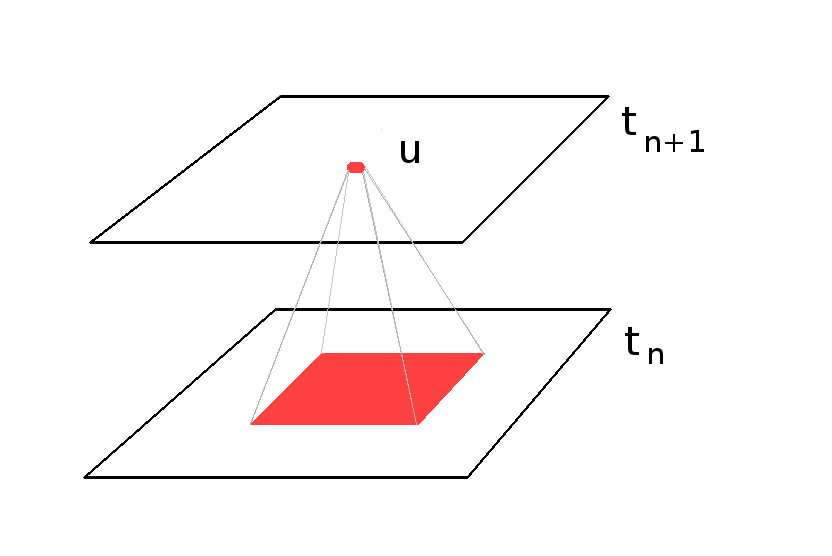
\includegraphics[height=5cm]{locality.png}
    \caption{Domain of dependence: in conservation law simulations,
             the flow quantities at a given location
             depends on the flow quantities at an older time only within its
             domain of dependence $\omega$. The domain of dependence can be much smaller
             then the overall spatial domain $\Omega$ when the timestep is reasonably small.}
    \label{locality}
\end{center}\end{figure}

\noindent Secondly, the space-time solution at almost \emph{every} space-time grid point can be viewed
as a sample for the mapping $\mathbb{R}^\omega \rightarrow \mathbb{R}$. 
Because the number of space-time grid points in gray-box simulations is generally large,
we have a large number of samples to infer the mapping. 
In the prototype PDEs Eqn\eqref{first equation} and Eqn\eqref{first equation steady},
such a mapping is determined by the functions $F_i$'s or $q_i$'s.
Therefore, we will have a large number of samples to infer the functions,
making the inference potentially accurrate.
In my master thesis,
such a property is termed \emph{physics invariance} \cite{hanmaster}.\\

\noindent Thirdly, in many optimization problems, the design space is high only because
the design is space and/or time dependent. In order to parameterize the space-time dependent
design, a large number of design variables will be employed. However, 
the flow quantities only depend on the design variables in the domain of dependence.
Therefore, even if the overall number of design variables is high, the number of design variables
involved in the mapping is limited, making the inference problem potentially
immune to the design space dimensionality.\\

\noindent Therefore, we propose to infer a new type of surrogate using 
the prototype equations Eqn\eqref{first equation} or
Eqn\eqref{first equation steady} and the space-time solution of the gray-box simulation.
The proposed surrogate is called \emph{twin model}.

%In the mean time, the \emph{physics} of the physics-based surrogate is still fixed offline
%before the optimization. Can we use primal model samplings to
%directly correct the physics of the surrogate? Bearing this question at mind,
%we propose \emph{twin model}: a physics-based surrogate model with flexible physics.\\


\subsection{Twin model as an inverse problem}
\label{inverse}
\noindent 
Conventionally, we have a given PDE, and want to compute
its space-time solution. However, in twin model we want to infer the governing PDE
to match a given space-time solution.
Finding a suitable prototype equation can be viewed
as an inverse problem. Inverse problems typically involve the estimation of certain variables
based on indirect measurements of these quantities. In the theory of inverse problems,
a model that computes the indirect
measurement given the estimation variables is called a \emph{forward model}.
If we parameterize the functions $F_i$'s or $q_i$'s in the prototype equations,
we get an inverse problem of estimating such parameters.
\\

\noindent Methods for solving inverse problems can be classed into two categories:
statistical estimation and parameter identification. 
Statistical estimation methods
adopts a statistical description of the estimation variables. Generally
the measurement is assumed noisy, with the noise described by a probability measure.
By computing the likelihood of the measurements given the estimation variables,
Bayesian inference can be performed to obtain a point estimate or a probability description
of the estimation variables \cite{inverse book}. Such methods generally keep track of an ensemble of 
estimation variables. In our problem, this is equivalent to maintain an ensemble of
twin models with different function $F_i$'s or $q_i$'s.
Because each twin model is itself
a PDE simulator; it can be expensive to maintain such an ensemble. 
In addition, it may be inappropriate to model the gray-box simulation's space-time solution as noisy.\\

\noindent Another category is parameter identification. Parameter identification
infers the estimation variables from a measurement, so the measurement computed 
from the forward model and the actual measurement can match
\cite{inverse book}.
Loosely speaking, in twin model
we infer the prototype equations so that a metric of the space-time solution mismatch is minimized.
The metric is to be determined.
Parameter identification treats the estimation variables deterministically. 
Gradient-based optimization can be used in parameter identification to efficiently
infer the optimal estimation variables. We will employ parameter estimation to infer
the twin model.\\

\noindent Twin model is an open-box. Therefore, adjoint method 
can be implemented for efficient parameter identification.
Let
the flow variables solved by the twin model be $\tilde{u}$,
the flow variables given by the gray-box simulation be $u$,
the metric of the space-time solution mismatch be $L(u,\tilde{u})$,
the variables parameterizing the twin model be $\xi$,
and the forward model be $\tilde{R}(\tilde{u},\xi) = 0$.
Adjoint method proceeds by linearizing $L$ and $\tilde{R}$,
\begin{equation}
    \delta L = \left(\frac{\partial L}{\partial \tilde{u}}\right)^T \delta \tilde{u}
\end{equation}
\begin{equation}
    \frac{\partial \tilde{R}}{\partial \tilde{u}} \delta \tilde{u}
    + \frac{\partial \tilde{R}}{\partial \xi} \delta \xi = 0
\end{equation}
Introduce a Lagrange multiplier $\lambda$, a.k.a. \emph{adjoint state}, we have
\begin{equation}\begin{split}
    \delta L &= \left(\frac{\partial L}{\partial \tilde{u}}\right)^T \delta \tilde{u}
    - \lambda^T \left(\frac{\partial \tilde{R}}{\partial \tilde{u}} \delta \tilde{u}
    + \frac{\partial \tilde{R}}{\partial \xi}\delta \xi\right)\\
    &= -\left( \lambda^T \frac{\partial \tilde{R}}{\partial \xi}\right) \delta \xi
    + \left( \left(\frac{\partial L}{\partial \tilde{u}}\right)^T 
        - \lambda^T \frac{\partial \tilde{R}}{\partial \tilde{u}}
    \right)\delta \tilde{u}
\end{split}\end{equation}
Therefore, the adjoint state satisfies the \emph{adjoint equation}
\begin{equation}
    \left(\frac{\partial \tilde{R}}{\partial \tilde{u}}\right)^T \lambda 
    = \frac{\partial L}{\partial\tilde{u}}\,,
\end{equation}
and the gradient is given by
\begin{equation}
    \frac{\partial L}{\partial \xi} = -
    \left(\frac{\partial \tilde{R}}{\partial \xi}\right)^T \lambda
\end{equation}



%\subsection{Review of system identification}
%\label{SI review}
%\noindent The inference problem can be viewed as a \emph{system identification} problem. 
%System identification is
%a method that builds mathematical models of a
%dynamical system from its measured data \cite{SI old}.
%System identification generally considers experimental data. However, 
%its concepts are also applicable to the data generated by gray-box simulations.
%Specifically, we want to identify the prototype equations using the space-time solution
%of the gray-box simulations.\\
%
%\noindent Depending on the how the system is modelled, system identification 
%can be classified into \emph{linear system identification} and
%\emph{nonlinear system identification}. Linear system identification assumes a linear
%relationship between the system inputs $\mathbf{x}(t)$ and output $y(t)$:
%\begin{equation}
%    y(t) = h_0 + \sum_{i=1}^n \int_0^t h_i(\tau) x_i(t-\tau) \, d\tau
%    \label{linear dynamic}
%\end{equation}
%The advantage is a linear model can be determined solely by its
%impulse response function.
%Clearly, the twin model
%is generally nonlinear and may not be modelled well by a linear system.
%Nonlinear system identification does not assume this linearity, thus is more generic
%\cite{NARMAXbook}.
%We will restrict our attention to nonlinear system identification.\\
%
%\noindent Well-known models for nonlinear system identification include
%\cite{NARMAXbook}: \emph{piecewise linear models},
%\emph{block-structured models}, 
%\emph{Volterra models}, and \emph{NARMAX} models. 
%A piecewise linear model develops a series of locally linear approximations
%to the system. In our problem, this model would adopt a piecewise linear 
%representation of $F_i$'s and $q_i$'s. 
%This approach can utilize the wealth of knowledge obtained from the research in linear systems.
%But a drawback is the difficulty to partition the parameter domain, because
%the estimation of piecewise model can not be easily separated from the task of finding the
%domain for each sub-model \cite{piecewise linear}.\\
%
%\noindent Block-structured models are described by connections of groups of linear 
%and nonlinear models \cite{NARMAXbook}.
%For example, Hammerstein model applies a nonlinear scaling of the input before transmitting
%it to a linear dynamic model described by Eqn\eqref{linear dynamic}.
%Wienner model, on the other hand, applies the nonlinear scaling after the dynamic model.
%\begin{figure}[H]\begin{center}
%    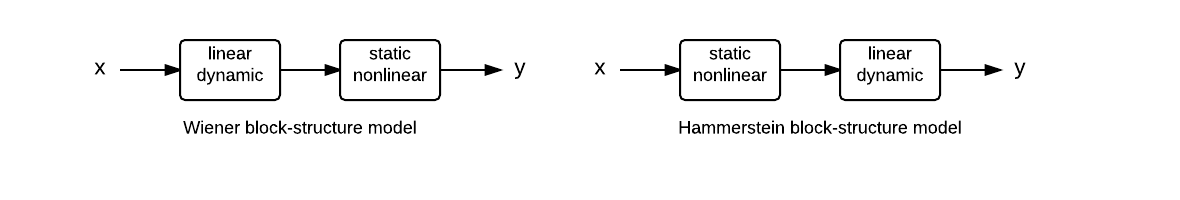
\includegraphics[height=2.5cm]{blockstructure.png}
%    \caption{block structure model}
%\end{center} \label{Wiener}
%\end{figure}
%\vspace{-.5cm}
%\noindent 
%These models became popular after theoretical results showing a nonlinear scaling operation 
%preserves the cross variance of Gaussian stochastic signals \cite{cross correlation}. 
%Another type of block-structured models are feedback linear models, in which the output
%of the linear dynamic model is feed to its input \cite{feedback linear}.
%\begin{figure}[H]\begin{center}
%    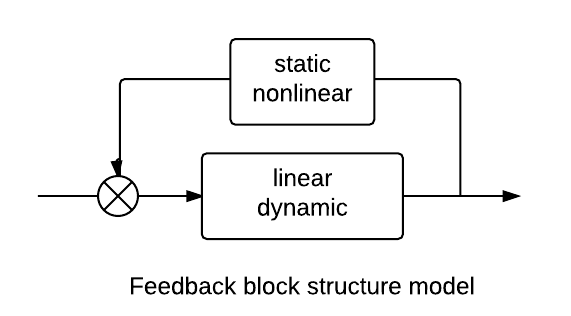
\includegraphics[height=3cm]{feedback.png}
%    \caption{feedback model}
%\end{center} \label{Wiener}
%\end{figure}
%\vspace{-.5cm}
%\noindent 
%However, almost all these methods rely on previous knowledge that the system under study
%has a specific structure \cite{NARMAXbook}. Besides,
%most researches on block-structured models focus on SISO, MISO, and MIMO systems,
%instead of PDE systems.
%They directly model the transformation from the system input to the
%system output, failing to take advantage of the PDE form expressed by Eqn\eqref{first equation}. 
%Indeed, block-structured models may overly restrict the form of the model.
%We would prefer a more general description of the model.
%\\
%
%\noindent Volterra models, a.k.a. Volterra series models, use polynomials to represent 
%the system. It is similar to a Taylor series but has a memory effect \cite{volterra 1, volterra 2}.
%If we think of Taylor series as a functional that applies to a snapshot of $u(x,t)$ for
%a fixed $t$, then the Volterra series can be thought as a functional that applies to
%the whole history of $u(x,t)$ \cite{NARMAXbook}.
%We call a Volterra model of $k$th order if the polynomial is of $k$th order.
%For example, if $F = F(x(t))$, then an $m$th order Volterra model on
%$t\in [0,T]$
%would approximate $F$ as
%\begin{equation}\begin{split}
%    F &\approx h_0 + \sum_{k=1}^m H_k x(t)\\
%    H_k x(t) &= \int_{\tau_1=0}^T \cdots \int_{\tau_k=0}^T 
%    h_k(\tau_1, \cdots, \tau_k) \prod_{j=1}^k x(t-\tau_j) d\tau_j
%\end{split}\end{equation}
%More generally, for $F = F(x_1(t),\cdots, x_n(t))$, an $m$th order Volterra model would be
%\cite{volterra 1}
%\begin{equation}\begin{split}
%    F & \approx h_0 + \sum_{p=1}^m H_p \mathbf{x}(t)\\
%    H_p \mathbf{x}(t) &= \sum_{
%        \begin{split}
%           & \scriptscriptstyle k_1\ge 0,\cdots,k_n\ge 0\\[-2.3mm]
%           & \scriptscriptstyle k_1+\cdots+k_n=p
%        \end{split}
%    }
%    \int_{\tau_{j_1}} \cdots \int_{\tau_{j_n}} 
%    \prod_{j_1=1}^{k_1} \cdots \prod_{j_n=1}^{k_n}
%    h_{k_1,\cdots,k_n}(\tau_{j_1}, \cdots, \tau_{j_n})
%    x_1(t-\tau_{j_1}) d\tau_{j_1}\, \cdots\,
%    x_n(t-\tau_{j_n}) d\tau_{j_n}
%\end{split}\end{equation}
%A special case of Volterra model is a \emph{memoryless} polynomial expansion, written as
%\begin{equation}
%    H_p \mathbf{x}(t)= \sum_{
%        \begin{split}
%           & \scriptscriptstyle k_1\ge 0,\cdots,k_n \ge 0\\[-2.3mm]
%           & \scriptscriptstyle k_1+\cdots+k_n=p
%        \end{split}
%    }
%    h_{k_1,\cdots,k_n}
%    x_1^{k_1}(t) \cdots x_n^{k_n}(t)
%    \label{polynomial Volterra}
%\end{equation}
%As discussed in section \ref{psetup}, our unknown flux function
%$F_i$ only depends on \\
%$\mathcal{D}u = \left\{u_1, \nabla u_1 , \cdots, \nabla^{i_1} u_1; \cdots;
%u_n, \nabla u_n,\cdots, \nabla^{i_n} u_n\right\}$, rather than depending on the time history of $u$.
%Therefore Eqn\eqref{polynomial Volterra} suffices to describe the unknown flux.\\
%
%\noindent NARMAX models (nonlinear autoregressive moving average models with exogeneous parameters),
%introduced in \cite{billings 1981}, provides a more general model description.
%Initially it was invented to model a \emph{discrete} SISO system with exogeneous inputs $\mathbf{u}$
%and output noise $\mathbf{e}$:
%\begin{equation}
%    y(t) = F[y(t-1), y(t-2), \cdots, y(t-n_y), u(t-1), u(t-2),\cdots, u(t-n_u),
%    e(t-1), e(t-2), \cdots, e(t-n_e)] + e(t)
%\end{equation}
%Hereby NARMAX' name.
%While NARMAX started as the name of a model, it has now developed into a philosophy of 
%nonlinear system identification.
%The philosophy consists of the following steps to identify a model \cite{NARMAXbook}:
%\begin{itemize}
%    \item \emph{Model representation}:  Represent $F$ by a library of terms
%    \item \emph{Structure detection}:   Remove unnecessary terms in the expansion
%    \item \emph{Parameter estimation}:  Fit the term coefficients
%    \item \emph{Model validation}:      Check if the model's error is predictable
%\end{itemize}
%The first step is to expand the functional form $F$ by a \emph{linear} combination
%of a library of \emph{basis} terms;
%for example, using Volterra series models, wavelet decomposition \cite{Wavelet SI}, 
%neural networks \cite{ANN SI}, etc. The choice of the library is up to the user's
%choice. 
%However, a naive proceeding to fitting the coefficients of all the terms in the library
%can be computationally intractable.
%Often there are only a few terms in the library that are important in the model.
%So the next step is to detect those terms. 
%NARMAX proceeds this step by first selecting the most important term, then
%the next most important terms, and so on, until a termination criterion is met. We'll investigate
%the structure detection step in greater detail in section \ref{adaptive}.
%After the structure detection, NARMAX estimates the coefficients of the terms, for example using
%a mean square error approach, so the output of the identified model and the 
%underlying system match on the sampled inputs.
%Finally, the model is validated to check if the identified model
%is adequate, for example, if there is anything
%predictable left in the model output's error \cite{correlation model validation}. 
%Unless the model is determined adequate, the term library will be enlarged and the previous 
%procedures will be conducted again.
%We'll discuss the model validation step in section \ref{future work}.\\
%
%\noindent 
%We will adopt the NARMAX philosophy to identify the twin model because of two considerations.
%Firstly, NARMAX is generic.
%It does not pose any limitation on the model representation library beforehand.
%Secondly, NARMAX is parsimonious.
%It attempts to find the simplest model structure before fitting the term coefficients.
%In my thesis,
%we will expand the functionals $F_i$'s in Eqn\eqref{first equation}
%by a library of terms.  The choices of the library will be explored.
%Then we will use NARMAX philosophy to fit the $F_i$'s.
%Chapter \ref{gradient_surrogate} will discuss fitting the twin model without the structure 
%detection step, i.e. twin model with fixed structure.
%Chapter \ref{adaptive} will focus on the structure detection.\\

\subsection{Formulation of twin model's inference}
\label{general formulation}
\noindent In the parameter identification,
we need a metric for the mismatch of the space-time solutions.
Given the same inputs (design variables, initial conditions, boundary conditions, and exogenous 
inputs), an ideal twin model should give a space-time solution $\tilde{u}$ such that
\begin{equation}
    \frac{1}{T}
    \int_{t=0}^T\int_{\mathbf{x}\in\Omega} w^2(t,\mathbf{x}, u,\tilde{u}) (\tilde{u} - 
    u)^2 \, dtd\mathbf{x}\,,
    \label{minimizer twin model}
\end{equation}
is minimized,
where $w^2>0$ is a weight possibly depending on $t$, $\mathbf{x}$, $u$, and $\tilde{u}$.
We will delay the discussion of $w$ to section \ref{future work}.
Right now we assume $w\equiv 1$ for simplicity.
Notice the square on $\tilde{u}-u$: it is a differentiable expression
whose derivative is smooth.\\

\noindent The space-time solution is discretized rather than continuous. 
If the twin model and the 
primal model use the same space-time grid, then Eqn\eqref{minimizer twin model} can be
approximated by
\begin{equation}
    \frac{1}{T}
    \sum_{i=1}^{N}\sum_{k=1}^{T} \left(\tilde{u}_{ik} - u_{ik}\right)^2 \Delta t_k
    \left| \Delta \mathbf{x}_i \right|\,,
    \label{minimizer twin model discrete}
\end{equation}
where $\left| \Delta \mathbf{x}_i \right|$ indicates the size of the grid.
If the grids are different, then a mapping $P$ from $u$ to $\tilde{u}$ is required.
In this case, Eqn\eqref{minimizer twin model discrete} would translate to
\begin{equation}
    \frac{1}{T}
    \sum_{i=1}^{N}\sum_{k=1}^{T} \left(\tilde{u}_{ik} - P(u)_{ik}\right)^2 \Delta t_k
    \left| \Delta \mathbf{x}_i \right|\,,
    \label{minimizer twin model discrete mapping}
\end{equation}
Right now, we assume the grids are the same for simplicity.\\

\noindent 
In the following we assume $F_i$'s are unknown in the prototype equations
(the extension to problems with unknown $q_i$'s
is straightforward). By parameterizing the functions using a set of basis,
the problem of constructing a twin model
is converted to the following problem. Notice we added a Tikhonov regularization
to avoid ill-posedness. \\

\fbox{\parbox{\textwidth}{
Solve
\begin{equation}
    \xi^* = \arg\min_{\xi} L(\tilde{u}(\xi)) =
    \arg\min_{\xi} \left\{
    \frac{1}{T}
    \sum_{i=1}^{N}\sum_{k=1}^{T} \left(\tilde{u}_{ik} - u_{ik}\right)^2 \Delta t_k
    \left| \Delta \mathbf{x}_i \right|
    + \lambda \|\xi\|^2  \right\}
    \,,
    \label{objective twin model}
\end{equation}
where $u$ is the discretized space-time solution of the primal model, and $\tilde{u}$
is the discretized space-time solution of
\begin{equation}
    \frac{\partial\eta_s \tilde{u}_s(t,x)}{\partial t} + \nabla \cdot \left\{
    \sum_{k=1}^{m_s}\xi_{sk} g_{sk}(\mathcal{D} \tilde{u}, \kappa)  \right\}
    = q_s(\tilde{u},c(t,x))\,, \qquad s=1,\cdots, n\,,
    \label{first equation 2}
\end{equation}
$g_{sk}$, $k=1\cdots m_s$ are the library of basis functions for $F_s$. 
$\xi$'s are the coefficients for the basis functions. $\lambda\|\xi\|^2$
is the regularization with $\lambda>0$. $\|\cdot\|$ is the $L_2$ vector norm.
The grids of the primal model solver and the twin model solver are assumed the same.
Also, the primal model and the twin model use the same design, initial condition, 
boundary condition, and exogeneous parameters $\eta$ and $\kappa$.
}}
\\

\noindent Similarly, for time-independent prototype equations, we have\\

\fbox{\parbox{\textwidth}{
Solve
\begin{equation}
    \xi^* = \arg\min_{\xi} L(\tilde{u}(\xi)) =
    \arg\min_{\xi} \left\{
    \sum_{i=1}^{N}\left(\tilde{u}_{ik} - u_{ik}\right)^2
    \left| \Delta \mathbf{x}_i \right|
    + \lambda \|\xi\|^2 \right\}
    \,,
    \label{objective twin model steady}
\end{equation}
where $u$ is the discretized spatial solution of the primal model, and $\tilde{u}$
is the discretized spatial solution of
\begin{equation}
    \nabla \cdot \left\{
    \sum_{k=1}^{m_s}\xi_{sk} g_{sk}(\mathcal{D} \tilde{u}, \kappa)  \right\}
    = q_s(\tilde{u},c(x))\,, \qquad s=1,\cdots, n\,,
    \label{first equation 2 steady}
\end{equation}
$g_{sk}$, $k=1\cdots m_s$ are the library of basis functions for $F_s$. 
$\xi$'s are the coefficients for the basis functions. 
$\lambda\|\xi\|^2$ is the regularization with $\lambda>0$.
$\|\cdot\|$ is the $L_2$ vector norm.
The grids of the primal model solver and the twin model solver are assumed the same.
Also, the primal model and the twin model use the same design, 
boundary condition, and exogeneous parameters $\kappa$.
}}
\\

\subsection{A candidate basis library for twin model}
\label{basis selection}
\noindent Next, we consider choosing an appropriate basis library $g$.
We will focus on twin models with unknown flux functions, although
the extension to unknown source terms is straightforward.
For simplicity, we discuss one dimensional function $F(\tilde{u})$, $\tilde{u}\in \mathbb{R}$.
\\

\noindent Many candidate basis library may be considered, such as polynomial basis functions,
Fourier basis functions, radial basis functions, etc.
In this section we will focus on a set of basis functions
from the viewpoint of multiresolution analysis and wavelet approximation.
\\

\noindent Wavelet approximation can be explained by Mallat's \emph{multiresolution analysis (MRA)}
\cite{wavelet mallat}. In one dimension,
MRA is an increasing sequence of closed function spaces $\{V_j\}_{j\in \mathbb{Z}}$
which approximates $L^2(\mathbb{R})$.
$V_{j}$ approximates functions with increasing resolutions as $j$ increases.
The spaces satisfy the following properties:
\begin{equation*}\begin{split}
    &\textrm{MRA}\, 1\qquad \cdots \subset V_{-1} \subset V_0 \subset V_1 \subset \cdots\\
    &\textrm{MRA}\, 2\qquad 
                    \bigcup_{j\in \mathbb{Z}} V_j \;\; \textrm{is dense in }\; L^2(\mathbb{R})\\
    &\textrm{MRA}\, 3\qquad f(x) \in V_j \Leftrightarrow f(2x) \in V_{j+1}, \; j\in \mathbb{Z}\\
    &\textrm{MRA}\, 4\qquad f(x) \in V_j \Leftrightarrow f(x-\frac{k}{2^j}) \in V_{j},
                    \; j\in \mathbb{Z},\, k\in \mathbb{Z}
\end{split}\end{equation*}
In wavelet theory, the orthonormal basis for $V_j$ is given by
\begin{equation}
    \phi_{j,k}(x) = 2^{j/2} \phi(2^j x-k) \,,\quad k \in \mathbb{Z}
\end{equation}
$\phi_{0,0}$ is called the \emph{scaling function}. 
Projecting a function $f\in L^2(\mathbb{R})$ on the $V_j$ gives
\begin{equation}\begin{split}
    P_{V_j} f &= \sum_{k\in\mathbb{Z}} \left<f, \phi_{j,k}\right> \phi_{j,k}\\
    & = \sum_{k\in\mathbb{Z}} \left( \int_{\mathbb{R}} f(x) \phi_{j,k}(x) \,\textrm{d}x \right)\;
    \phi_{j,k}
    \label{scaling projection}
\end{split}\end{equation}
\noindent Scaling functions can be either discontinuous (e.g. Haar wavelet \cite{haar}) 
or continuous (e.g. Meyer wavelet \cite{Analytic Meyer}). 
Because we desire differentiability of the twin model, we will focus on
continuous scaling functions.
As an example, we show the Meyer wavelet scaling function and its spectrum.
\begin{figure}[H]\begin{center}
    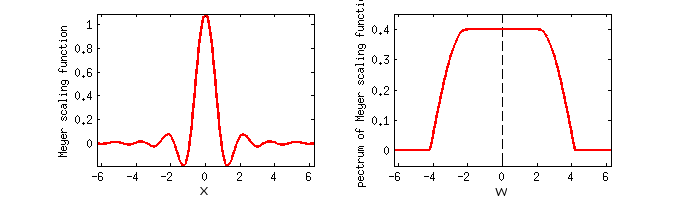
\includegraphics[height=4cm]{meyer.png}
    \caption{Meyer wavelet scaling function and its spectrum}
\end{center}\label{fig:Meyer}\end{figure}
\noindent 
$\phi_{j,k}(x)$ is localized in the frequency domain, and can be seen as a low pass filter.
Projecting a function $f \in L^2(\mathbb{R})$
onto $V_j$ gives a bandlimited approximation of $f$.
As $j$ increments by $1$, the bandwidth of the low pass filter will increase by a
factor of $2$,
so does the approximation resolution.
Besides, $\phi_{j,k}(x)$ is localized in $x$, i.e.
$\phi_{j,k}(x)\rightarrow 0$ as $x\rightarrow \pm \infty$.
Given $j$ and $k$,
$\left<f,\phi_{j,k}\right>$ effectively controls 
the shape of $P_{V_j} f$ only within a bounded domain centered at $\frac{k}{2^j}$.
This will be an important property when we discuss the concept of \emph{excited parameter domain}
in section \ref{adaptive}. In practice, it's infeasible and unnecessary to include all $\phi_{j,k}$
$k\in\mathbb{Z}$ into the basis library for a given $j$.
For example, in the 1D water-oil displacement process 
\cite{Buckley Leverett}, the water saturation $u$ satisfies $0\le u\le 1$. Therefore, it's 
unnecessary to consider $k$ for which $\frac{k}{2^j} \gg 1$ or $\frac{k}{2^j} \ll 0$.
We will discuss this topic in greater detail in section \ref{adaptive}.\\

\noindent In Eqn\eqref{first equation} and Eqn\eqref{first equation 2}, we notice that
adding a constant to $F$'s and $g$'s does not change the equations. In other words,
it suffices to approximate the flux functions' gradients instead of the flux function value.
Therefore, we consider the following functions:
\begin{equation}
    \bar{\phi}_{jk}(x) = \int_{-\infty}^x \phi_{j,k}(\tau)\;\textrm{d}\tau
\end{equation}
The gradient of $\bar{\phi}_{jk}(x)$ is local in frequency and
local in $x$. 
In this section, we will use $\left\{\bar{\phi}_{jk}\right\}$, $k\in \mathbb{Z}$ with
a fixed $j$ as the basis library for the flux function. \\

\noindent For flux functions $F(\tilde{u})$, $\tilde{u}\in \mathbb{R}^n$, $n>1$, the analogy of
basis functions is straightforward.
The MRA for $L^2(\mathbb{R}^n)$ is 
$V_{j_1}\otimes V_{j_2}\otimes \cdots \otimes V_{j_n}$, with
$\{j_1,j_2,\cdots,j_n\}\in \mathbb{Z}^n$ \cite{wavelet mallat, Dijkema book}.
Given $\mathbf{j} = \left\{j_1,\cdots,j_n\right\}$, The basis is
\begin{equation}
   \mathbf{\phi}_{\mathbf{j},\mathbf{k}} = \phi_{j_1,k_1}(x_1)\cdots \phi_{j_n,k_n}(x_n)\,,
   \quad \mathbf{k}\in\mathbb{Z}^n
\end{equation}
Therefore, the basis for the twin model flux function is
\begin{equation}
   \bar{\mathbf{\phi}}_{\mathbf{j},\mathbf{k}} = \bar{\phi}_{j_1,k_1}(x_1)
   \cdots \bar{\phi}_{j_n,k_n}(x_n)\,,
   \quad \mathbf{k}\in\mathbb{Z}^n
   \label{basis flux wavelet}
\end{equation}
Below we plot $\bar{\phi}_{0,0}(x)$ and $\bar{\phi}_{\mathbf{0},\mathbf{0}}(x_1,x_2)$ 
integrated from Meyer scaling function.
\begin{figure}[H]\begin{center}
    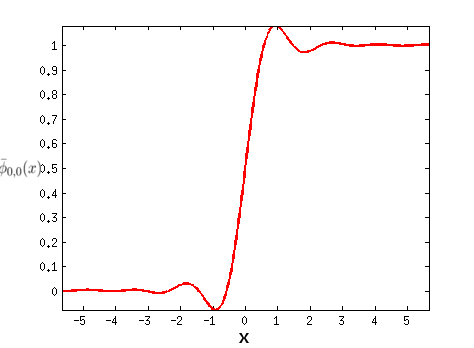
\includegraphics[height=5cm]{basis.png}
    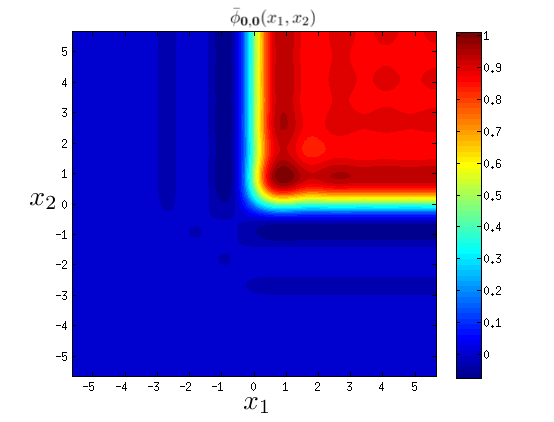
\includegraphics[height=5cm]{basis_2D.png}
\end{center}
\caption{$\bar{\phi}_{0,0}$ in 1D and 2D, integrated from Meyer wavelet scaling function}
\label{fig:Meyer Basis}
\end{figure}
%\noindent Clearly, using Eqn\eqref{basis flux wavelet} as the basis for the flux functions
%will be problematic for high dimensional $\mathbf{x}$. We will address this problem
%in section \ref{adaptive}.\\

\noindent Although function approximation with wavelet scaling function has mathematical
rigor, $\bar{\phi}$'s are not ideal bases for our problem. Firstly, the
integral of 1D scaling function is rippled, as can be seen in the Meyer wavelet example.
This is due to the \emph{localization in frequency}
property of scaling functions, known as the Gibbs phenomenon. 
The rippled flux may cause shock waves in hyperbolic equation simulations.
Indeed, the property of localization in frequency is not necessary in our
twin model problem.
Secondly, generally $\bar{\phi}$ does not have an analytical expression. 
So $\bar{\phi}$ must be evaluated by numerical integration or interpolation
using a lookup table, which can be more computationally intensive than
anlytical expressions. Therefore, we prefer a \emph{monotonic} and \emph{analytical}
 approximation for $\bar{\phi}$.\\

\noindent We choose a sigmoid function to replace $\bar{\phi}_{0,0}$:
\begin{equation}
    \bar{\phi}_{0,0}(x) = \frac{1}{2}\left(\tanh(\beta x)+1\right)\,,
\end{equation}
where $\beta$ is a constant determining the gradient of the function at $x=0$.
And
\begin{equation}
    \bar{\phi}_{j,k}(x) = \frac{1}{2} \left\{
        \tanh\left(\beta(2^j x-k)\right) +1
    \right\}
    \label{phijk}
\end{equation}
Or if we don't specify resolution on a dyadic grid $2^j$, we can write Eqn\eqref{phijk} as
\begin{equation}
    \bar{\phi}_{r,k}(x) = \frac{1}{2} \left\{
        \tanh\left(\beta(r x-k)\right) +1
    \right\}\,,
    \label{phirk}
\end{equation}
where $r>0$.
Without further specifications we'll choose $\beta=1.5$.
Below we plot $\bar{\phi}_{0,0}(x)$ and $\bar{\phi}_{\mathbf{0},\mathbf{0}}(x_1,x_2)$ 
using the sigmoid function.
\begin{figure}[H]\begin{center}
    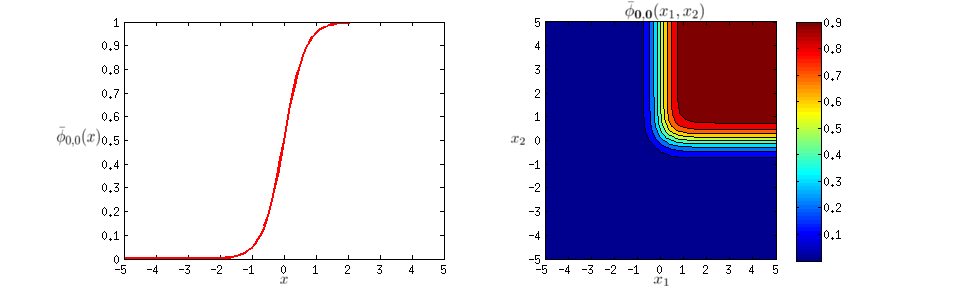
\includegraphics[height=5cm]{sigmoid_basis.png}
    \caption{$\tanh$ sigmoid function in 1D and 2D}
    \label{fig:sigmoid basis}
\end{center}\end{figure}


\subsection{Numerical example: twin model with fixed structure}
\label{fixed numerical example}
In this section we demonstrate a numerical example for fitting a twin model with fixed structure.
Consider a 1D Buckley-Leverett equation
\begin{equation}
    \frac{\partial u}{\partial t} + \frac{\partial F(u)}{\partial x} = 0\,\quad x\in[0,1]\,,\; t\in[0,1]
    \label{BL eqn}
\end{equation}
with periodic boundary condition
\begin{equation}
    u(x=0) = u(x=1)
\end{equation}
and initial condition
\begin{equation}
    u(t=0) = u_0
\end{equation}
Buckley-Leverett equation is a simple model for 1D, two-phase, porous media flow driven by
capillary pressure and Darcy's law \cite{Buckley Leverett}. $u$
indicates one phase's saturation and $0\le u\le 1$.
The flux function $F(u)$ depends on the phases and the porous media. 
A popular $F(u)$ is
\begin{equation}
    F(u) = \frac{u^2}{1+A(1-u)^2}\,,
    \label{BL flux}
\end{equation}
where $A$ is a constant. In the following we assume the blackbox simulation
solves Eqn\eqref{BL eqn} with the flux given by Eqn\eqref{BL flux}, and $A=2$.
\\

\noindent Assume $F(u)$ is unknown, we will fit a twin model 
using the blackbox simulation.
As discussed in section \ref{general formulation} and
\ref{basis selection}, the twin model can be written as
\begin{equation}
    \frac{\partial \tilde{u}}{\partial t} + \frac{\partial}{\partial x}\,
    \left(\sum_{k=1}^m \xi_k \bar{\phi}_{r,k}(\tilde{u})\right) = 0
    \label{twin model 3}
\end{equation}
with the same initial and boundary conditions. We will
use Eqn\eqref{phirk} for $\bar{\phi}$. Both the black-box simulation
and the twin model use a second order finite volume discretization and 
Crank-Nicolson time integration scheme.\\

\noindent We need to determine $r$ and the range for $k$ a prior. 
A larger $r$  means higher resolution of the flux, but the twin model will be
more computationally costly to fit. For this example,
we specify $r=10$. Besides, not all $k\in \mathbb{Z}$
are required in the twin model. As mentioned before, the gradient of
each basis indexed by $k$ is non-zero only around $[\frac{k}{r}-\frac{1}{\beta r},
\frac{k}{r}+\frac{1}{\beta r}]$. In our problem, $0\le u\le 1$, so it suffices
to choose corresponding $k$'s. We will choose $k=-1,0,\cdots, 11$.\\

\noindent The objective of fitting the twin model is given in Eqn\eqref{objective twin model},
and is itself an optimization.
We use an automatic differentiation module \textit{numpad} \cite{numpad} to compute
$\frac{dJ}{d\xi_k}\,, k=1,\cdots, m$.
Since the gradient information is available, we consider using a quasi-Newton method
for the optimization. Quasi-Newton methods build the Hessian approximation iteratively 
using gradient, and can greatly accelerate convergence \cite{Quasi-Newton Review}.
When the degree of freedom of the optimization is high, the memory required to 
store the Hessian matrix can be large. To reduce the memory requirement, 
we can use the \emph{low-memory Broyden-Fletcher-Goldfarb-Shannon} (L-BFGS) algorithm
\cite{nlopt, LBFGS, Eric master thesis}. 
L-BFGS approximates the Hessian using only the gradients at newer previous iterations,
and inverse the approximated Hessian efficiently using the Sherman-Morrison formula.
For this work, we
use the implementation of L-BFGS in Nlopt \cite{nlopt}.\\

\noindent Although the objective is to minimize 
$
\sum_{i=1}^{N}\sum_{k=1}^{T} \left(\tilde{u}_{ik} - u_{ik}\right)^2 \Delta t_k
\left| \Delta \mathbf{x}_i \right|
$, we will not use it as the objective function directly and perform optimization
in one shot. If $\tilde{F}(u)$ deviates from $F(u)$ a lot, then $\tilde{u}(x,t)$
can deviate from ${u}(x,t)$ significantly even at a small $t$. 
Therefore, solving the twin model and its adjoint in $t=[0,T]$ without
an educated $\tilde{F}(u)$ can be a waste of computation 
resources. To improve efficiency, we propose a progressive optimization
procedure:\\
\fbox{\parbox{\textwidth}{
\begin{algorithm}[H]
    $\xi^*=\mathbf{0}$\;
    Set integers $2= i_1< \cdots < i_M=T$\;
    \For{$I=i_1,\cdots, i_M$}{
        Optimize
        $$
           \xi^* \leftarrow \arg\min_{\xi} 
           \sum_{i=1}^{N}\sum_{k=1}^{I} \left(\tilde{u}_{ik} - u_{ik}\right)^2 \Delta t_k 
           \left| \Delta \mathbf{x}_i \right|
        $$
        with initial guess $\xi^*$.
  }
  \caption{Progressive optimization procedure}
  \label{progressive algo}
\end{algorithm}
}}\\

\noindent Notice $k=1$ corresponds to the initial condition. Since the twin model
uses the same initial condition as the black-box model, $\tilde{u}_{i1} - u_{i1}$
is always zero.
Choosing the integer sequence $i_1,\cdots,i_M$ can be problem dependent.
Our experience shows the sequence should be denser at small $i$, and sparser at larger $i$.
The tolerance of each sub-optimization problem does not need to be tight,
except for the last iteration where $I=T$.
In our problem, we use $i_l = \min\left\{ 1+2^l, T\right\}$,
a relative tolerance of $10\%$, and maximum $10$ iterations for the sub-optimization problems.\\

\noindent The initial condition is shown in Fig \ref{fig:initial condition}. Notice
$u_0$ does not cover the entire range of 
$0\le u\le 1$: we have $\max(u_0) =0.89$, $\min(u_0) = 0.07$.
\begin{figure}[H]\begin{center}
    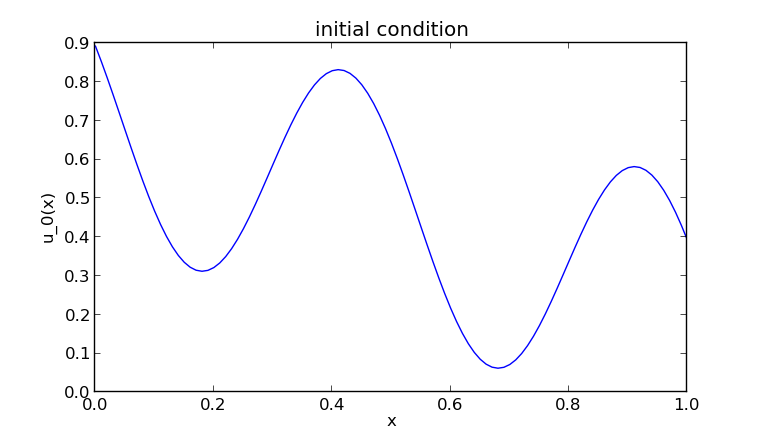
\includegraphics[height=4cm]{initial_condition.png}
    \caption{Initial condition $u_0(x)$}
    \label{fig:initial condition}
\end{center}\end{figure}
\noindent In Fig \ref{fig:flux compare} we compare the converged twin model's flux $\tilde{F}(u)$ and its gradient $\frac{d\tilde{F}}{du}$
with $F(u)$ and $\frac{dF}{du}$. The range
$u\in [\min(u(t,x)), \max(u(t,x))]$ is colored green.
\begin{figure}[H]\begin{center}
    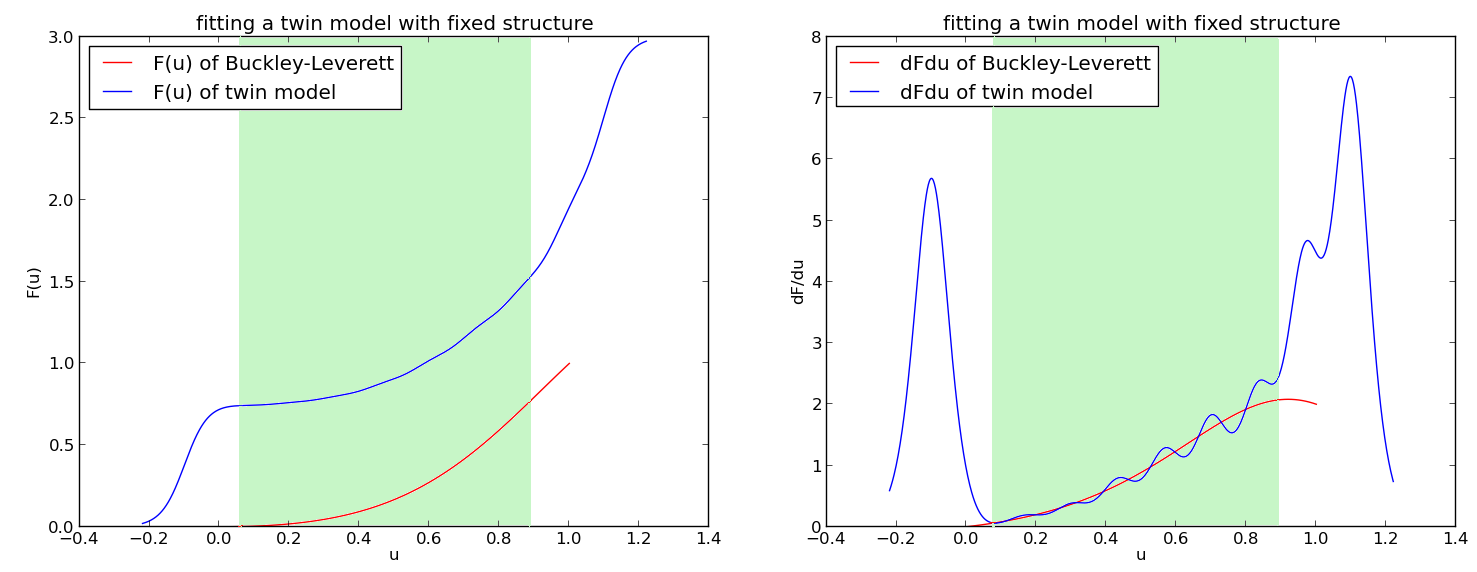
\includegraphics[height=5cm]{fit_flux_2.png}
    \caption{Compare $F(u)$ and $\frac{dF}{du}$ with $\tilde{F}(u)$ and $\frac{d\tilde{F}}{du}$}
    \label{fig:flux compare}
\end{center}\end{figure}
\noindent In Fig \ref{fig:sol compare} we compare the solution $u(t,x)$ with the converged
twin model's solution $\tilde{u}(t,x)$.
\begin{figure}[H]\begin{center}
    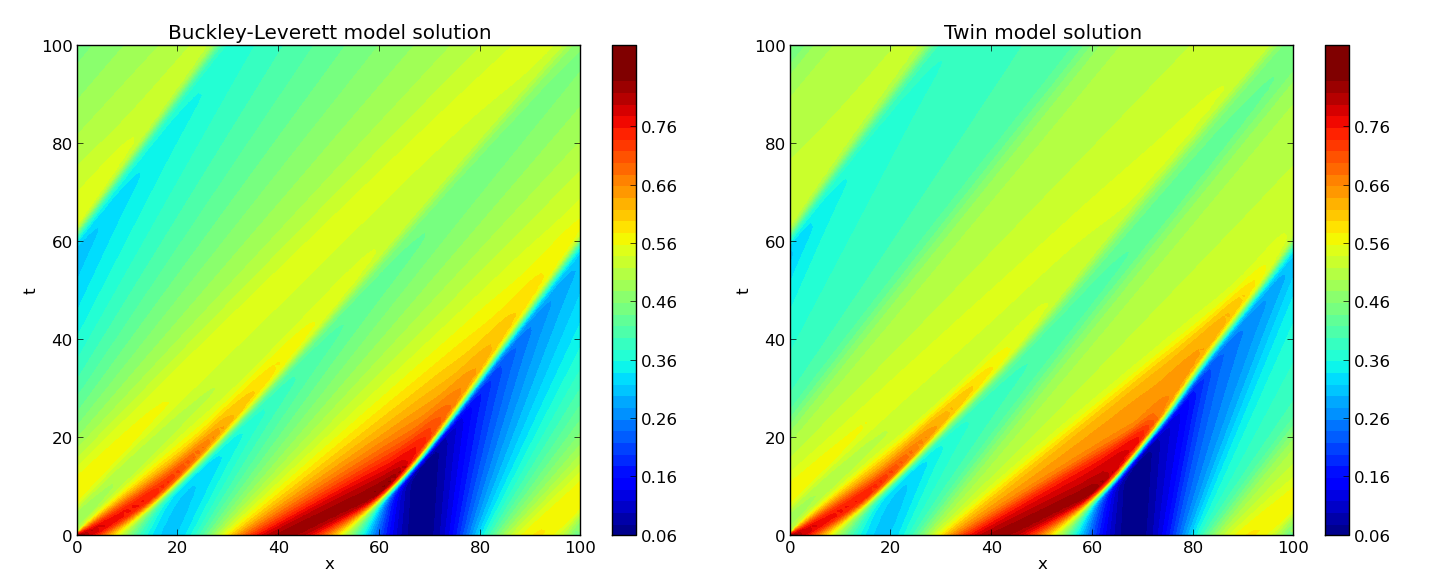
\includegraphics[height=5cm]{BL_sol.png}
    \caption{Compare $u(t,x)$ with $\tilde{u}(t,x)$}
    \label{fig:sol compare}
\end{center}\end{figure}

\noindent If we increase the flux resolution, the flux and the solution should have a better fit.
For example, we use $r=30$, $k=-3,\cdots,33$. The flux comparison is shown in Fig
\ref{fig:flux compare 30}
\begin{figure}[H]\begin{center}
    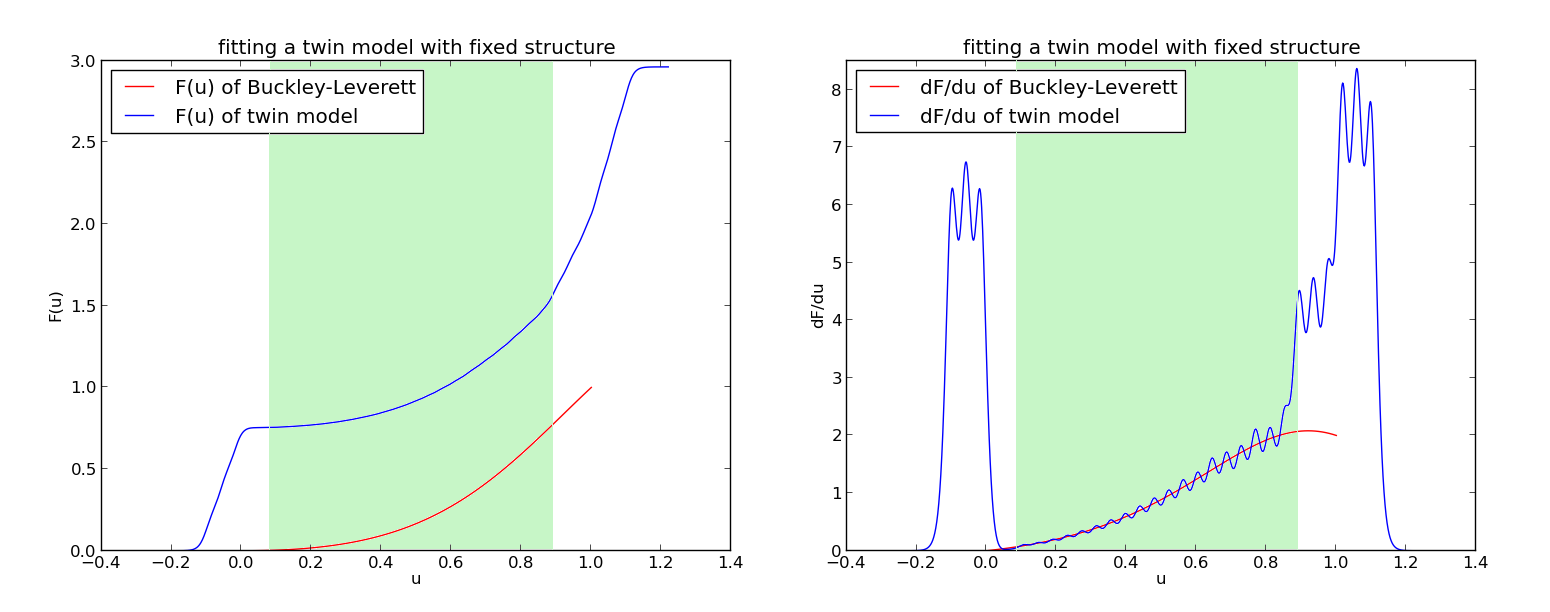
\includegraphics[height=5cm]{fit_flux_30_1.png}
    \caption{Compare $F(u)$ and $\frac{dF}{du}$ with $\tilde{F}(u)$ and $\frac{d\tilde{F}}{du}$
             with higher flux resolution}
    \label{fig:flux compare 30}
\end{center}\end{figure}
\noindent The solution comparison is shown in Fig \ref{fig:sol compare 30}
\begin{figure}[H]\begin{center}
    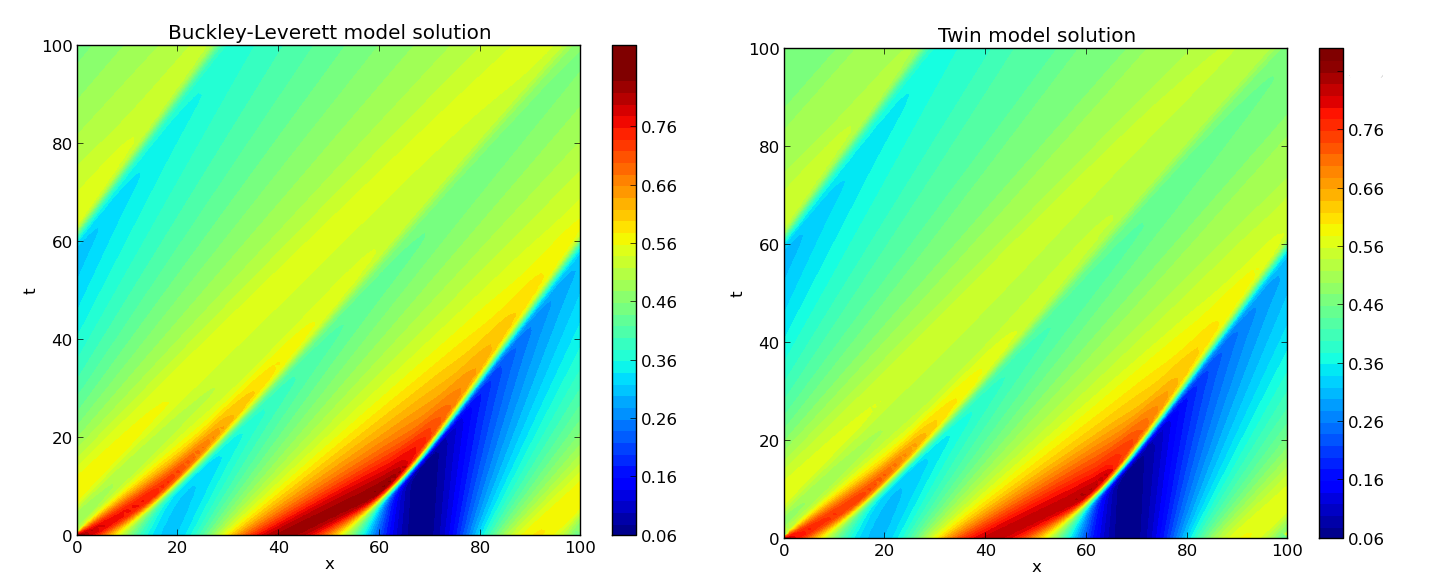
\includegraphics[height=5cm]{BL_sol_30.png}
    \caption{Compare $u(t,x)$ with $\tilde{u}(t,x)$ with higher flux resolution}
    \label{fig:sol compare 30}
\end{center}\end{figure}
\noindent Comparing Fig \ref{fig:flux compare}, \ref{fig:sol compare} 
with Fig \ref{fig:flux compare 30}, \ref{fig:sol compare 30}, we observe a refined flux basis 
gives a more accurate twin model.
However, we seek for an educated way to adaptively refine the
basis and to control the computation cost.
Therefore we will investigate \emph{twin model with adaptive structure}
in the next section.

\subsection{Twin model with adaptive structure}
\label{adaptive}
A twin model with adaptive structure should be able to adaptively
refine its basis $\bar{\phi}$ on-the-fly during fitting the basis coefficients $\xi$.
For example, in section \ref{fixed numerical example}'s numerical example,
the value of $u(t,x)$, $t\in[0,T],\,x\in[0,1]$ is bounded, i.e.
$0< u_{\min}\le u(t,x)\le u_{\max} < 1$; therefore as long as 
$\nabla\tilde{F}(u) = \nabla F(u)$ for $u\in[u_{min},u_{max}]$, we will have
$\tilde{u}(t,x) = u(t,x)$ for $t\in[0,T]$ and $x\in[0,1]$.
In other words, in the numerical example, $\nabla \tilde{F}(u) = \nabla F(u)$ for $u\in [0,1]$
is a sufficient but not necessary condition
for $\tilde{u}(t,x) = u(t,x)$. 
Intuitively, for some domains $u$, $\nabla \tilde{F}(u)$ has to approximate $\nabla F(u)$
accurately in order to give a good space-time solution match.
We will call such domains \emph{excited domain}, written as $\mathcal{E}$. 
Notice the excited domain is not a domain of space or time.  
Clearly $\mathcal{E}$ depends on $u(t,x)$.
For $u$ not inside $\mathcal{E}$,
$\nabla \tilde{F}(u)$ will have little or no effect on the solution match; therefore
we may not certify $\nabla \tilde{F}(u)$'s accuracy outside $\mathcal{E}$
no matter how closely the solutions match.
As mentioned in section \ref{basis selection}, we are interested in the problem of basis
selection. Basis selections should only be navigated to $\mathcal{E}$.\\

\noindent Consider a twin model solving
\begin{equation}
    \frac{\partial\tilde{u}(t,x)}{\partial t} + \nabla \cdot 
    \tilde{F}(\mathcal{D} \tilde{u}, \kappa) 
    = q(\tilde{u},c(t,x))\,, \quad \tilde{u}(t,x) \in \mathbb{R}^n\,,
    \label{twin equation def}
\end{equation}
We define the excited domain $\mathcal{E}$ by its complement $\bar{\mathcal{E}}$:\\
\fbox{\parbox{\textwidth}{
\begin{definition}
    Given a primal model, its discretized solution of $u(t,x)$, and
    a twin model Eqn\eqref{twin equation def},
    the excited domain $\mathcal{E}$ is a domain of $\tilde{F}(\cdot)$.
    Let the complement of $\mathcal{E}$ be $\bar{\mathcal{E}}$.
    Consider a perturbed twin model flux $\tilde{F}_{\delta}(\cdot) =F(\cdot)+ 
    \delta(\cdot)$.
    The perturbed twin model gives the discretized solution $\tilde{u}_{\delta}$.\\

    A set $e \subseteq \bar{\mathcal{E}}$ if and only if
    $$ \frac{1}{T}
    \sum_{i=1}^{N}\sum_{k=1}^{T} \left(\tilde{u}_{\delta, ik} - u_{ik}\right)^2 \Delta t_k
    \left| \Delta \mathbf{x}_i \right|$$
    is a constant for
    any $\delta$ with $\textrm{support}[ \delta] = e$.
\end{definition}
}}\\

\noindent This definition requires $F$ a prior, therefore it is not directly implementable.
The definition also requires enumeration of all possible $\delta$ to validate $\mathcal{E}$.
In practice, we can only validate a finite set of $\delta$, for example the basis function library
$\bar{\phi}$.
\\

\noindent Basis selection may be performed by regularization \cite{Lasso variable selection,
Critical review of variable selection}. 
For example, it has been shown that basis selection can be performed by having a
Lasso regularization term in the solution mismatch. In our problem, the metric of
solution mismatch with Lasso regularization would be
\begin{equation}
    \frac{1}{T}
    \sum_{i=1}^{N}\sum_{k=1}^{T} \left(\tilde{u}_{\epsilon\delta, ik} - u_{ik}\right)^2 \Delta t_k
    \left| \Delta \mathbf{x}_i \right|
    + \lambda \|\xi\|_1\,,
    \label{Lasso mismatch}
\end{equation}
where $\|\cdot\|_1$ is the $L_1$ norm. 
We will delay the discussion of Lasso regularization to later in this section. 
Clearly, a straightforward minimization of Eqn\eqref{Lasso mismatch} requires solving the twin model 
for $\tilde{u}$ in $[0,T]$.
As mentioned in section \ref{fixed numerical example}, unless $\tilde{u}(\tau)$
is reasonably close to $u(\tau)$, it does not make sense to keep solving the twin model for $t>\tau$.
Therefore, we should not let $\tilde{u}$ deviates from $u$ a lot.
We propose a basis selection scheme for time-dependent
twin model \emph{without solving the twin model in $[0,T]$}.\\


\noindent 
To restrict $\tilde{u}$ from large deviation from $u$, we propose a basis selection scheme
that does not require solving the twin model in $[0,T]$.
Define \emph{global error}:
\begin{equation}
    Err_{G} = 
    \frac{1}{T}\sum_{i=1}^{N}\sum_{k=1}^{T} \left(\tilde{u}_{ik} - u_{ik}\right)^2 \Delta t_k
    \left| \Delta \mathbf{x}_i \right|
    \label{global error}
\end{equation}
and \emph{local error}:
\begin{equation}
    Err_{L} = 
    \frac{1}{T}\sum_{i=1}^{N}\sum_{k=1}^{T} \left(\tilde{u}^\prime_{ik} - u_{ik}\right)^2 \Delta t_k
    \left| \Delta \mathbf{x}_i \right|
    \label{local error}
\end{equation}
Here $u$ is the \emph{one-shot} solution of the 
twin model solving from $t=0$ to $t=T$ with initial condition $u_0$.
$\tilde{u}^\prime_k$ is the solution of the twin model at $t=t_{k}$, solving from $t=t_{k-1}$
with initial condition $u_{k-1}$, for just one timestep. In other words, 
we solve $\tilde{u}^\prime$ with restart for every timestep, whose
initial condition is given by $u$ at a previous timestep.
We illustrate the idea in Fig \ref{fig:tmodelrestart}.
\begin{figure}[H]\begin{center}
    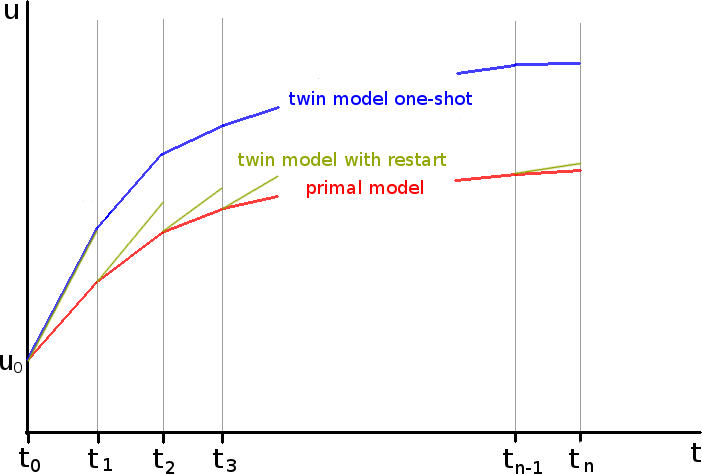
\includegraphics[height=5cm]{sketch2.png}
    \caption{illustration of twin model with restart.}
    \label{fig:tmodelrestart}
\end{center}
\end{figure}

\noindent If we are able to bound $Err_G$ with $Err_L$, we are guaranteed a good solution
match even if we do not solve for the one-shot solution $\tilde{u}$. Under what condition
can we bound $Err_G$? We give the following theorem.\\
\fbox{\parbox{\textwidth}{
\begin{theorem}
    \textbf{Global-local error}\\
    Consider the timestepwise mapping of the twin model
    \begin{equation}
        G:\, \mathbb{R}^n\mapsto\mathbb{R}^n,\, \tilde{u}^i\rightarrow 
        G\tilde{u}^i = \tilde{u}^{i+1}\,,\quad i=1,\cdots, n\,.
    \end{equation}
    If $G$ is a Lipschitz continuous mapping with constant $\alpha$
    \begin{equation}
        \|Gx-Gy\|_{L_2} \le \alpha \|x-y\|_{L_2}
    \end{equation}
    then 
    \begin{equation}
        Err_G \le (1+\alpha+\cdots+\alpha^{n-1}) Err_L\,.
    \end{equation}
    If $\alpha < 1$, then
    \begin{equation}
        Err_G < \frac{1}{1-\alpha}Err_L
    \end{equation}
    \label{theorem: 1}
\end{theorem}
}}\\

\noindent In practice, the assumption of $\alpha<1$ may not be
guaranteed. Therefore a small local error may not guarantee a small global error,
for example for chaotic dynamical systems.
Therefore, we only consider the local error as a tool to select basis, not a tool
to finalize the twin model. After selecting
the basis using the local error metric, 
we will still use the global error metric to fit the twin model, for example
using algorithm \ref{progressive algo}.\\

\noindent Using the local error metric, we are able to reduce the twin model
into solving a series of one-timestep problems with restart. But in each one-timestep
problem, the numerical implementation of $\nabla\cdot$ in Eqn\eqref{twin equation def}
is nonlinear. If we approximate $\nabla\cdot$ linearly, we will be able to 
use the wealth of knowledge of linear system basis selection. 
Let $\nabla\cdot$ be approximated by a
finite difference operator $D$. Besides,
a stable time integration scheme of twin model's solver is necessary 
for theorem \ref{theorem: 1} to hold. Here
we let $\frac{\partial}{\partial t}$ be approximated by Backward Euler. 
Then Eqn\eqref{twin equation def} becomes
\begin{equation}
    -\frac{1}{\Delta t_k}\left(\tilde{u}_{k} - \tilde{u}_{k-1}\right) +q(\tilde{u}_k,c(t_k))
    =
    \sum_{i=1}^m \xi_i D\left(\bar{\phi}_i(\mathcal{D}\tilde{u}_k, \kappa)\right)\,,
    \quad k=1,\cdots, T
    \label{linear eqn}
\end{equation}
For the $k$th timestep, let
\begin{equation}
    P_{ki} = D\left(\bar{\phi}_i(\mathcal{D}\tilde{u}_k, \kappa)\right) \in\mathbb{R}^N\,,
\end{equation}
where $N$ is the number of spatial gridblocks, and $i$ is the basis index. Also let
\begin{equation}
    Y_k = -\frac{1}{\Delta t_k}\left(\tilde{u}_{k} - \tilde{u}_{k-1}\right) +q(\tilde{u}_k,c(t_k))
\in\mathbb{R}^N\,.
\end{equation}
We rewrite Eqn\eqref{linear eqn} as
\begin{equation}
    Y = P\xi\,,
    \label{linear selection}
\end{equation}
where
\begin{equation}\begin{split}
    P = \begin{pmatrix}
        P_{11} & \cdots & P_{1m}\\
        \vdots &        & \vdots\\
        P_{T1} & \cdots & P_{Tm}
    \end{pmatrix}_{NT\times m}
\end{split}\,,    \quad
    Y = \begin{pmatrix}
        Y_1\\
        \vdots\\
        Y_T
    \end{pmatrix}_{NT}\,,\quad
    \xi = 
    \begin{pmatrix}
        \xi_1\\
        \vdots\\
        \xi_m
    \end{pmatrix}_{m}
\end{equation}
Unlike linear regression, the objective of Eqn\eqref{linear selection} is not 
to compute $\xi$, but to select a subset of variables of $\xi$. This is a 
\emph{linear} variable dimensional reduction problem.
Existing methods can be categorized into two 
classes \cite{NARMAXbook}: One class is to rank the importance of the variables and to select 
a subset of important variables directly from candidate variables
\cite{Lasso variable selection, Billing
feature selection}. Another class is to transform the original variables into a new 
reduced dimensional space \cite{review dimensional reduction}.
One of the most popular methods of the second calss is principal component analysis (PCA)
\cite{PCA review}. Although PCA can be efficiently computed by singular value decomposition,
it has a disadvantage. Because the principal components depend on \emph{all} original
variables, they can be difficult to interpret \cite{NARMAXbook}. In the twin model
analysis, we want
a basis selection scheme that reflects the excited domain $\mathcal{E}$. Therefore,
we will focus on the first class of methods.\\

\noindent Linear variable selection is a rich field. It considers a linear model
where each response variable $y_i$ relates with predictors $x_{ij}$ as follows
\begin{equation}
    y_i = \xi_0 + \sum_{j=1^m} x_{ij}\xi_j + \epsilon_i \,, \quad i=1,\cdots, N\,.
\end{equation}
$\epsilon$'s are independent noises. Some of the $m$ predictors may be unhelpful
for predicting $y$, and can be deleted. The task of variable selection is to decide
which subset of of variables should be deleted in order to get the \emph{best} equation
\cite{Critical review of variable selection}
\begin{equation}
    y_i = \xi_0 + \sum_{j\in \mathcal{S}\in{1,\cdots,m}} x_{ij} \xi_j + \epsilon_i\,,
    \quad i=1,\cdots, N\,.
    \label{selected variable model}
\end{equation}
Different metrics of defining `best' lead to different variables selection recipes.
We can by no means give a complete review of the methods here. Instead, we will only review two 
most popular classes of methods: \emph{test-based methods}, and 
\emph{regularization-based methods}.\\

\noindent Test-based methods implements a sequence of hypothesis tests to select variables.
They include forward, backward, and stepwise sequential testings
\cite{stepwise variable selection, Critical review of variable selection}.
Forward methods start with an empty set of selected variables, then
sequentially add the most significant unselected variables,
for example the
forward orthogonal least squares method for variable selection \cite{Billing feature selection}.
Backward methods start with a full set of selected variables, then
prunes non-significant predictors one at a time.
The stepwise methods alternate between adding and removing variables. 
However, there has been some critics to test-based methods
\cite{Critical review of variable selection}:
Firstly, these methods select variables sequentially using a greedy approach.
But the combinations of the best players at each step may not yield the best team.
Secondly, the greedy heuristics do not have a firm justification in statistical theory. 
The testing-based methods attempt to find the best model without first defining what
`best' means.\\

\noindent In contrast, regularization-based methods first define a metric of model goodness,
then search for the best model that maximize the metric. 
The metric is generally the \emph{penalized log likelihood}:
\begin{equation}
    \ell(\mathbf{x},\mathbf{y},\xi) - c(\xi)\,,
\end{equation}
where $\ell$ is the likelihood, $c$ is a measurement of model complexity.
Generally the penalty term is
\begin{equation}
    c(\xi) = \lambda \sum_{j=1}^m |\xi^q|^{1/q}\,,\quad \lambda>0,\, 0\le q\le 2
\end{equation}
It can be shown subset selection emerges as $q$ is close to $0$.
Ridge regression chooses $q=2$, and has no effect of variable selection.
Methods based on Akaike information criterion (AIC) \cite{AIC} and Bayesian information
criterion (BIC) \cite{BIC} chooses $q\rightarrow 0$, with different choices of $\lambda$.
But they yields a non-convex problem which is less attractive for computation.
Lasso chooses $q=1$, which is the smallest value of $q$
that yields a convex problem \cite{Lasso variable selection}. 
The properties of variable selection and
computation efficiency motivate us to use Lasso to select basis.\\

\noindent We implement Lasso variable selection using a python module \emph{sklearn} \cite{sklearn}.
The result is shown in Fig \ref{fig:basis_selection_1} and Fig \ref{fig:basis_selection_2}.
\begin{figure}[H]\begin{center}
    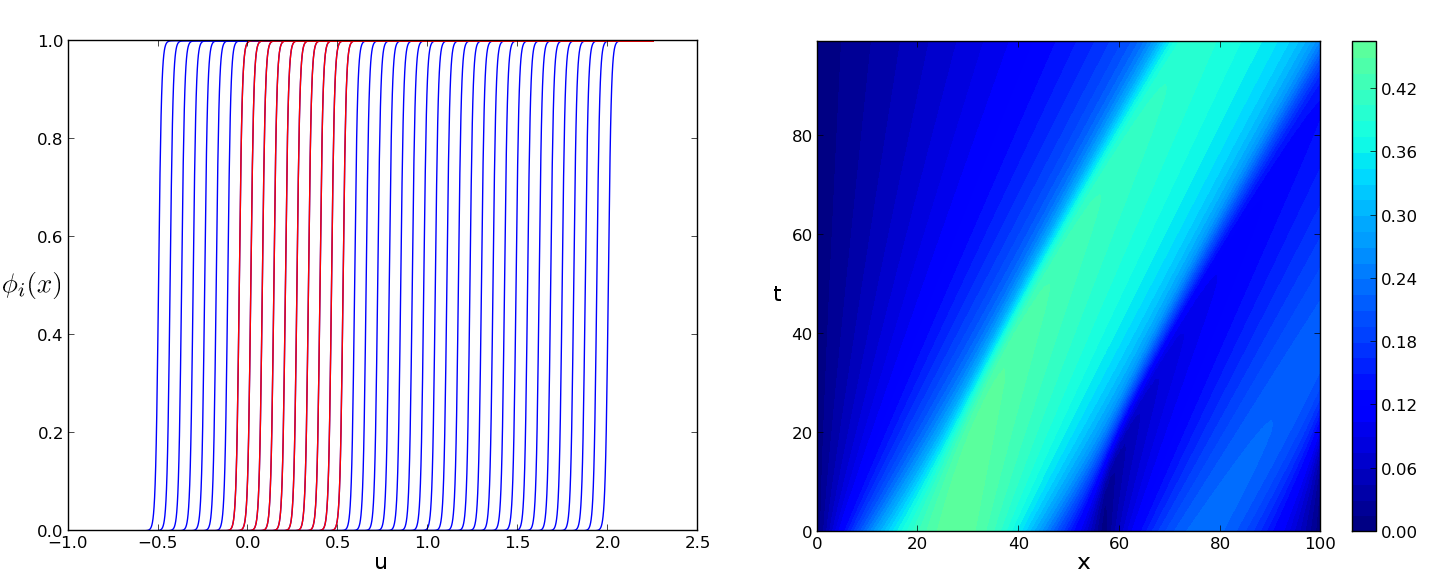
\includegraphics[height=5cm]{all.png}
    \caption{Basis selection using Lasso. The figure on the right side shows
    the primal model's solution $u(t,x)$. The figure on the left side shows all
    candidate bases. The selected bases are colored red. Notice how the selected
    bases correspond to the colorbar of the primal model solution.}
    \label{fig:basis_selection_1}
    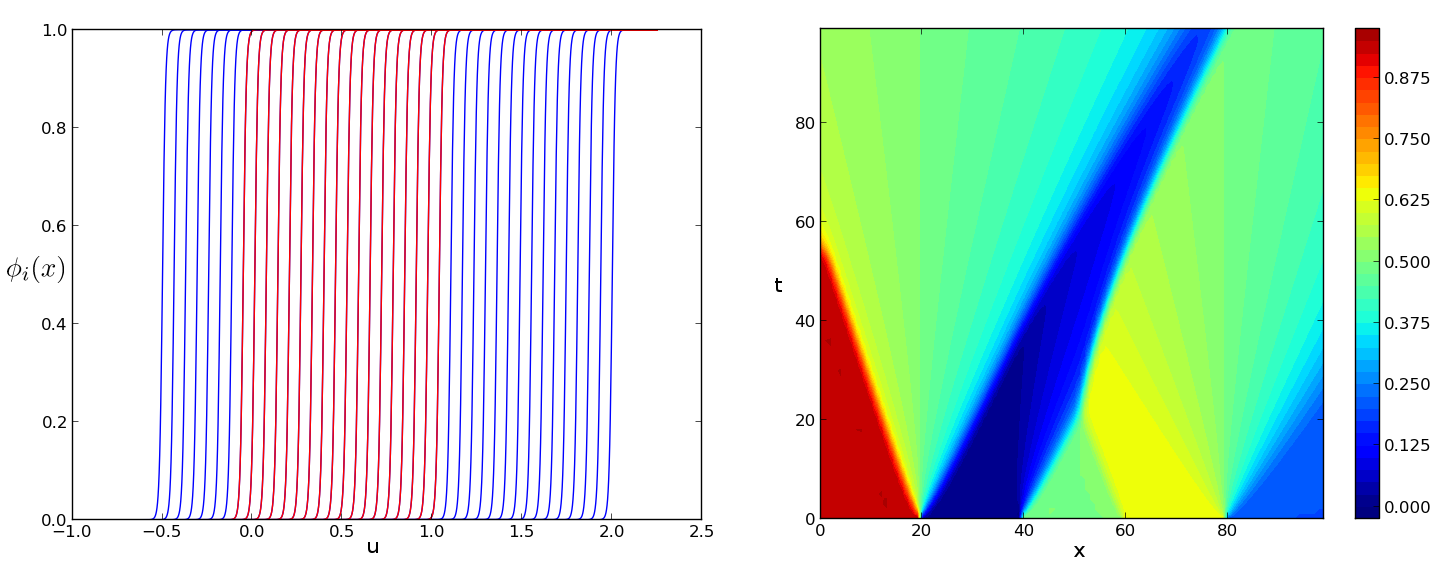
\includegraphics[height=5cm]{all2.png}
    \caption{Basis selection with a different $u(t,x)$. Notice
    how selected bases depend on the primal model solution.}
    \label{fig:basis_selection_2}
\end{center}
\end{figure}

\subsection{Future work}
\label{future work}
The sections above provide a framework to infer the twin model for time-dependent primal models 
with unknown flux functions. The framework can be extended to unknown source terms
straightforwardly. However, there are two issues to investigate.\\

\noindent Firstly, we need to extend the basis selection scheme to
time-independent twin model.
Right now, the basis selection scheme in section \ref{adaptive} is only for time-dependent PDEs.
Using a global-local error approach and a finite difference approximation, the basis
selection problem was reduced to a linear basis selection problem.
However, this approach is not suitable for time-independent twin model.
A candidate approach is to use Lasso regularization instead of Tikhonov regularization
in the metric of solution mismatch.
Unlike time-dependent twin model,
we may have to solve time-independent twin model to select basis.\\

\noindent Secondly, we need to explore the weighting scheme used in Eqn\eqref{minimizer twin model}.
Loosely speaking, choosing $w=1$ is equivalent to setting a uniform sample weight, where each `sample'
corresponds to the solution at a spatial and time grid point.
By using a variable $w$, we should be able to fine tune the twin model accuracy at different locations
in the excited domain $\mathcal{E}$. For example, should we assign a larger $w$
for regions with sparser samples? Or should we assign a larger $w$ for regions where
more interesting physics happen (e.g. around a shock wave)?
The weighting scheme may be ad hoc, but can possibly 
improve the twin model's accuracy for specific numerical examples.\\


%\noindent Thirdly, in section \ref{adaptive}, we discussed twin model with adaptive structure.
%The proposed approach constructs a \emph{fixed} candidate basis library 
%(Volterra series, wavelet scaling functions, and sigmoid functions), then selects a subset of basis
%from the library.
%However, the cardinality of the basis library can be high for flux functions with a large number
%of inputs, for example $F(u_1,\cdots,u_n)$ with a large $n$. Besides, the proposed basis
%library may be inefficient to represent flux of the form $F(\mathbf{w}^T \mathbf{u})$, where 
%$\mathbf{w}$ is
%a constant vector. Although $F(\mathbf{w}^T \mathbf{u})$ can be reduced to a univariate
%function by a change of variable $u^* = \mathbf{w}^T \mathbf{u} \in\mathbb{R}$, 
%the fixed basis library 
%can not take advantage of it.
%Therefore, the twin model method may be improved by choosing 
%a set of basis from an \emph{non-fixed} basis library.
%A literature survey is required 
%to determine the most appropriate method to use.

\newpage
\section{Optimization with twin model}
\noindent In chapter \ref{gradient_surrogate},
we developed twin model as a physics-based surrogate method.
How should we leverage this surrogate to facilitate optimizations based on gray-box simulations?
In this chapter, we answer this question by developing a provably convergent optimization scheme.
We also demonstrate our method's superiority for optimization with high-dimensional controls.\\

\subsection{Motivation of the Bayesian approach}
We are interested in optimization problems of the following form
\begin{equation}\begin{split}
    \min_{c\in\mathcal{C}} & J(u,c)\\
    \textrm{where}\; u\; \textrm{satisfies}& \;\; \mathcal{R}(u,c) = 0\\
    \textrm{subject to} \; \mathcal{C} & = \left\{\left. c\in\mathbb{R}^d\right| 
    A c\le b, V(c)\le 0\right\}
\end{split}\label{general opt}
\end{equation}
where $u(t,\mathbf{x})\in\mathbb{R}\,, t\in[0,T], \,x\in\Omega$
is the space-time solution of a PDE abstracted as
$\mathcal{R}$, with given initial and boundary conditions.
The controls are $c\in\mathbb{R}^d$. 
There are $l$ linear constraints defined by $A\in\mathbb{R}^{l\times d}$ and $b\in\mathbb{R}^{l}$
and $s$ nonlinear constraints defined by $V(c)\in \mathbb{R}^s$. 
These linear and nonlinear constraints define a feasible region 
$\mathcal{C}\subseteq \mathbb{R}^d$. The evaluation of $J$ for a given $c$ requires
solving the PDE $\mathcal{R}(u,c)=0$ which can be computational costly, such
as large eddy simulation (LES) \cite{LES, LES oldest} 
and direct numerical simulation (DNS) \cite{DNS} in  
aerodynamic design problems. It is not uncommon for these simulations
to take days, weeks, or even longer on a cluster.
In addition to expensive evaluations of $J$, the evaluations of
nonlinear constraints $V(c)$ can be similarly expensive. For example, 
in airfoil design we may aim at reducing drag while keeping lift 
above a threshold value \cite{constraint lift}. Evaluating the lift of a given design
requires simulating the flow. Besides, we consider the PDE and its solver 
as a gray-box. Finally, we consider controls of high dimension, i.e. $d\gg 1$.\\

\noindent We start with optimization problem Eqn\eqref{general opt} with feasible region
$\mathcal{C}=\mathbb{R}^d$ for simplicity.
There are already many methods that deal with such optimizations. 
But as mentioned in section \ref{gradfree_gradbased}, these methods are not suitable
for our problem because they either require adjoint-based gradient of the PDE solver, 
or suffer from the curse of dimensionality. Can we utilize the twin model together
with the primal model, and develop an optimization scheme that addresses these challenges?\\

\noindent The question fits naturally into a \emph{multifidelity optimization (MFO)} framework.
MFO performs optimization with multiple models ranging from
low-fidelity to high-fidelity. Conventionally, low-fidelity models are cheaper to solve, but yield
results with less credibility; high-fidelity models are more credible, but more expensive
to solve. MFO balances computation investments between high- and low-fidelity models
in order to reach optimum with overall less computation cost.
In our problem, the primal model can be considered as a high-fidelity model, and the twin model
can be considered as a low-fidelity model.\\

\noindent MFO methods can take various flavors.
For example, an MFO method can be as simple as a two-stage optimization \cite{MFO: two stage}. 
In the first stage it optimizes with the low-fidelity model only. In the second stage
it optimizes with the high-fidelity model only, using the first stage optimum as the initial guess.
However, we are only interested in \emph{provably convergent} MFO methods.
Based on our literature review, there are three types of such methods:
\emph{pattern search MFO}, \emph{trust region MFO}, and \emph{Bayesian MFO}.
Each type can be viewed as 
extensions to their \emph{single-fidelity} versions respectively,
i.e. \emph{pattern search methods}, \emph{trust region methods}, and \emph{Bayesian 
optimization methods}. In the following let's review these methods and 
their corresponding MFO methods.\\

\noindent In \emph{pattern search methods}, the objective function $J$ is evaluated at a set of
trial points, called `mesh', adjacent to the current best $c$ in the design space. This
step is called a `poll step'.
If improvement in $J$ is obtained, the current best $c$ is updated; otherwise, the mesh size
is shrinked. 
These steps are iterated until convergence \cite{Pattern Search Convergence}.
Pattern search methods can takes advantage of low-fidelity models to reduce computation cost,
hereby \emph{pattern search MFO}.
It searches for improved design 
points using low-fidelity models before deciding whether to perform a poll step on
the high-fidelity model \cite{Pattern Search Convergence MFO}.
However, each poll step requires order $d$ high-fidelity model evaluations, which can
be too expensive to afford in our problem settings.\\

\noindent In \emph{trust region methods}, a functional surrogate is firstly constructed from
evaluations of $J$, then the surrogate is minimized within a trust-region to generate
a candidate design point. Depending on the availability of $\frac{\partial J}{\partial c}$,
the functional surrogate can either use the gradient information \cite{inexactgradient1},
or not use the gradient information \cite{jones1998, trustregionconn, trustregionwild}.
When a low-fidelity model exists,
the functional surrogate of $J$ can be replaced by the low-fidelity model, hereby
\emph{trust region MFO} \cite{simplified physics, coarse discretization}.
To improve MFO performance and guarantee convergence,
researchers have proposed using functional surrogates to account for 
the discrepancy $\Delta J = J_{high} - J_{low}$
between high- and low- fidelity models within the trust region
\cite{andrewras, andrew thesis}. However, there are two problems with trust region MFO.
Firstly, the convergence proof of such methods requires
a condition called \emph{fully-linearity} \cite{trustregionconn}. The fully-linearity
condition bounds the deviation of $\frac{dJ}{dc}$ between the high- and low-
fidelity models within the trust region. As mentioned in
chapter \ref{intro}, it can be hard to obtain the gradient from the primal model.
Therefore, it can be hard to certify fully-linearity and to support 
the convergence proof.
Secondly, at every iteration, only the model evaluations within or adjacent
to a trust region is actually used \cite{andrew thesis}. In our problem settings,
each high-fidelity model evaluation can be so expensive that we should use \emph{all}
high-fidelity evaluations available.
Therefore, trust region MFO is not suitable for our problem settings too.\\

\noindent In \emph{Bayesian optimization methods}, $J$ as a function of $c$
is assumed to be an unknown realization of a \emph{Gaussian process}. 
Bayesian optimization starts from a prior distribution of $J$, and
updates its posterior as new samples of $J(c)$ arrive. This procedure is also known as
\emph{Kriging} \cite{Krigingold, kriging}.
Then it constructs an \emph{acquisition function} $\rho: \mathcal{C}\mapsto \mathbb{R}\;
,\; c\rightarrow \rho(c)$ from the posterior, which measures
the expected utility of investing the next sample at $c$.
Finally, we choose the next sample as the maximizer of the acquisition function.
Bayesian optimization iterates over the posterior-update step and the 
$\rho$-maximization step until convergence \cite{Mockus Bayesian opt, practicalBayesianopt}.
There are two advantages of Bayesian optimization:
Firstly, Bayesian optimization uses all available model evaluations
to construct the posterior. Secondly, it balances \emph{exploration}
with \emph{exploitation} elegantly.
Given a set of samples $J(c)$, should we choose the next sample 
in a sparsely sampled region (exploration),
or in a region adjacent to the current best sample (exploitation).
Bayesian optimization makes a trade-off between exploration and exploitation 
via appropriate acquisition functions. This method is provably convergent
to the global optimal under mild requirement of the objective function 
\cite{Bayopt converge 2, convergenceBayesian}.
\\

\noindent When a low-fidelity model exists, Bayesian optimization methods
can be extended to \emph{Bayesian MFO}.
Let the high-fidelity model's objective function
be $J(c)$, and the low-fidelity model's objective function be $\tilde{J}(c)$.
Bayesian MFO assumes both $J(c)$ and $\tilde{J}(c)$ are unknown realizations
of (possibly different) Gaussian processes.
Loosely speaking, by connecting the high- and low-fidelity models using 
a Bayesian framework, we can better predict the high-fidelity model using
low-fidelity model evaluations.
Bayesian MFO assumes a \emph{Markov property}
between $J(c)$ and $\tilde{J}(c)$ \cite{KennedyOhagan2}:
\begin{equation}
    p\left[ J(c_0)\Big| \tilde{J}(c_0), \tilde{J}(c_1),\cdots, \tilde{J}(c_N)\right]
    = p\left[ J(c_0)\Big| \tilde{J}(c_0)\right]
    \,,\quad
    N\in \mathbb{Z}^+\,,
    \label{ohagan_assumption}
\end{equation}
where $p(\cdot|\cdot)$ indicates the posterior. In other words,
if we want to predict $J$ at $c_0$ using $\tilde{J}$, then it suffices to 
evaluate $\tilde{J}$ only at $c_0$; we will gain no further information on $J(c_0)$ 
by observing $J$ at $c\neq c_0$. This assumption is intuitive, and proves to be
very useful and convenient \cite{KennedyOhagan1, KennedyOhagan2}. 
By furthur assuming the Gaussian processes to be stationary, we can obtain
\begin{equation}
    \tilde{J}(c) = \rho J(c) + \epsilon(c)\,,
\end{equation}
where $\rho$ is a constant and $\epsilon(\cdot)$ is a realization of a Gaussian 
process. Assume we have evaluated $J$ at $\mathbf{c}=\{c_1,\cdots, c_{N_1}\}$,
and $\tilde{J}$ at $\mathbf{\tilde{c}} = \{\tilde{c}_1,\cdots, \tilde{c}_{N_2}\}$,
then the posterior of $J(c)$ can be constructed from the joint distribution
\begin{equation}
    p\left(J(c), J(\mathbf{c}), \tilde{J}(\mathbf{\tilde{c}})\right) 
    = \mathcal{N}\left(
    \begin{pmatrix}
        m\\ \mathbf{m} \\ \mathbf{\tilde{m}}
    \end{pmatrix},\,
    \begin{pmatrix}
        \textrm{var}(J(c)) &
        \textrm{cov}(J(c), J(\mathbf{c}) ) &
        \textrm{cov}(J(c), \tilde{J}(\mathbf{\tilde{c}}))\\
        \textrm{cov}(J(\mathbf{c}), J(c) ) & 
        \textrm{var}(J(\mathbf{c})) & 
        \textrm{cov}(J(\mathbf{c}), \tilde{J}(\mathbf{\tilde{c}}))\\
        \textrm{cov}(\tilde{J}(\mathbf{\tilde{c}}), J(c)) & 
        \textrm{cov}( J(\mathbf{c}), \tilde{J}(\mathbf{\tilde{c}}) ) & 
        \textrm{var}(\tilde{J}(\mathbf{\tilde{c}}))
    \end{pmatrix}
    \right)\,
    \label{joint distribution}
\end{equation}
where $m$ is the mean of $J$, $\tilde{m}$ is the mean of $\tilde{J}$, $\mathbf{m} =
m \mathbf{1}_{N_1}$, and $\mathbf{\tilde{m}} =\tilde{m}\mathbf{1}_{N_2}$.
The variance-covariances, known as \emph{kernels}, have to be selected \emph{a} prior.
However, these kernels are adaptive in that they have tunable parameters known as
\emph{hyperparameters}, so realizations of the Gaussian processes
can represent a wide class of functions \cite{RKHS aronszajn}. 
The estimation of the hyperparameters and $\rho, m, \tilde{m}$ will be discussed below.
The choice of kernels can be various, among the most popular ones are
squared exponential kernel and Matern kernel \cite{practicalBayesianopt}.
Because of the additional information of $\tilde{J}(\tilde{\mathbf{c}})$, 
we can estimate
$J(c)$ with less variance than using $J(\mathbf{c})$ alone.
This procedure is also known as \emph{coKriging} \cite{cokriging}. 
With the posterior obtained by the coKriging, Bayesian MFO maximizes the acquisition
function to select the next design point $c$ to evaluate $J$.\\

\noindent How should we apply our twin model to a Bayesian MFO framework?
Naturally we would think of a coKriging approach using Eqn\eqref{joint distribution}:
We would first simulate the primal model as a high-fidelity model
at an initial guess $c_0$. 
This gives us the space-time solution $u_0$ and the objective function $J(c_0)$.
We can train the twin model with $u_0$ using methods proposed in chapter 
\ref{gradient_surrogate}. The trained twin model, as a low-fidelity model, 
can be simulated to obtain $\tilde{J}$ at a set of new design points.
Finally, the posterior of $J(c)$ can be constructed using the joint distribution
Eqn\eqref{joint distribution}. We may repeat these steps while re-training 
the twin model at updated design points.\\

\noindent However, this approach is not suitable for our problem settings.
The twin model may not be very cheap to evaluate. Contrary to the conventional
ideology: ``low-fidelity model is cheap'', the twin model can 
be expensive to simulate. Twin model is itself a PDE simulator.
Unlike many commericial or open-source gray-box PDE simulators whose code is highly optimized
for efficiency,
the twin model code can be less efficient and more costly to solve. When
the design space dimension $d$ is high, explorations of the design space
using evaluations of $\tilde{J}$ suffers from the curse of dimensionality too.\\

\noindent To unleash the power of twin model, we propose using the twin model's gradient
$\frac{d\tilde{J}}{d c}$ instead of $\tilde{J}(c)$ for coKriging.
The twin model is an open-box and has the adjoint capability to compute $\frac{d\tilde{J}}{dc}$.
It has been shown that using the adjoint-based gradient information can 
reduce the number of function evaluations for Bayesian optimization
\cite{adjoint gradient cokriging without MLE, gradient kriging surrogate},
especially when $d$ is large. 
In our problem settings, we do not have access to the adjoint-based gradient $\frac{dJ}{dc}$,
but it is possible to approximate $\frac{dJ}{dc}$ by $\frac{d\tilde{J}}{dc}$.
We can't make general arguments about the approximation accuracy. 
Even if the twin model can reproduce the space-time solution of the primal model
at a training design point, we can't ascertain that their adjoints 
are close, for example when the twin model solves a chaotic system.
However, the theoretical flaw should not prohibit us from investigating
practical applications of twin model. Besides, later we will show that our optimization scheme 
converges to the global optimal for the primal model,
no matter how accurate or inaccurate the gradient approximation is.\\

\noindent Here is an example demonstrating why it can be promising to approximate
$\frac{\partial J}{\partial u}$ with $\frac{\partial \tilde{J}}{\partial u}$.
Consider the numerical example in section \ref{fixed numerical example}, where the
primal model solves:
\begin{equation}
    \frac{\partial \tilde{u}}{\partial t} + \frac{\partial}{\partial x}\,
    \left(F(u)\right) = c\,,
\end{equation}
for $c=0$, with $F(u)$ given by Eqn\eqref{BL flux}. We trained a twin model
Eqn\eqref{twin model 3} using the space time solution. We are interest in
the approximation quality of the twin model's gradient at $c$ adjacent to $c=0$.
The result is shown in 
\begin{figure}[H]\begin{center}
    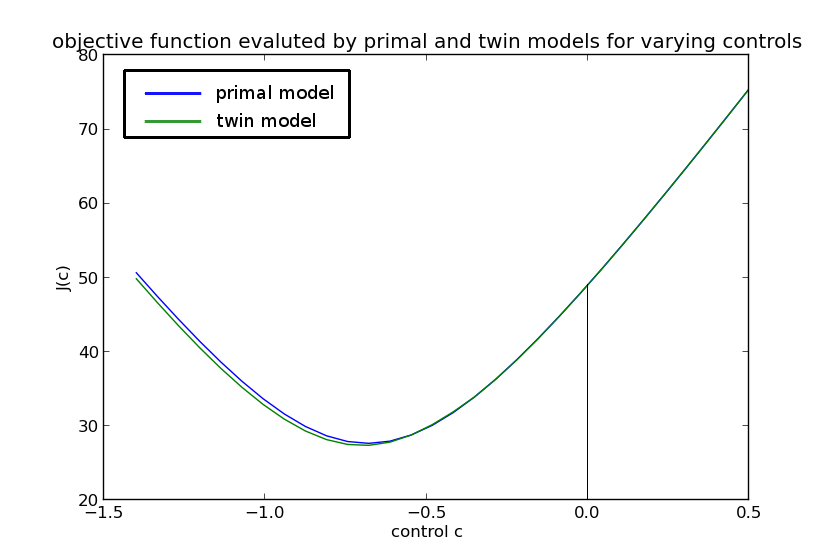
\includegraphics[height=6cm]{J_twin_vs_primal.png}
    \caption{Train the twin model at $c=0$, the resultant twin model gives good approximation for
    the $\frac{dJ}{dc}$.}
\end{center}\end{figure}
\noindent The result is encouraging as the gradient computed by the twin model gives a good approximation
of the gradient of the primal model. We reiterate that the good approximation quality benefits from 
the matching of space-time solution.



\subsection{Bayesian modeling of the primal and twin models}
\label{bayesian_model}
\noindent We model the relation of $\nabla J(c)$ and $\nabla \tilde{J}(c)$ as
\begin{equation}
    \nabla \tilde{J}(c) = \nabla J(c) + \epsilon(c)\,,
    \label{base Bayes model}
\end{equation}
Assume $\nabla J(c)$, $\nabla \tilde{J}(c)$, and $\epsilon(c)$ 
are realizations of stationary Gaussian processes. We first model the priors
of $\nabla J(c)$, $\nabla \tilde{J}(c)$, and $\epsilon(c)$, when no evalutions
of the high- and low-fidelity models are made.\\

\noindent For any $c_1$ and $c_2$, assume
$\epsilon(x)$ is an unknown realization of Gaussian process
$\mathcal{N}(\textbf{0}, K_{\epsilon}(\cdot,\cdot))$. 
$K_\epsilon: \mathbb{R}^n \times\mathbb{R}^n\mapsto \mathbb{R}$
\begin{equation}
    \quad K_{\epsilon}(c_1, c_2) =\boldsymbol{I}_{n\times n} 
    k_\epsilon(c_1, c_2; \theta_\epsilon)\,,
\end{equation}
where $\theta_\epsilon$ are the hyperparameters of the kernel.\\
$J(c)$ is treated as a realization of the Gaussian process 
$\mathcal{N}(\mu, K(\cdot,\cdot))$, 
$K: \mathbb{R}^n \times\mathbb{R}^n\mapsto \mathbb{R}$
where
\begin{equation}
    K(c_1, c_2) = k(c_1, c_2; \theta)\,.
\end{equation}
$\theta$ are the hyperparameters of the kernel.
Assume
\begin{equation}\begin{split}
    cov(\nabla J(c_1), \epsilon(c_2)) &= 0\\
    cov(J(c_1), \epsilon(c_2)) &= 0\,,
\end{split}\end{equation}
for any $c_1$, $c_2$.
Then
\begin{equation}
    \quad cov(J(c_1), \nabla \tilde{J}(c_2)) = cov(J(c_1), \nabla J(c_2))
\end{equation}
for any $c_1$, $c_2$.
There are multiple popular choices for the kernels.
Generally the squared exponential kernel is a default choice. However,
sample functions from this kernel are unrealistically smooth and may not
represent the objective function well. Another popular choice is the Matern kernel, especially 
$5/2$ kernel:
\begin{equation}
    K_0(c_1, c_2; \theta) \equiv \sigma^2 \left(1+\frac{\sqrt{5}d}{\rho}
    + \frac{5d^2}{3\rho^2}\right) \exp\left(-\frac{\sqrt{5}d}{\rho}\right)\,,
    \label{funkernel}
\end{equation}
where $d = \|c_1-c_2\|_{L_2}$. $\theta$ are the hyperparameters $\rho$ and $\sigma$.
The corresponding sample functions are twice differentiable, but not as
smooth as the square exponential kernel. It has been shown the Matern $5/2$ kernel 
outperforms other kernels in several Bayesian optimization problems \cite{practicalBayesianopt}.
Thus we choose the Matern $5/2$ kernel as our choice.
It is worth noting that the kernel function was chosen to be isotropic. 
In our problem, all the design parameters are the boundary points that controls 
the return bend geometry, so it makes sense to use a isotropic kernel for simplicity.
In general, the metric $d$ does not need to be isotropic, but this comes at the price
of having more hyperparameters.
\noindent Based on the assumptions above, we have
\begin{equation}
    K_1(c_1, c_2; \theta) \equiv
    \frac{\partial}{\partial c_2} cov(J(c_1), J(c_2)) =
    \sigma^2 \exp\left\{-\frac{\sqrt{5}d}{\rho}\right\}
    \left(\frac{5}{3\rho^2}
    + \frac{5\sqrt{5}d}{3\rho^3}\right) (c_1-c_2)
\end{equation}
and
\begin{equation}
    K_2(c_1, c_2; \theta) \equiv
    \frac{\partial^2}{\partial c_1\partial c_2} cov(J(c_1),J(c_2))
    = \sigma^2 \exp\left\{-\frac{\sqrt{5}d}{\rho}\right\}
    \left\{
        \left(\frac{5}{3\rho^2} + \frac{5\sqrt{5}d}{3\rho^3}\right)\boldsymbol{I}
        - \frac{25}{3\rho^4} (c_1-c_2) (c_1-c_2)^T
    \right\}
\end{equation}
We will model $J(c)$ as sampled function with the kernel Eqn\eqref{funkernel} with
hyperparameters $\theta = (\rho, \sigma)$.
We will model $\epsilon(c)$ as sampled function with the kernel
\begin{equation}
    \boldsymbol{I}_{n\times n} K_0(c_1, c_2; \theta_\epsilon)
    \label{noise kernel}
\end{equation}
with hyperparameters $\theta_\epsilon = (\rho_\epsilon, \sigma_\epsilon)$.
Suppose we sample $J$ on $\mathbf{c}$, and sample $\nabla \tilde{J}$ on
$\mathbf{\tilde{c}}$, then the joint probability of $J(c)$ at an unsampled $c$ 
and the sampled data can be constructed.
Specifically, the joint probability is a Guassian process with mean
\begin{equation}
    \left(\mu , \boldsymbol{\mu} , \mathbf{0}\right)^T
\end{equation}
and covariance
\begin{equation}
    \begin{pmatrix}
        K_0 (c, c; \theta) & K_0(c, \mathbf{c};\theta) & K_1(c, \tilde{\mathbf{c}}; \theta)\\
        K_0 (c, \mathbf{c}; \theta)^T & K_0(\mathbf{c}, \mathbf{c};\theta) 
        & K_1(\mathbf{c}, \tilde{\mathbf{c}}; \theta)\\
        K_1(c, \tilde{\mathbf{c}}; \theta)^T & K_1(\mathbf{c},\tilde{\mathbf{c}}; \theta)^T &
        K_2(\tilde{\mathbf{c}}, \tilde{\mathbf{c}}; \theta) + 
        K_\epsilon (\tilde{\mathbf{c}}, \tilde{\mathbf{c}}; \theta_\epsilon)
    \end{pmatrix}
\end{equation}
In practice, because the high-fidelity model
is never simulated for infinite time to compute the time average,
the sampling of $J$ can be noisy. We assume the noise in sampling $J$
due to finite high-fidelity simulation to be a white noise with variance $\delta^2_T$,
where $T$ is the physical time running the high-fidelity simulation.
Therefore, the covariance of the joint probability may be modified to
\begin{equation}
    \begin{pmatrix}
        K_0 (c, c; \theta)+\delta^2_T & K_0(c, \mathbf{c};\theta) & K_1(c, \tilde{\mathbf{c}}; \theta)\\
        K_0 (c, \mathbf{c}; \theta)^T & K_0(\mathbf{c}, \mathbf{c};\theta) + \delta^2_T \boldsymbol{I}
        & K_1(\mathbf{c}, \tilde{\mathbf{c}}; \theta)\\
        K_1(c, \tilde{\mathbf{c}}; \theta)^T & K_1(\mathbf{c},\tilde{\mathbf{c}}; \theta)^T &
        K_2(\tilde{\mathbf{c}}, \tilde{\mathbf{c}}; \theta) + 
        K_\epsilon (\tilde{\mathbf{c}}, \tilde{\mathbf{c}}; \theta_\epsilon)
    \end{pmatrix}
\end{equation}
The relationship of $\delta_T$ with $T$ can be determined empirically.


\subsection{Optimization using the posterior of the objective function}
\label{bayesian_opt}
\noindent Using the assumptions in section \ref{bayesian_model}, we can derive the posterior
of $J(c)$ given samples of $J$ and $\nabla \tilde{J}$. 
Then Bayesian optimization can be performed with the posterior.
However, there are at least three questions to answer before applying Bayesian optimization.
The first question is the choice of the acquisition function.
The second question is how to optimize the acquisition function.
The third question is how to determine the hyperparameters $\theta = (\sigma, \rho)$ 
and $\theta_\epsilon = (\sigma_\epsilon, \rho_\epsilon)$.
\\

\noindent For the first question, generally people use two popular acquisition functions
\cite{practicalBayesianopt}.
The first one is the \emph{expected improvement} acquisition function.
Let $c^*_s$ be the best design after $s$ previous samples $c_1, \cdots, c_s$, then the next sample 
$c_{s+1}$ will be drawn with
\begin{equation}
    c_{s+1} = \arg\max_{c\in\mathcal{C}} \mathbb{E}
    \left[\left. \max\left(J(c) - J(c^*_s), 0\right) \right| \mathcal{S}\right]\,,
    \label{EI form}
\end{equation}
where $S$ indicates all available samplings on $J$ and $\nabla \tilde{J}$.
This formulation chooses the next sample point to maximize the expectation of
the improvement: $\max \left(J(c) - J(c^*_s) , 0\right)$ conditioned on existing
samples, hereby its name.
Another popular method is the \emph{upper confidence bound} acquisition function.
The next sample is drawn with
\begin{equation}
    c_{s+1} = \arg\max_{c\in\mathcal{C}} \left[ \mu(J(c)\big|\mathcal{S}) +\kappa \sigma(J(c)\big|\mathcal{S}) \right]\,,
\end{equation}
with a tunable $\kappa$ to balance exploration against exploitation. We will
use the expected improvement formulation because it does not have the user tunable
parameter $\kappa$. The formulation Eqn\eqref{EI form} has a close form under the Gaussian process
assumption \cite{practicalBayesianopt}, which makes its evaluation straightforward. 
\\

\noindent For the second question, we consider using a gradient-driven optimizer
with multiple initial guesses, for the following reasons. Firstly, the gradient of the 
acquisition function with respect to the candidate design point, $\frac{d\rho}{dc}$,
can be obtained easily using automatic differentiation. Secondly, we want to
reduce the risk of the optimization converging to a non-global-optimal candidate design,
so it can be reasonable to optimize with multiple initial guesses.
The specific optimizer is yet to be chosen, though we expect little impact 
on optimization performance
due to different choices.
\\

\noindent For the third question, there are at least two popular approaches to treat
the hyperparameters. One approach is to use the maximum likelihood estimate of the
hyperparameters, in which a point estimate of the hyperparameters are made by maximizing 
the likelihood function. Another approach is a Bayesian treatment of the hyperparameters.
Instead of optimizing the acquisition function with a point estimate of the hyperparameters,
it optimize an acquisition function marginalized over the hyperparameters, a.k.a 
integrated acquisition function. The marginalization is often implemented with an Monte
Carlo approach \cite{MCMC hyperparameters}. Generally these two approach have comparible 
performance \cite{practicalBayesianopt}. 
Without further specification our study is conducted using the maximum likelihood
estimate approach.
\\

\noindent To sum up, the proposed optimization flowchart is shown in Fig\ref{fig: Bopt flow}
\begin{figure}[H]
    \begin{center}
        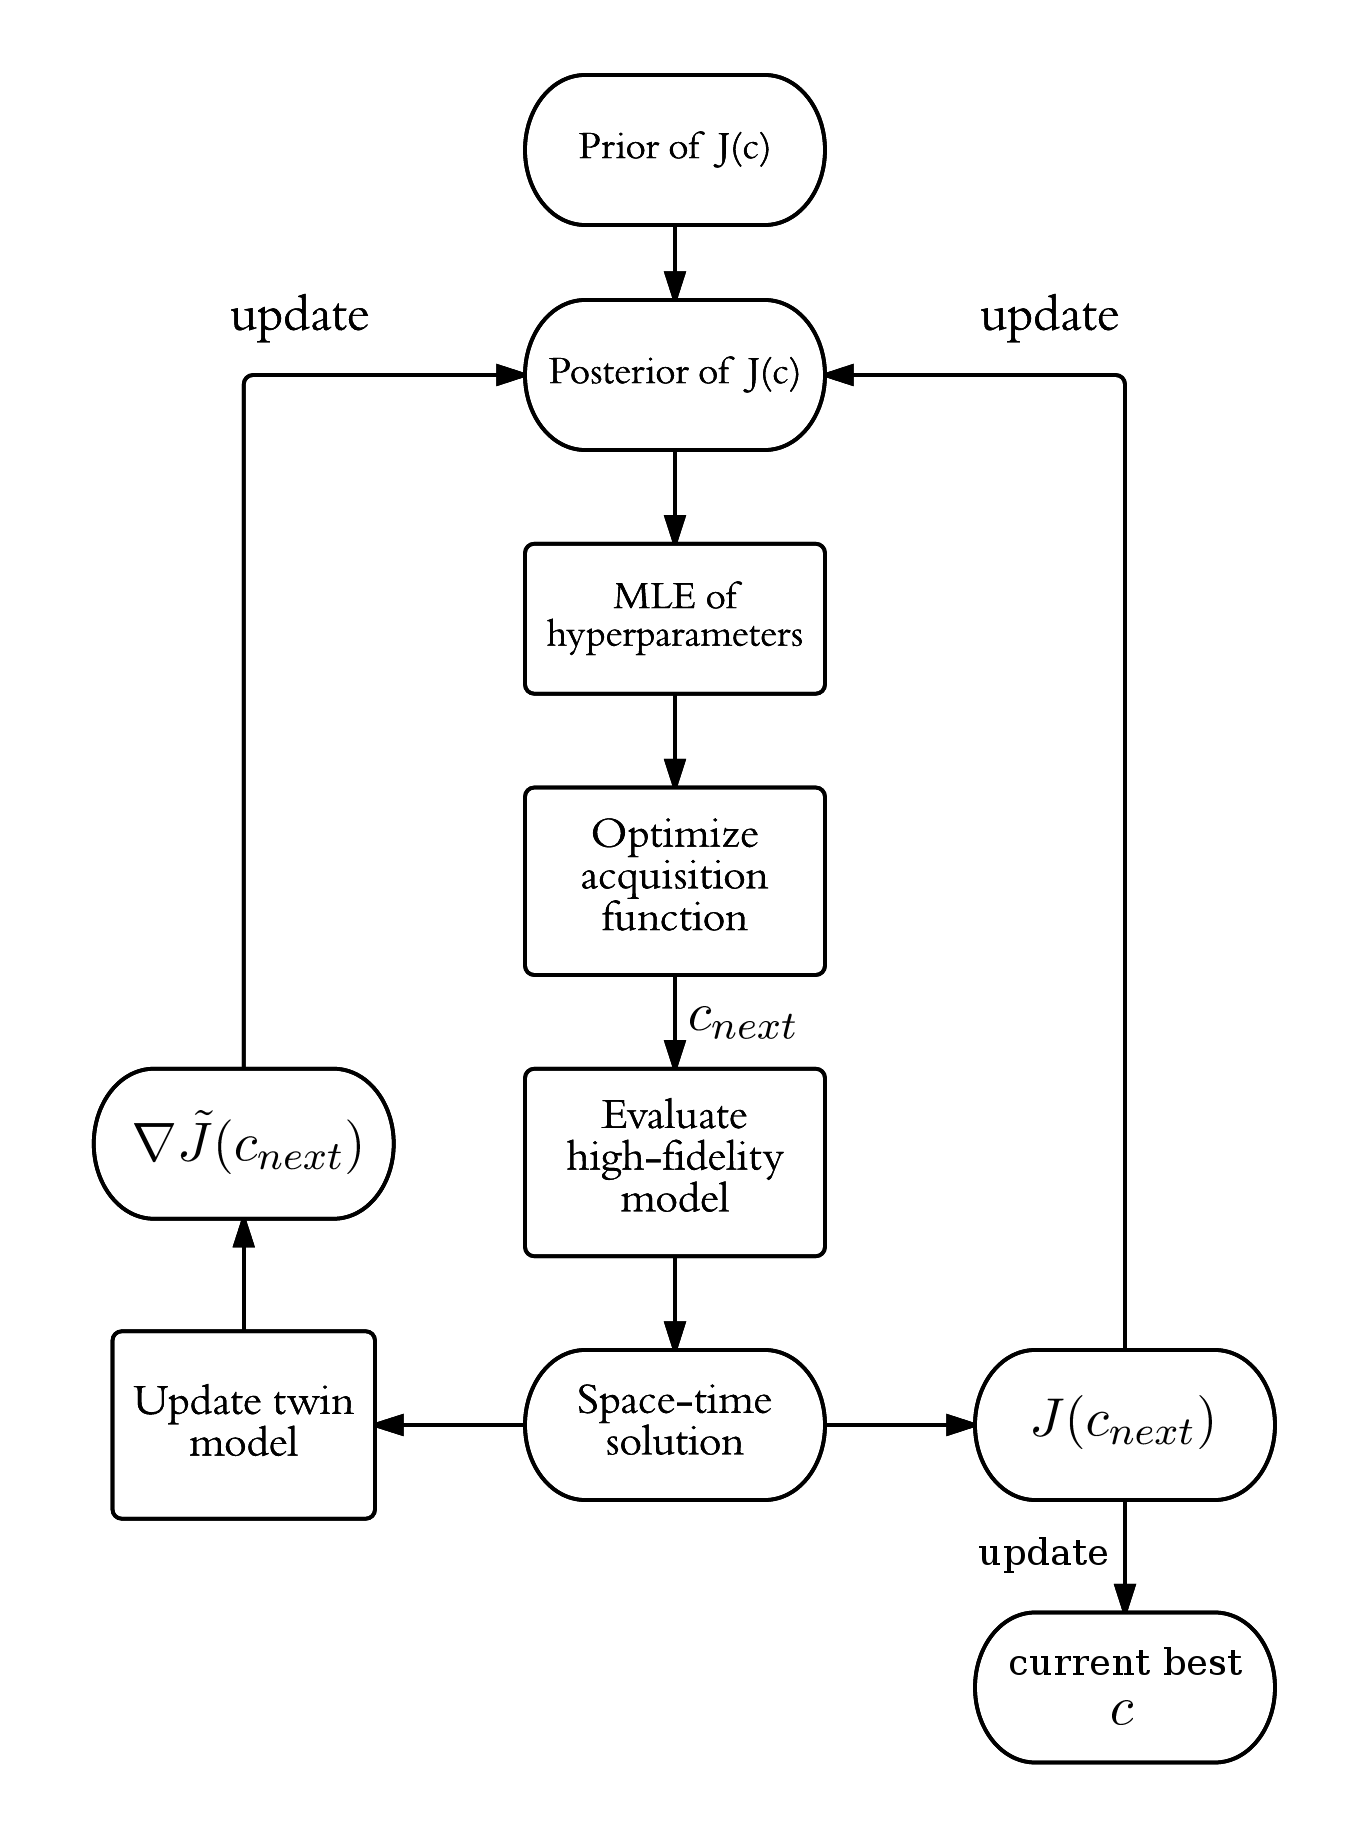
\includegraphics[height=12cm]{Bopt_flowchart.png}
        \caption{The flowchart of Bayesian optimization with twin model.}
        \label{fig: Bopt flow}
    \end{center}
\end{figure}

\noindent Intuitively, as the design space dimension increases, the ability to estimate 
$\frac{dJ}{dc}$ may become more important for faster $J$ reduction. 
For illustration, we consider minimizing
\begin{equation}
    J(x) = \sum_{i=1}^{\textrm{dim}} x_i^2\,.
\end{equation}
The true optimal is $x=\mathbf{0}$. Suppose the evaluation of $J$ is so expensive
that we can only evaluate it for 10 times. When $\textrm{dim}$ increases, we may expect
the smallest $J$ in the 10 evaluations to increase. When an estimation of $\frac{dJ}{dc}$
is available, the objective function may be reduced more quickly during the 10 evaluations,
even if the gradient estimation is noisy. We demonstrate  the superiority of using 
estimated gradient in Fig\ref{fig: dim and J}.
\begin{figure}[H]
    \begin{center}
        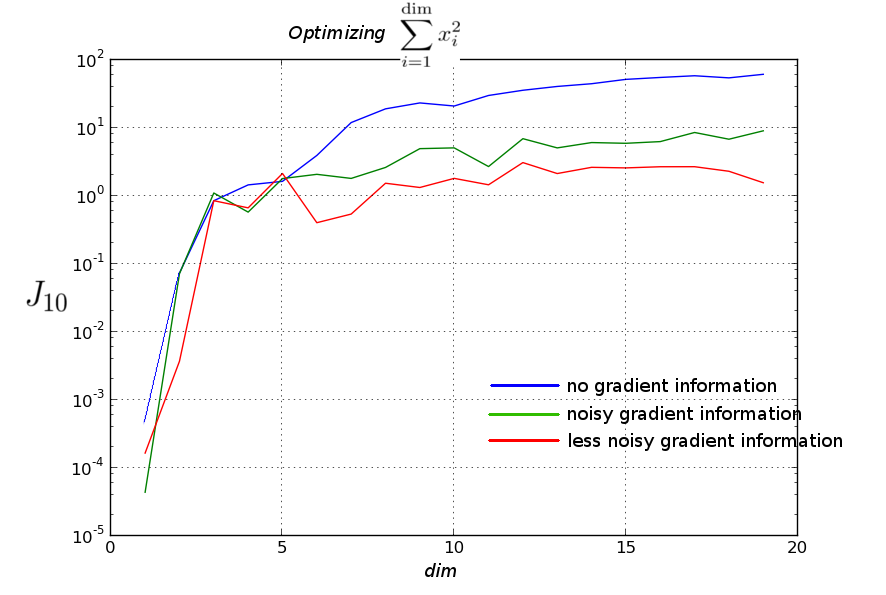
\includegraphics[height=7cm]{highdimoptdemon.png}
        \caption{Minimizing $J(x) = \sum_{i=1}^{\textrm{dim}}x_i^2$ with variable $\textrm{dim}$.
                 The y-axis is the best / smallest $J$ after 10 function evaluations, in log 10 scale.
                 The blue line is obtained from Bayesian optimization with no gradient information.
                 The green line is obtained from Bayesian optimization with a noisy gradient, by
                 setting $\sigma^2 = \sigma^2_\epsilon$, see Eqn\eqref{funkernel} 
                 and Eqn\eqref{noise kernel}. The red line is obtained from Bayesian optimization
                 with a less noisy gradient, by setting $0.1 \sigma^2 = \sigma^2_\epsilon$
                 We use Monte Carlo to randomly select some initial guesses for $x$. Each point
                 on these lines represents the averaged $J_{10}$ using a random set of 
                 initial guesses.}
        \label{fig: dim and J}
    \end{center}
\end{figure}

\subsection{Discussion of the convergence property}
\noindent Bayesian optimization is a deterministic global optimization strategy.
Given previous evaluations, it locates deterministically the next design point for evaluation. In the
end, the optimization generates an infinite sequence of design points.
Clearly, given an optimization strategy, 
the sequence depends on the underlying function to evaluate, and depends on the initial design.
The convergence property of Bayesian optimization can be discussed by the property of the design
sequence, using the following theorem \cite{Torn and Zilinskas}:\\
\fbox{\parbox{\textwidth}{
\begin{theorem}
    Let $W^{k,p}(\mathcal{X})$ be a Sobolev space of functions defined on $\mathcal{X}$.
    For any initial design in $\mathcal{X}$, 
    a global optimization algorithm converges for all functions in $W^{k,p}(\mathcal{X})$
    if and only if the design sequence produced by the algorithm is dense in $\mathcal{X}$
    for all functions in $W^{k,p}(\mathcal{X})$.
\end{theorem}
}}\\

\noindent Therefore, 
we will investigate whether the sequence produced by the proposed optimization scheme is dense.
If we can sample the exact function value, 
and if we use the expected improvement acquisition
function, it has been shown \cite{convergenceBayesian, Bayopt converge 2} the sequence is indeed dense,
under some mild conditions on the objective function.
In this section, we extend the theoretical result to sample both the exact function value and
noisy function gradient.\\
\fbox{\parbox{\textwidth}{
\begin{theorem}
    \textbf{The design sequence is dense.}\\
    Assume
    \begin{enumerate}
        \item $\mathcal{X} \in \mathbb{R}^n$, $\|\cdot\|$ be the $L_2$ norm defined on $\mathcal{X}$.
        \item $\mathcal{H}$ and $\mathcal{H}^\prime$ be two reproducing kernel Hilbert spaces 
              of functions
              on $\mathcal{X}$, with kernels $K(\cdot, \cdot): \mathcal{X}\times \mathcal{X}\mapsto
               \mathbb{R}$ and $K^\prime(\cdot, \cdot): \mathcal{X}\times \mathcal{X}\mapsto
               \mathbb{R}$ respectively.
        \item There exist $k: \mathbb{R}^+ \bigcup \{0\}\mapsto \mathbb{R}$ and 
              $k^\prime: \mathbb{R}^+ \bigcup\{0\}\mapsto \mathbb{R}$, such that
              $K$ and $K^\prime$ satisfies $K(x,y) = k(\|x-y\|)$ and
              $K^\prime(x,y) = k^\prime(\|x-y\|)$ respectively, for $\forall x, y
               \in \mathcal{X}$.
        \item $k$ and $k^\prime$ has the Fourier transforms $\hat{k}$
              and $\hat{k}^\prime$ respectively.  
              They satisfy the asymptotic properties
              $\hat{k}(u) = {\Theta}(|u|^{-n-2\nu})$ and 
              $\hat{k}^\prime(u) = {\Theta}(|u|^{-n-2\nu^\prime})\,,$ 
              as $|u|\rightarrow \infty$, with $\frac{1}{2}<\nu<\infty$ and $\nu^\prime = \nu-1$.
              ( $\Theta$ is the asymptotic big $\Theta$ notation. )
    \end{enumerate}
    Then all functions in $\mathcal{H}$ are differentiable.\\

    In addition, let 
    \begin{enumerate}
        \item $f\in \mathcal{H}$. 
        \item $\epsilon = \left(\epsilon_1,\cdots,\epsilon_n \right)^T\,, 
               \; \epsilon_i\in\mathcal{H}^\prime\;, i=1,\cdots,n$. 
              $\epsilon_i$ is independent of $\epsilon_j\;$ for $i\neq j$.
        \item $
                  g = \epsilon + \nabla f\,.
              $
    \end{enumerate}
    Suppose an infinitely long sequence is generated by the following strategy:
    \begin{equation*}\begin{split}
        x_{s+1} &= \arg\max_{x\in\mathcal{X}} \mathbb{E} \left[
        \max\left( f(x) -  f(x_s^*) ,0\right) \Big| \mathcal{S}
        \right]\\
        x_s^* &= \arg\max_{x\in\{x_1,\cdots,x_s\}}f(x)\\
        \mathcal{S} &= \Big\{ \left\{x_1,\cdots, x_s\right\} ,
        \left\{f(x_1),\cdots, f(x_s)\right\},
        \left\{g(x_1),\cdots, g(x_s)\right\}\Big\}
    \end{split}\end{equation*}
    Then the sequence $\left\{ x_1, x_2, \cdots \right\}$ 
    is dense in $\mathcal{X}$ for $\forall x_1\in \mathcal{X}$.
    \label{theorem: 2}
\end{theorem}
}}\\

\noindent As a future work, we will prove the theorem.


\subsection{Optimization constraints}
\label{constraints}
\noindent In the previous sections, we considered only non-constraint optimization for simplicity.
In order to deal with the more general formulation Eqn\eqref{general opt}, we
need to consider inequality constraint optimization. Inequality constraint optimization 
is of great interest in the engineering community. For example, in the design of
internal cooling ducts in turbomachineries, one possible objective is to minimize 
the pressure loss in a 180-degree return bend. However, reducing pressure loss may 
also reduce heat transfer, thus reduce the cooling ability
\cite{ubend rans opt 1, ubend rans opt 2}. Therefore, a viable approach is to set
a minimum heat transfer constraint while minimizing pressure loss. Another possible constraint
in the internal cooling duct problem is the geometric bound on the duct's wall.
This is because the duct must be contained 
inside the airfoil, and must be geometrically compatible with other components.
We illustrate such a constraint in Fig \ref{fig: simple constraint}.
\begin{figure}[H]
    \begin{center}
        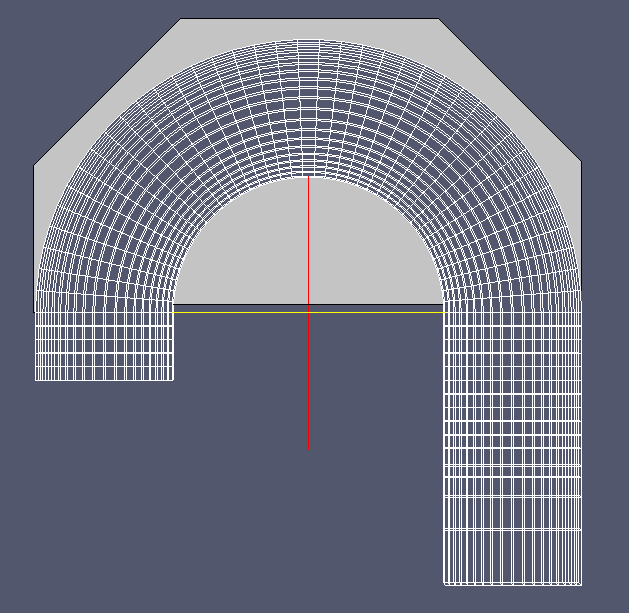
\includegraphics[height=6cm]{geometric_constraint.png}
        \caption{Example of a constraint of the feasible geometry, The brighter region indicates
                 feasible region of the return bend geometry. The wireframe indicates
                 a feasible design.}
        \label{fig: simple constraint}
    \end{center}
\end{figure}

\noindent Constraints can be categorized into two types based on how they are evaluated: 
the first type are constraints that require a PDE simulations's space-time solution;
the second type are constraints that do \emph{not} require the space-time solution.
In the example above, the constraint on the heat transfer belongs to the first type,
while the constraint on the duct geometry belongs to the second type.
Generally, evaluation of the first type constraint is much more expensive than
the second type constraint, and can be similarly expensive as the evaluation of the 
objective function.
Let the feasible region specified by the first type constraints be $\mathcal{C}_1$,
and let the feasible region specified by the second type constraints be $\mathcal{C}_2$.
The feasible region in Eqn\eqref{general opt} is $\mathcal{C} = \mathcal{C}_1 \bigcap
\mathcal{C}_2$.
\\

\noindent The second type constraints are not the topic of my research, because
generally they can be
evaluated cheaply. Optimization modules such as NLopt\cite{nlopt} have already
implemented many established methods for such constraints.
In Bayesian optimization, this type of constraints can be implemented in 
the optimization of the acquisition function, so the next evaluation point is always inside
$\mathcal{C}_2$.
The first type constraints, however, require special attention.
If we choose the expected improvement formulation in our Bayesian optimization,
Eqn\eqref{EI form} should be modified to:
\begin{equation}
    c_{s+1} = \arg\max_{c\in\mathcal{C}_2} \Big\{ \mathbb{E} 
    \left[\left. \max\left(J(c) - J(c^*_s), 0\right) \right.\Big| \mathcal{S}\right]\cdot
    \mathbb{P}\big[V(c)\le 0 \big| \mathcal{S}\big] \Big\}\,,
    \label{EI form constraint}
\end{equation}
The modified formulation is called \emph{constraint expected improvement}
\cite{constraint Bayesian Opt}.
Here $c_s^*$ is the best \emph{feasible} design in the previous $s$ iterations.
Notice the optimization domain is $c\in\mathcal{C}_2$.
Intuitively, improvement on $J$ is not counted valid unless the design is feasible.
\\

\noindent Similar to $J(c)$, we can construct a posterior distribution on $V(c)$ and
evaluate $\mathbb{P}\big[V(c)\le 0 \big| \mathcal{S}\big] $ in Eqn\eqref{EI form constraint}.
Straightforward evaluations of $V(c)$
using the primal model can be costly.
However, similar to $J(c)$, we can use the twin model to estimate the gradient of $V(c)$
cheaply. Specifically, we construct the posterior of $V(c)$
using evaluations of $V(c)$ and $\frac{d\tilde{V}(c)}{dc}$, and use
Eqn\eqref{EI form constraint} as our acquisition function to perform optimization.
The framework is shown in Fig \ref{fig: constraint bay opt}.
\begin{figure}[H]
    \begin{center}
        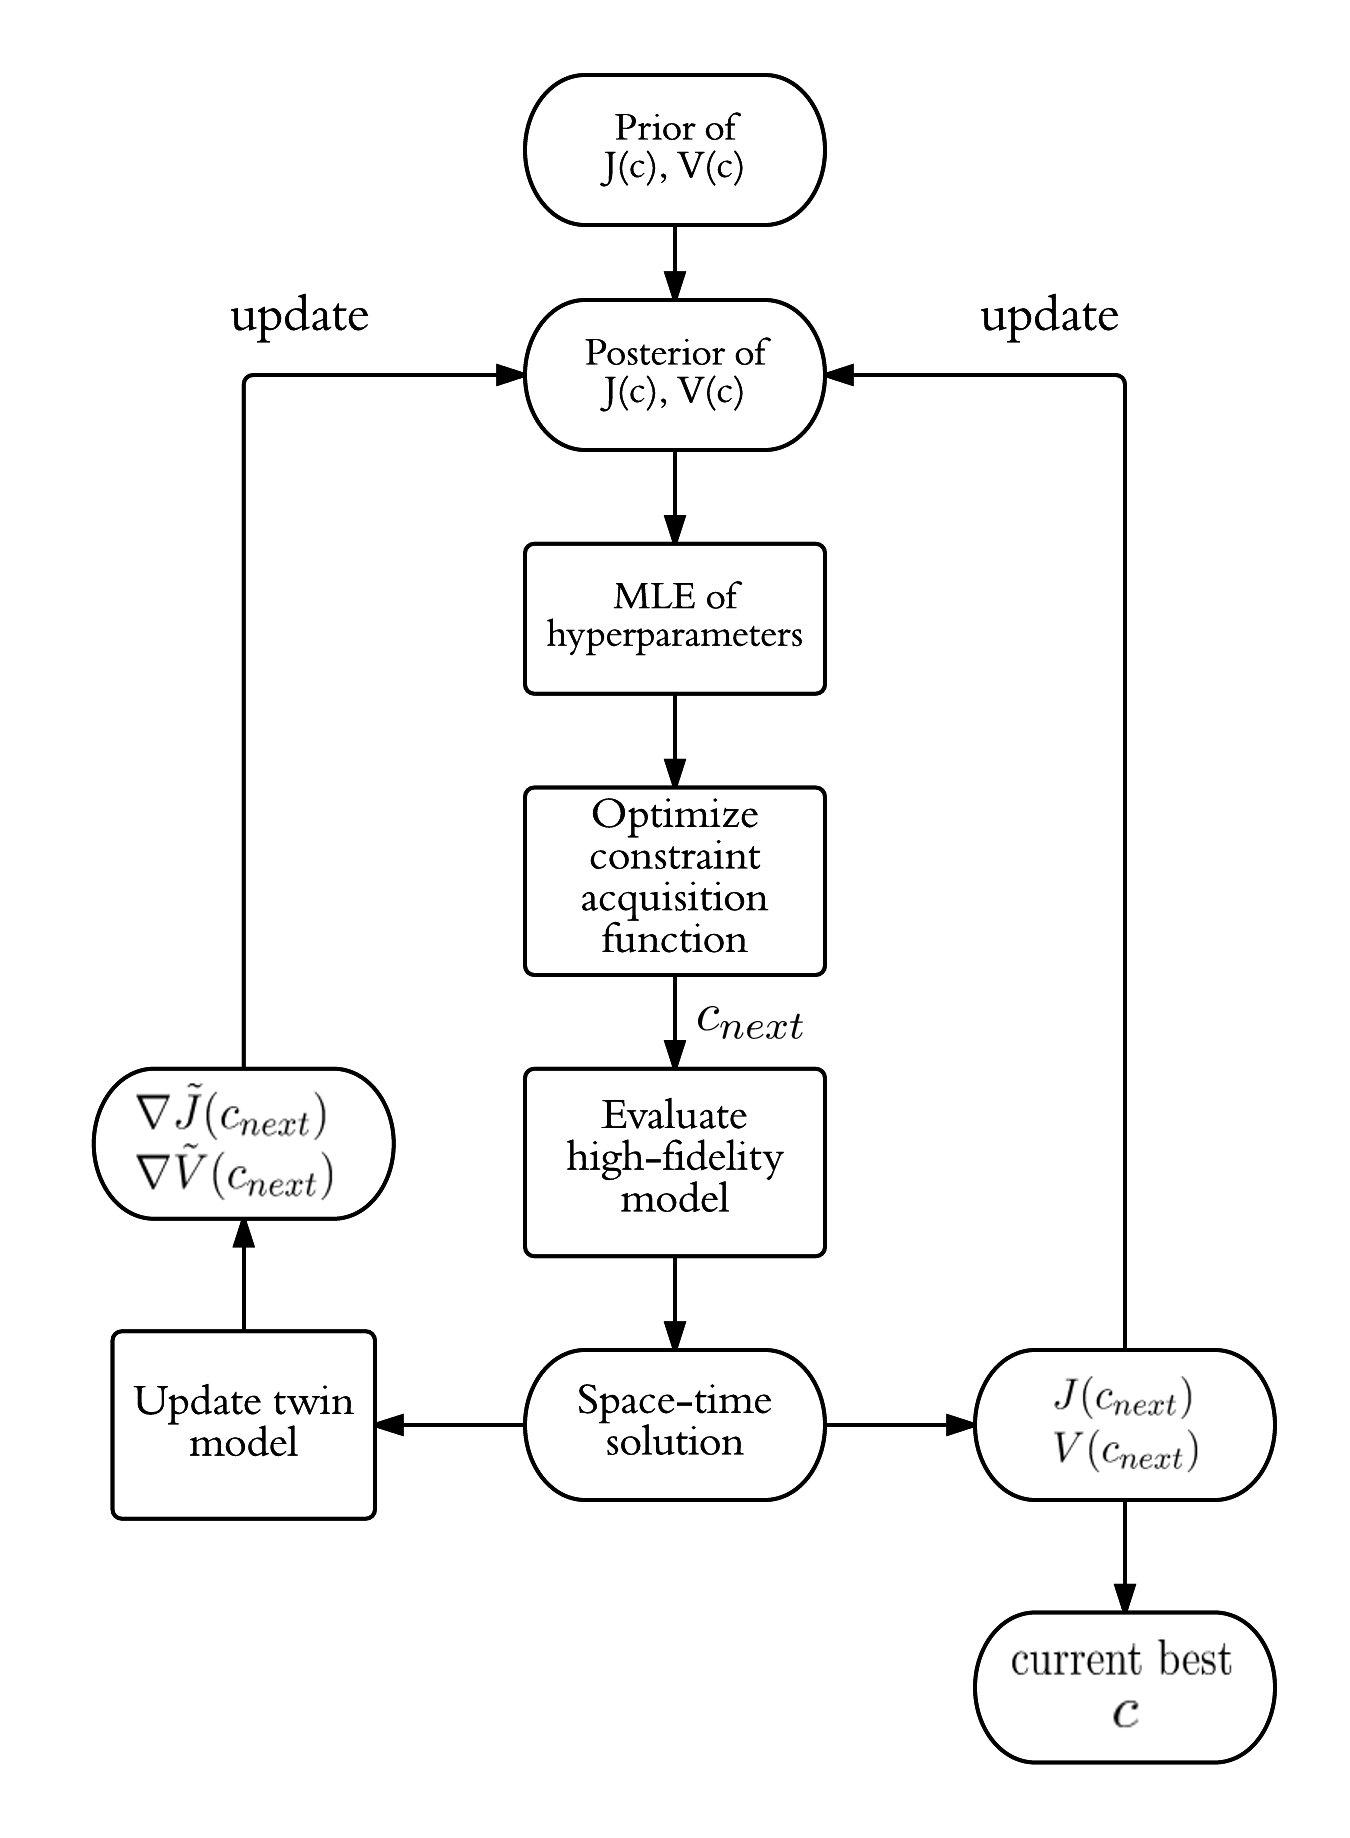
\includegraphics[height=12cm]{Bayconstraint.png}
        \caption{The flowchart of constraint Bayesian optimization with twin model.}
        \label{fig: constraint bay opt}
    \end{center}
\end{figure}



\newpage
\section{Application to a turbulent flow optimization}
\label{examples}
\subsection{Problem description}
\noindent Gas turbine blades are designed to operate at high temperatures. Because 
materials employed for turbine components may not withstand such high termperatures,
cooling should be applied to the blades for safety. A cooling method is
to drill tubes inside the blades to circulate the coolant air, shown in Fig\ref{fig: ubend picture}.
The pressure to drive the coolant flow is diverted from the compressor, thus resulting
in a penalty to the turbine efficiency.
An effective design should have minimal coolant flow rate and/or pressure drop penalty 
\cite{ubend rans opt 1, ubend rans opt 2}.
Generally, the cooling tube layout looks like a stack of several \emph{return bends}.
Therefore, some researchers consider optimizing the design of a single return bend
for simplicity. Optimization based on flow simulation have been employed to optimize
the return bend geometry. Generally such flow is turbulent, since the Reynolds number 
can be tens of thousands ($\sim$40,000 \cite{ubend rans opt 2}). 
Also, the flow may contain several complex
features, such as separation and reattachment, which are not captured well in the low-fidelity
simulations. Although a high-fidelity PDE model can be used to simulate the flow, 
the computational cost can be prohibitively expensive when the design space is high. 
\begin{figure}[H]\begin{center}
    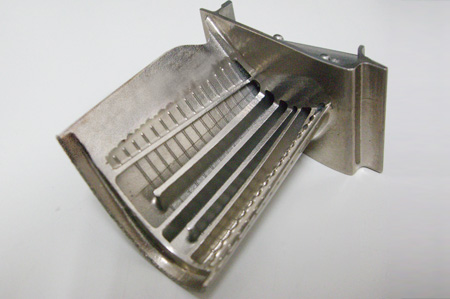
\includegraphics[height=5cm]{ubend.png}
    \caption{Example of turbine blade cooling tubes.
    Image from: \emph{http://www.amateras-tyo.biz/eng/technologies.html}}
    \label{fig: ubend picture}
\end{center}\end{figure}

\noindent Currently, adjoint method has not been implemented for high-fidelity PDE simulations
like DNS and LES. So efficient gradient evaluation of the high-fidelity PDE models 
are not available.
However, there are a set of low-fidelity models like RANS. 
RANS can be evaluated more cheaply; and adjoint can be implemented on RANS easily.
Because the high-fidelity simulations can provide
space-time solutions of all relevant flow quantities (velocity, pressure, etc), we consider
training RANS models using the time averged space-time solution of the high-fidelity simulation.
Therefore, we will consider high-fidelity models like LES a gray-box simulation,
and consider the trained RANS model a twin model.
Generally, the Mach number in such flows are low ($\sim$0.05 \cite{ubend rans opt 1}),
so we may focus on incompressible models. Besides, we will model the flow as two dimensional
for simplicity.
\\

\subsection{Review of incompressible RANS models}
\noindent RANS are time averaged equations of motion for fluid flow.
The idea behind the equation is Reynolds decomposition, where the flow instantaneous
quantities are decomposed into its time-averaged and fluctuating quantities.
For a stationary incompressible Newtonian fluid, the equations are
\begin{equation}\begin{split}
    \nabla\cdot \bar{\mathbf{u}} &= 0\\
    \rho \bar{\mathbf{u}}\cdot \nabla \bar{\mathbf{u}} &= -\nabla \bar{p} + \mu \nabla^2
    \bar{\mathbf{u}}
    -{\rho} \nabla \cdot\left(\overline{\mathbf{u}^\prime \mathbf{u}^\prime}\right)\,.
\end{split}\end{equation}
Here the instantaneous velocity $\mathbf{u} = (u,v)^T$ is decomposed as 
$\mathbf{u} = \bar{\mathbf{u}} + \mathbf{u}^\prime$. $\bar{\mathbf{u}}$ is the 
time-averaged velocity and $\mathbf{u}^\prime$ is the fluctuating velocity.
Similarly $p = \bar{p} + p^\prime$.
$\rho$ is the constant density, $\mu$ is the dynamic viscosity.
The term
\begin{equation}
    \mathbf{R} = \rho \overline{\mathbf{u}^\prime \mathbf{u}^\prime}
\end{equation}
is called \emph{Reynolds stress}.\\

\noindent Modelling the Reynolds stress is recognized as a closure problem, and
is a subject of intense interest for almost a century. 
There are many models for Reynolds stress, in which a popular class of 
models is based on the \emph{Boussinesq hypothesis} \cite{Wilcox CFD}.
Boussinesq hypothesis models the Reynolds stress by a linear constitutive relationship with
the mean flow straining field:
\begin{equation}
    \mathbf{R} = -\mu_t \left( \nabla \bar{\mathbf{u}} + \nabla \bar{\mathbf{u}}^T\right)
    + \frac{1}{3}\rho \bar{\mathbf{u}} \cdot \bar{\mathbf{u}} \boldsymbol{I}
\end{equation}
$\mu_t$ is called \emph{eddy viscosity}. 
$\nu_t = \mu_t/\rho$ is called \emph{kinematic eddy viscosity}.
The only term that needs to be modelled for closure is $\mu_t$ (or $\nu_t$).\\

\noindent Depending on how $\mu_t$ is modelled, most RANS models based
on Boussinesq hypothesis can be categorized in to three classes:
\emph{zero equation models}, \emph{one equation models}, and \emph{two equation models}.
Zero equation models do not require the solution of additional equations.
$\mu_t$ is calculated directly from \emph{local} flow variables. Therefore, zero
equation models may not be able to capture the phenomenons like convections and diffusions
of turbulent energy.
For example, a classical zero equation model is the Prandtl's mixing length model 
\cite{Wilcox CFD}:
\begin{equation}
    \mu_t = \rho \left| \frac{\partial u}{\partial y} \right| l_m^2\,,
    \label{Prandtl mixing length}
\end{equation}
where $\frac{\partial u}{\partial y}$ is the partial derivative of the streamwise velocity
with respect to the wall normal direction.
One equation models require the solution of one additional equation. Generally the additional
equation is a transport equation of a quantity related to the eddy viscosity.
For example, the Baldwin-Barth model \cite{Wilcox CFD} decomposes $\mu_t$ as
\begin{equation}
    \mu_t =  C_\mu\mu \tilde{R}_T D_1 D_2\,,
\end{equation}
where $C_\mu$ is a constant, $D_1$, $D_2$ are spatial-dependent variables, $\mu \tilde{R}_T$
is solved by a transport equation.
Two equation models require the solution of two additional equations. 
An example is the \emph{k-epsilon models}
\cite{Wilcox CFD}.
k-epsilon models assume the eddy viscosity to be
\begin{equation}
    \mu_t = C_\mu \frac{k^2}{\epsilon}\,,
\end{equation}
where
\begin{equation}\begin{split}
    k = \frac{\bar{u^\prime}^2 + \bar{v^\prime}^2 }{2}
\end{split}\end{equation}
is the \emph{turbulent kinetic energy},
\begin{equation}
    \epsilon = \nu \overline{ 
    \left(\nabla\mathbf{u}^\prime\right) :\left( \nabla\mathbf{u}^\prime \right)^T}
\end{equation}
is the \emph{turbulent dissipation rate}, 
and $C_\mu$ is a constant.
k-epsilon models solve two transport equations for $k$ and $\epsilon$.
Generally, two-equation models are better at capturing some turbulent flow features
such as convection and diffusion of turbulent energy, detachment, and reattachment
\cite{Wilcox CFD}.
\\

\subsection{Future work}
\noindent We will optimize the return bend geometry to minimize the pressure loss using the
proposed optimization framework. We may parameterize the return bend
geometry by a set of \emph{design nodes} on the inner and outter boundaries, 
and use a spline interpolation to generate the
boundaries. The dimension of the design space will be the number of design nodes.
We will use tens of design nodes, which yields a challenging high-dimensional optimization problem.
There have been researches on this topic both numerically and experimentally
\cite{ubend rans opt 1, ubend rans opt 2}. These researches can benchmark our results.
However, instead of optimizing for the low-fidelity model's
optimal which was the practice of most previous researches,
we aim at optimizing for the high-fidelity model's optimal.\\

\noindent We will implement an LES model in OpenFoam to serve as the high-fidelity gray-box 
simulation; and implement a one-equation or two-equation RANS model in python to
serve as the low-fidelity twin model. We will implement adjoint in the RANS model, using
an automatic differentiation toolbox.
In the RANS model, the equation(s) of the eddy viscosity will be adaptive.
Further investigation is required to find appropriate forms of the adaptive 
eddy viscosity equation(s), and to adaptively select the basis for the eddy viscosity equation(s). 
After that, we will train the adaptive RANS model with the LES' time-averaged 
space-time solution. Then we can use the proposed Bayesian optimization framework 
to perform optimization. In the end, 
we will survey state-of-art designs in literatures, and compare them with
our optimal design, using LES simulation.\\



\newpage
%\begin{appendices}
\section{Appendices}
    \subsection{Proof of theorem \ref{theorem: 1}: global-local error}
    \label{appendix 1}
    \emph{Proof:} Consider a primal model and a twin model solving
    for the space-time solution $u$ and $\tilde{u}$ on the same
    time grid $\{t_0=0,t_1,\cdots, t_n=T\}$. The solutions at timestep $t_i$
    are $u_i$ and $\tilde{u}_{i}$. Both simulations 
    starts from the same initial condition $u_0$. Define the mapping
    of the primal model 
    \begin{equation}
        H:\, \mathbb{R}^n\mapsto\mathbb{R}^n,\, u^i\rightarrow Hu^i = u^{i+1}\,,
        \quad i=1,\cdots, n
    \end{equation}
    and the mapping of the twin model
    \begin{equation}
        G:\, \mathbb{R}^n\mapsto\mathbb{R}^n,\, \tilde{u}^i\rightarrow 
        G\tilde{u}^i = \tilde{u}^{i+1}\,,\quad i=1,\cdots, n
    \end{equation}
    $G$ and $H$ are linear or nonlinear mappings.
    We illustrate these mappings in Fig \ref{fig:sketch}.
    \begin{figure}[H]\begin{center}
        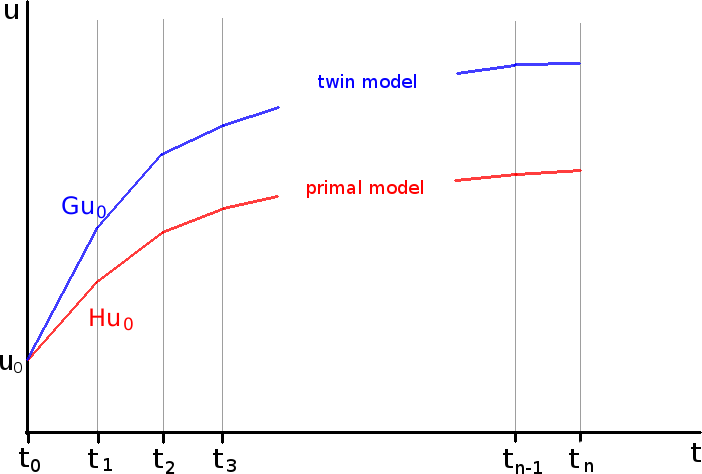
\includegraphics[height=5cm]{sketch.png}
        \caption{Trajectories of the primal model and the twin model. 
                 $H$ and $G$ are their timestep-wise mapping functions.}
        \label{fig:sketch}
    \end{center}\end{figure}
    \noindent The global error is
    \begin{equation}
        Err_G = \frac{1}{n\Delta t}\left\{ \|(G^n - H^n) u_0\| + \|(G^{n-1}-H^{n-1})u_0\|
        +\cdots+\|(G^1-H^1)u_0\| \right\}
        \label{global error}
    \end{equation}
    The local error is
    \begin{equation}
        Err_L = \frac{1}{n\Delta t} \left\{
            \|\left(GH^{n-1} - H^{n}\right)u_0\| +  
            \|\left(GH^{n-2} - H^{n-1}\right)u_0\| + \cdots +
            \|\left(G^1-H^1\right)u_0\|
        \right\}
        \label{local error}
    \end{equation}
    Using the equality
    \begin{equation}
        G^i-H^i = (G^i-G^{i-1}H) + (G^{i-1}H - G^{i-2}H^2) + \cdots + (GH^{i-1}-H^i)\,,\quad
        i\in \mathbb{Z}^+\,,
    \end{equation}
    we derive from Eqn\eqref{global error}
    \begin{equation}
        Err_G \le \frac{1}{n\Delta t}
        \left\{\begin{split}
            \|(G^{n-1} G - G^{n-1}H)u_0\| &+ \|(G^{n-2}GH - G^{n-2}H^2)u_0\|&+\cdots
            &+ \|(GH^{n-1} - H^{n})u_0\|\\
            &+\|(G^{n-2} G - G^{n-2}H)u_0\| &+ \cdots 
            &+ \|(GH^{n-2} - H^{n-1})u_0\|\\
            &\ddots&& \vdots\\
            &&& + \|(G - H)u_0\|
        \end{split}
        \right\}
        \label{expansion global error}
    \end{equation}
    Using Eqn\eqref{expansion global error} and Eqn\eqref{local error}, we get
    \begin{equation}
        Err_G - Err_L \le 
        \frac{1}{n\Delta t}
        \left\{\begin{split}
            \|(G^{n-1} G - G^{n-1}H)u_0\| &+ \|(G^{n-2}GH - G^{n-2}H^2)u_0\|&+\cdots
            &+ \|(GGH^{n-2} - G H^{n-1})u_0\|\\
            &+\|(G^{n-2} G - G^{n-2}H)u_0\| &+ \cdots 
            &+ \|(GGH^{n-3} - G H^{n-2})u_0\|\\
            &\ddots&& \vdots\\
            &&& + \|(G G - G H)u_0\|
        \end{split}
        \right\}
        \label{error diff}
    \end{equation}
    Apply our assumption
    \begin{equation}
        \left\| Gx - Gy \right\| \le \alpha \|x-y\|
    \end{equation}
    and its implication
    \begin{equation}
        \left\|G^i x - G^i y\right\| \le \alpha^i \|x-y\|\,, \quad i\in \mathbb{Z}^+
    \end{equation}
    to Eqn\eqref{error diff}, we get
    \begin{equation}
        Err_G - Err_L \le 
        \frac{1}{n\Delta t}
        \left\{\begin{split}
            \alpha^{n-1}\|(G - H)u_0\| &+ \alpha^{n-2}\|(GH - H^2)u_0\|&+\cdots
            &+ \alpha\|(GH^{n-2} - H^{n-1})u_0\|\\
            &+\alpha^{n-2}\|( G - H)u_0\| &+ \cdots 
            &+ \alpha\|(GH^{n-3} - H^{n-2})u_0\|\\
            &\ddots&& \vdots\\
            &&& + \alpha\|(G - H)u_0\|
        \end{split}
        \right\}
        \label{error diff}
    \end{equation}
    Reorder the summation, we get
    \begin{equation}
        Err_G - Err_L \le 
        \frac{1}{n\Delta t}
        \left\{\begin{split}
            \alpha^{n-1}\|(G - H)u_0\| &+ \alpha^{n-2}\|(G - H)u_0\|&+\cdots
            &+ \alpha\|(G - H)u_0\|\\
            &+\alpha^{n-2}\|( GH - H^2)u_0\| &+ \cdots 
            &+ \alpha\|(GH - H^{2})u_0\|\\
            &\ddots&& \vdots\\
            &&& + \alpha\|(GH^{n-2} - H^{n-1})u_0\|
        \end{split}
        \right\}
        \label{error diff 2}
    \end{equation}
    Therefore, from Eqn\eqref{error diff 2} and Eqn\eqref{local error}, we get
    \begin{equation}
        Err_G \le (1+\alpha+\cdots+\alpha^{n-1}) Err_L\,.
    \end{equation}
    If $|\alpha|$ is strictly less than $1$, 
    \begin{equation}
        Err_G \le \frac{1}{1-\alpha} Err_L\,,
    \end{equation}
    which completes the proof.$\hfill\Box$

%    \section{Proof of theorem \ref{theorem: 2}: gradient of twin model}
%    What to prove: If the twin model flux and rhs is close to the primal model,
%    then the gradients are close. Intermediate step, the adjoint state are close.
%    Consider objective function $\int_t\int_{\Omega} J(u,c)$.
%    The adjoint satisfies
%    \begin{equation}
%        \frac{\partial \lambda}{\partial t} + \nabla F(u)\cdot \nabla\lambda
%        = \frac{\partial J}{\partial u} - \frac{\partial q}{\partial u}\lambda
%    \end{equation}
%    with $\lambda(T) = 0$ and $\lambda\big|_{\partial \Omega} = 0$.\\
%    Need to show: if $\|F_1-F_2\|$ and $\|q_1-q_2\|$ are bounded, then
%    $\|\lambda_1-\lambda_2\|$ is bounded.


%    \section{Proof of theorem \ref{theorem: 2}: design sequence is dense}
%    \label{proof convergence append}
%    To be proven.


%\end{appendices}

\newpage
\begin{thebibliography}{9}
\bibitem{hanmaster} 
Han Chen.
"Blackbox stencil interpolation method for model reduction"
Master thesis, 2012

\bibitem{Han AIAA} 
Chen, Han, et al. 
"Conditional sampling and experiment design for quantifying manufacturing error of transonic airfoil." 
Proceedings of the 49th Aerospace Sciences Meeting. 2011.

\bibitem{Active subspace}
Constantine, Paul G., Eric Dow, and Qiqi Wang. 
"Active subspace methods in theory and practice: Applications to kriging surfaces." 
SIAM Journal on Scientific Computing 36.4 (2014): A1500-A1524.

\bibitem{Balanced truncation}
Willcox, Karen, and Jaime Peraire. 
"Balanced model reduction via the proper orthogonal decomposition." 
AIAA journal 40.11 (2002): 2323-2330.

\bibitem{andrewras}
March, Andrew, Karen Willcox, and Qiqi Wang. 
"Gradient-based multifidelity optimisation for aircraft design using Bayesian model calibration." 
Aeronautical Journal 115.1174 (2011): 729.

\bibitem{jones1998}
Jones, Donald R., Matthias Schonlau, and William J. Welch. 
"Efficient global optimization of expensive black-box functions." 
Journal of Global optimization 13.4 (1998): 455-492.

\bibitem{convergenceBayesian}
Bull, Adam D. 
"Convergence rates of efficient global optimization algorithms." 
The Journal of Machine Learning Research 12 (2011): 2879-2904.

\bibitem{NARMAXbook}
Stephen A Billings.
"Nonlinear System Identification, NARMAX methods in time, frequency and spatial-temporal domains"
ISBN:978-1-119-94359-4, 2013

\bibitem{practicalBayesianopt}
Snoek, Jasper, Hugo Larochelle, and Ryan P. Adams. 
"Practical Bayesian optimization of machine learning algorithms." 
Advances in Neural Information Processing Systems. 2012.

\bibitem{KennedyOhagan1}
Kennedy, Marc C., and Anthony O'Hagan. 
"Predicting the output from a complex computer code when fast approximations are available." 
Biometrika 87.1 (2000): 1-13.

\bibitem{KennedyOhagan2}
A. O'Hagan 
"A Markov property for covariance structures." 
Nottingham University Statistics Research Report 13 (1998).

\bibitem{MCMC hyperparameters}
Murray, Iain, and Ryan P. Adams. 
"Slice sampling covariance hyperparameters of latent Gaussian models." 
Advances in Neural Information Processing Systems. 2010.

\bibitem{Krigingold}
Oliver, Margaret A., and R. Webster. 
"Kriging: a method of interpolation for geographical information systems." 
International Journal of Geographical Information System 4.3 (1990): 313-332.

\bibitem{inexactgradient1}
Carter, Richard G. 
"Numerical experience with a class of algorithms for nonlinear optimization using inexact function and gradient information." 
SIAM Journal on Scientific Computing 14.2 (1993): 368-388.

\bibitem{inexactnewton1}
Dembo, Ron S., Stanley C. Eisenstat, and Trond Steihaug. 
"Inexact newton methods." 
SIAM Journal on Numerical analysis 19.2 (1982): 400-408.

\bibitem{trustregionconn}
Conn, Andrew R., Katya Scheinberg, and Luís N. Vicente. 
"Global convergence of general derivative-free trust-region algorithms to first-and second-order critical points." 
SIAM Journal on Optimization 20.1 (2009): 387-415.

\bibitem{trustregionwild}
Wild, Stefan M., and Christine Shoemaker. 
"Global convergence of radial basis function trust-region algorithms for derivative-free optimization." 
SIAM Review 55.2 (2013): 349-371.

\bibitem{kriging}
G.M. Matheron,
"Principles of geostatistics".
Economic Geology 58.8 (1963): 1246-1266

\bibitem{cokriging}
Goovaerts, Pierre. 
"Ordinary cokriging revisited." 
Mathematical Geology 30.1 (1998): 21-42.

\bibitem{bishopbook}
Christopher M. Bishop
Pattern recognition and machine learning
ISBN: 978-0387310732. 2007

\bibitem{SarmaEKF}
Sarma, Pallav, LJ Durlofsky, K Aziz, WH Chen. 
"Efficient real-time reservoir management using adjoint-based optimal control and model updating." 
Computational Geosciences 10.1 (2006): 3-36.

\bibitem{gradfreereview}
Rios, Luis Miguel, and Nikolaos V. Sahinidis. 
"Derivative-free optimization: A review of algorithms and comparison of software implementations." 
Journal of Global Optimization 56.3 (2013): 1247-1293.

\bibitem{dynamicprogramming}
Powell, Warren B.
"Approximate Dynamic Programming: Solving the curses of dimensionality".
Vol. 703. John Wiley \& Sons, 2007.

\bibitem{quasiNewton}
Dennis, Jr, John E., and Jorge J. Moré. 
"Quasi-Newton methods, motivation and theory." 
SIAM review 19.1 (1977): 46-89.

\bibitem{adjoint}
Plessix, R-E. 
"A review of the adjoint-state method for computing the gradient of a functional with geophysical applications." 
Geophysical Journal International 167.2 (2006): 495-503.

\bibitem{cont discretize adjoint}
Nadarajah, Siva, and Antony Jameson. 
"A comparison of the continuous and discrete adjoint approach to automatic aerodynamic optimization." 
AIAA paper 667 (2000): 2000.

\bibitem{automaticdiff}
A Griewank, GF Corliss
Automatic differentiation of algorithms: theory, implementation, and application.
Defense Technical Information Center, 1992.

\bibitem{reservoir simulation book}
Zhangxin Chen
"Reservoir Simulation: Mathematical Techniques in Oil Recovery"
Society for Industrial and Applied Mathematics, ISBN 0898716403, 2007

\bibitem{wavelet mallat}
Mallat, Stephane G. 
"A theory for multiresolution signal decomposition: the wavelet representation." 
Pattern Analysis and Machine Intelligence, IEEE Transactions on 11.7 (1989): 674-693.

\bibitem{Bayopt converge 2}
Vazquez, Emmanuel, and Julien Bect. 
"Convergence properties of the expected improvement algorithm with fixed mean and covariance functions." 
Journal of Statistical Planning and inference 140.11 (2010): 3088-3095.

\bibitem{Buckley Leverett}
S.E. Buckley and M.C. Leverett
"Mechanism of fluid displacement in sands."
Transactions of the AIME 146 (1942): 107-116

\bibitem{Reservoir Simulation Book}
Chen, Zhangxin, Guanren Huan, and Yuanle Ma. 
"Computational methods for multiphase flows in porous media."
Vol. 2. Siam, 2006.

\bibitem{Boyd optimization}
Stephen Boyd and Lieven Vandenberghe
"Convex Optimization"
Cambridge University Press, 2004

\bibitem{Sigmoid Approximation}
G. Cybenko
"Approximation by superpositions of a sigmoid function"
Mathematics of control, signals and systems 2.4 (1989): 303-314

\bibitem{haar}
Alfred Haar
"On the theory of orthogonal function systems"
Mathematische Annalen 69 (1910): 331-371

\bibitem{Analytic Meyer}
V.VV. Vermehren, H.M. de Oliveira
"Close expressions for Meyer wavelet and scale function"
arXiv:1502.00161 [stat.ME]

\bibitem{Opt Koziel Book}
Slawomir Koziel, Xin-She Yang
"Computational optimization, methods and algorithms"
Springer Berlin Heidelberg, 2011

\bibitem{Surrogate based analysis and optimization}
N.V. Queipo, R.T. Haftka, W. Shyy, T. Goel, R. Vaidynathan, P.K Tucker
"Surrogate-based analysis and optimization"
Progress in Aerospace Sciences 41 (2005): 1-28

\bibitem{Space mapping 1}
T.D. Robinson, M.S. Eldred, K.E. Willcox, R. Haimes
"Surrogate-based optimization using multifidelity models with variable 
parameterization and corrected space mapping"
AIAA Journal 46 (2008): 2814-2822

\bibitem{Space mapping 2}
Mohamed H. Bakr, John W. Bandler
"An introduction to the space mapping technique"
Optimization and Engineering 2 (2011): 369-384

\bibitem{simplified physics}
N.M. Alexandrov, E.J. Nielsen, R.M. Lewis, W.K. Anderson
"First-Order Model Management with Variable-Fidelity Physics 
Applied to Multi-Element Airfoil Optimization"
8th AIAA Symposium on Multidisciplinary Design and Optimization (2000)

%\bibitem{equality nonlinear constraint trust region opt}
%Conn, Andrew R., Nicholas IM Gould, and Philippe Toint. 
%"A globally convergent augmented Lagrangian algorithm for optimization with general constraints and simple bounds."
%SIAM Journal on Numerical Analysis 28.2 (1991): 545-572.

\bibitem{coarse discretization}
N.M. Alexandrov, R.M. Lewis, C.R. Gumbert, L.L. Green, P.A. Newmann
"Optimization with Variable-Fidelity Models Applied to Wing Design"
38th Aerospace Sciences Meeting (2000)

\bibitem{gradient kriging surrogate}
Han Zhong-Hua, Stefan Görtz, Ralf Zimmermann
"Improving variable-fidelity surrogate modeling via gradient-enhanced kriging and a generalized hybrid bridge function."
Aerospace Science and Technology 25.1 (2013): 177-189.

\bibitem{poly functional surrogate}
Gary G. Wang, S. Shan
"Review of metamodeling techniques in support of engineering design optimization."
Journal of Mechanical Design 129.4 (2007): 370-380.

\bibitem{kriging functional surrogate}
Shinkyu Jeong, Mitsuhiro Murayama, Kazuomi Yamamoto
"Efficient optimization design method using kriging model" 
Journal of aircraft 42.2 (2005): 413-420.

\bibitem{ann functional surrogate}
Nestor V. Queipo, Javier V. Goicochea, Salvador Pintos. 
"Surrogate modeling-based optimization of SAGD processes." 
Journal of Petroleum Science and Engineering 35.1 (2002): 83-93.

\bibitem{adjoint gradient cokriging without MLE}
Hyoung-Seog Chung, Juan J. Alonso. 
"Using gradients to construct cokriging approximation models for high-dimensional design optimization problems." 
AIAA paper 317 (2002): 14-17.

\bibitem{survey of high dimensional blackbox optimization}
Songqing Shan, G. Gary Wang. 
"Survey of modeling and optimization strategies to solve high-dimensional design problems with computationally-expensive black-box functions." 
Structural and Multidisciplinary Optimization 41.2 (2010): 219-241.

\bibitem{review of black-box modeling}
Jonas Sjöberg et al.
"Nonlinear black-box modeling in system identification: a unified overview." 
Automatica 31.12 (1995): 1691-1724.

\bibitem{dimensional reduction}
Laurens JP van der Maaten, Eric O. Postma, H. Jaap van den Herik
"Dimensionality reduction: A comparative review." 
Journal of Machine Learning Research 10.1-41 (2009): 66-71.

\bibitem{decomposition}
T.R. Browning
"Applying the design structure matrix to system decomposition and integration problems: a review
 and new directions"
IEEE Trans Eng Manage 48.3 (2001): 292-306

\bibitem{variable selection}
Raymond H. Myers, Douglas C. Montgomery, Christine M. Anderson-Cook
"Response surface methodology: process and product optimization using designed experiments"
Vol. 705. John Wiley and Sons, 2009

\bibitem{thin airfoil}
Ira H. Abbott, E. Albert Von Doenhoff
"Theory of wing sections"
Dover Publications Inc., Section 4.2 (1959)

\bibitem{turbulent modeling R high}
Tsan-Hsing Shih, et al. 
"A new k-ϵ eddy viscosity model for high reynolds number turbulent flows" 
Computers and Fluids 24.3 (1995): 227-238.

\bibitem{turbulent modeling R low}
Virendra C. Patel, Wolfgang Rodi, and Georg Scheuerer
"Turbulence models for near-wall and low Reynolds number flows-a review"
AIAA journal 23.9 (1985): 1308-1319

\bibitem{NP hard}
Toby S. Cubitt, Jens Eisert, Michael M. Wolf
"Extracting dynamical equations from experimental data is NP hard"
Physical review letters 108.12 (2012): 120503

\bibitem{Hamilton Fluid Dynamics}
Rick Salmon 
"Hamiltonian fluid mechanics"
Annual review of fluid mechanics 20.1 (1988): 225-256

\bibitem{numerical schemes for hyperbolic equation review}
Randall J. LaVeque
"Finite volume methods for hyperbolic problems"
Vol. 31. Cambridge university press, 2002

\bibitem{SI old}
Pieter Eykhoff
"System identification, parameter and system estimation"
John Wiley and Sons, 1974

\bibitem{piecewise linear}
S.A. Billings, W.S.F Voon
"Piecewise linear identification of non-linear system"
International Journal of Control, 46.1 (1987): 215-235

\bibitem{volterra 1}
Georgios B. Giannakis, Erchin Serpedin
"A bibliography on nonlinear system identification"
Signal Processing 81.3 (2001): 533-580

\bibitem{volterra 2}
M.J. Korenberg, I.W. Hunter
"The Identification of Nonlinear Biological Systems: Volterra Kernel Approaches"
Annals Biomedical Engineering 24.2 (1996): 250-268

\bibitem{cross correlation}
Julian Jakob Bussgang
"Crosscorrelation functions of amplitude-distorted Gaussian signals" 
(1952)

\bibitem{feedback linear}
C.P. Kwong, C. F. Chen
"Linear feedback system identification via block-pulse functions"
International Journal of Systems Science 12.5 (1981): 635-642

\bibitem{billings 1981}
S.A. Billings, I.J. Leontaritis
"Identification of nonlinear systems using parametric estimation techniques"
Proceedings of the IEE Conference on Control and its Application, Warwick, UK, pp.183-187

\bibitem{ANN SI}
Sheng Chen, S. A. Billings, P. M. Grant
"Non-linear system identification using neural networks" 
International journal of control 51.6 (1990): 1191-1214

\bibitem{Wavelet SI}
Stephen A. Billings, Hua-Liang Wei
"A new class of wavelet networks for nonlinear system identification."
Neural Networks, IEEE Transactions on 16.4 (2005): 862-874.

\bibitem{correlation model validation}
S. A. Billings, W. S. F. Voon
"Correlation based model validity tests for non-linear models"
International Journal of Control 44.1 (1986): 235-244.

\bibitem{Dijkema book}
Tammo Jan. Dijkema
"Adaptive tensor product wavelet methods for solving PDEs"
PhD thesis, Utrecht University (2009)

\bibitem{simple opt}
Ismail Kucuk,  Ibrahim Sadek
"An efficient computational method for the optimal control problem for the Burgers equation." 
Mathematical and computer modelling 44.11 (2006): 973-982.

\bibitem{numpad}
Qiqi Wang,
Numpad package,
https://github.com/qiqi/numpad.git

\bibitem{sklearn}
Scikit-learn package,
https://github.com/scikit-learn/scikit-learn.git

\bibitem{nlopt}
Steven G. Johnson,
The NLopt nonlinear-optimization package, 
http://ab-initio.mit.edu/nlopt

\bibitem{Quasi-Newton Review}
John E. Dennis, Jorge J. Moré.
"Quasi-Newton methods, motivation and theory." SIAM review 19.1 (1977): 46-89.

\bibitem{Eric master thesis}
Eric Alexander. Dow,
"Quantification of structural uncertainties in RANS turbulence models."
Dissertation, Massachusetts Institute of Technology, 2011.

\bibitem{LBFGS}
J. Nocedal.
"Updating quasi-Newton matrices with limited storage"
Mathematics of Computation, 35 (1980): 773-782

\bibitem{review dimensional reduction}
Van der Maaten, Laurens JP, Eric O. Postma, and H. Jaap van den Herik. 
"Dimensionality reduction: A comparative review." 
Journal of Machine Learning Research 10.1-41 (2009): 66-71.

\bibitem{review variable selection}
Havi, Ron, and George H. John. 
"Wrappers for feature subset selection."
Artificial intelligence 97.1 (1997): 273-324.

\bibitem{Billing feature selection}
Wei, Hua-Liang, and Stephen A. Billings. 
"Feature subset selection and ranking for data dimensionality reduction." 
Pattern Analysis and Machine Intelligence, IEEE Transactions on 29.1 (2007): 162-166.

\bibitem{PCA review}
Jolliffe, Ian. Principal component analysis. John Wiley and Sons, Ltd, 2002.

\bibitem{constraint Bayesian Opt}
Gardner, Jacob, et al. 
"Bayesian optimization with inequality constraints."
Proceedings of The 31st International Conference on Machine Learning. 2014.

\bibitem{Lasso variable selection}
Tibshirani, Robert. 
"Regression shrinkage and selection via the lasso." 
Journal of the Royal Statistical Society. Series B (Methodological) (1996): 267-288.

\bibitem{Critical review of variable selection}
Dziak, John, Runze Li, and Linda Collins. 
"Critical review and comparison of variable selection procedures for linear regression (Technical report)." (2005).

\bibitem{stepwise variable selection}
Derksen, Shelley, and H. J. Keselman. 
"Backward, forward and stepwise automated subset selection algorithms: Frequency of obtaining authentic and noise variables." 
British Journal of Mathematical and Statistical Psychology 45.2 (1992): 265-282.

\bibitem{Elastic net variable selection}
Zou, Hui, and Trevor Hastie. 
"Regularization and variable selection via the elastic net." 
Journal of the Royal Statistical Society: Series B (Statistical Methodology) 67.2 (2005): 301-320.

\bibitem{AIC}
Stone, Mervyn. 
"An asymptotic equivalence of choice of model by cross-validation and Akaike's criterion." 
Journal of the Royal Statistical Society. Series B (Methodological) (1977): 44-47.

\bibitem{BIC}
Schwarz, Gideon. 
"Estimating the dimension of a model." 
The annals of statistics 6.2 (1978): 461-464.

\bibitem{Mockus Bayesian opt}
J Mockus, V Tiesis, and A Zilinskas
"The application of Bayesian methods for seeking the extreme."
Towards Global Optimization, 2 (1978): 117-129

\bibitem{MFO: two stage}
Choi, Seongim, Juan J. Alonso, and Ilan M. Kroo. 
"Two-level multifidelity design optimization studies for supersonic jets." 
Journal of Aircraft 46.3 (2009): 776-790.

\bibitem{MFO: bayesian discrepancy aerodynamics}

\bibitem{MFO: trust region acdl}
Robinson, T. D., et al. 
"Multifidelity optimization for variablecomplexity design."
Proceedings of the 11th AIAA/ISSMO Multidisciplinary Analysis and Optimization Conference, 
Portsmouth, VA. 2006.

\bibitem{Pattern Search Convergence}
Torczon, Virginia. 
"On the convergence of pattern search algorithms." 
SIAM Journal on optimization 7.1 (1997): 1-25.

\bibitem{Pattern Search Convergence MFO}
Booker, Andrew J., et al. 
"A rigorous framework for optimization of expensive functions by surrogates." 
Structural optimization 17.1 (1999): 1-13.

\bibitem{andrew thesis}
Andrew I. March
"Multifidelity methods for multidisciplinary system design"
Dissertation, Massachusetts Institute of Technology (2012)

\bibitem{RKHS aronszajn}
Aronszajn, Nachman. 
"Theory of reproducing kernels." 
Transactions of the American mathematical society (1950): 337-404.

\bibitem{inverse book}
Vogel, Curtis R. 
"Computational methods for inverse problems."
Vol. 23. Siam, 2002.
% ---- turbulence modeling and simulation ----

\bibitem{LES}
Meneveau, Charles, and P. Sagaut. 
Large eddy simulation for incompressible flows: an introduction.
Springer Science and Business Media, 2006.

\bibitem{LES oldest}
Smagorinsky, Joseph. 
"General circulation experiments with the primitive equations: I. the basic experiment." 
Monthly weather review 91.3 (1963): 99-164.

\bibitem{DNS}
Moin, Parviz, and Krishnan Mahesh. 
"Direct numerical simulation: a tool in turbulence research." 
Annual review of fluid mechanics 30.1 (1998): 539-578.

\bibitem{constraint lift}
Li, Wu, Luc Hyuse, and Sharon Padula. 
"Robust airfoil optimization to achieve consistent drag reduction over a Mach range."
No. ICASE-TR-2001-22. 
Institute for computer applications in science and engineering, Hampton VA, 2001.

\bibitem{ubend rans opt 1}
Verstraete, Tom, et al. 
"Optimization of a U-Bend for Minimal Pressure Loss in Internal Cooling Channels—Part I: Numerical Method." 
Journal of Turbomachinery 135.5 (2013): 051015.

\bibitem{ubend rans opt 2}
Coletti, Filippo, et al. 
"Optimization of a U-Bend for Minimal Pressure Loss in Internal Cooling Channels—Part II: Experimental Validation." 
Journal of Turbomachinery 135.5 (2013): 051016.

\bibitem{Wilcox CFD}
Wilcox, David C. 
"Turbulence modeling for CFD." 
Vol. 2. La Canada, CA: DCW industries, (1998)

\bibitem{chaotic Qiqi}
Wang, Qiqi. 
"Forward and adjoint sensitivity computation of chaotic dynamical systems." 
Journal of Computational Physics 235 (2013): 1-13.

\bibitem{Chai opt}
Talnikar, C., et al. "Parallel Optimization for LES." Proceedings of the Summer Program. 2014.

% ------- proof of convergence -------
\bibitem{Torn and Zilinskas}
Aimo Torn, Antanas Zilinskas
"Global Optimization"
Springer-Verlag New York, Inc. New York, NY, (1989)


\end{thebibliography}


\end{document}


% =============== TRASHED SCRIPT =======================

%\noindent We give a formal definition of $\mathcal{E}$ below\\
%\fbox{\parbox{\textwidth}{
%\begin{definition}
%    Given a primal model with flux $F(\cdot)$ and a twin model with flux $\tilde{F}(\cdot)$,
%    their space-time solutions are $u$ and $\tilde{u}$ respectively.
%    The excited domain $\mathcal{E}$ is the union of all domains 
%    of $\tilde{F}(\cdot)$ satisfying the property:\\
%    For any $\epsilon>0$, there exists $\delta>0$, such that:
%    if $\|\tilde{u}-u\|_1<\delta$, then $\|\nabla \tilde{F} - \nabla F\|_2 < \epsilon$ on 
%    $\mathcal{E}$.\\
%    $\|\cdot\|_1$, $\|\cdot\|_2$ are norms to be chosen.
%\end{definition}
%}}\\
%
%\noindent How do we determine $\mathcal{E}$? 
%To gain some insights, consider
%a 1D PDE with unknown $F(\cdot)$
%\begin{equation}
%    \frac{\partial u}{\partial t} + \frac{\partial F(u)}{\partial x} = 0, \quad
%    t\in[0,T], x\in(-\infty,\infty)
%    \label{true model Eu proof}
%\end{equation}
%with an initial condition $u_0(x)$.
%Suppose we want to fit a twin model
%\begin{equation}
%    \frac{\partial \tilde{u}}{\partial t} + \frac{\partial \tilde{F}(\tilde{u})}{\partial x} = 0, 
%    \quad t\in[0,T], x\in(-\infty,\infty)
%    \label{twin model Eu proof}
%\end{equation}
%Our question is: for which $u$ is inferring $F^\prime(u)$ feasible? In other words: if we are able to
%match $\tilde{u}(t,x)$ with $u(t,x)$, 
%for which $u$ can we certify $\tilde{F}^\prime$'s accuracy?\\
%
%\noindent To answer this question, we give the following theorem.
%The proof is given in appendix \ref{appendix 1}.
%The excited domain $\mathcal{E}$ given by Eqn\eqref{excited domain} is illustrated 
%in Fig \ref{fig:demo_theorem_1}.\\
%\fbox{\parbox{\textwidth}{
%\begin{theorem}
%Given the same initial condition $u_0(x)$, suppose Eqn\eqref{true model Eu proof}'s solution
%is $u(t,x)$, and \eqref{twin model Eu proof}'s solution is $\tilde{u}(t,x)$, where
%$t\in[0,T]$, $x\in(-\infty,\infty)$.
%Assume $F^\prime(u)$ is Lipschitz continuous with constant $L$.
%Also assume $u_0(x)$ satisfies 
%\begin{enumerate}
%    \item $u_{\min}\le u_0(x)\le u_{\max}$
%    \item $u_0(x)=0$ for $x\in (-\infty, x_1]\bigcup [x_2,\infty)$, $x_2>x_1$
%    \item $u_0(x) \neq 0$ for all $x$
%    \item $u_0(x)$ is Lipschitz continuous with constant $K$.
%\end{enumerate}
%Define \emph{excited domain}:
%\begin{equation}
%    \mathcal{E}(\gamma) \equiv \left\{
%    u \in [u_{\min},u_{\max}] \left| \exists x\in\mathbb{R}\,
%    \textrm{such that}\, u=u_0(x) \,\textrm{and}\, \left|\frac{du_0}{dx}\right|>\gamma>0\right.
%    \right\}
%    \label{excited domain}
%\end{equation}
%For any $\epsilon>0$, there exists $\delta(\gamma)>0$, such that:
%if $\|\tilde{u}-u\|_{L_\infty} <\delta$, then
%$\|\tilde{F}^\prime -F^\prime \|_{L_\infty} < \epsilon$ on $\mathcal{E} (\gamma)$.
%\label{theorem: 1}
%\end{theorem}
%}}
%\\
%
%\begin{figure}[H]
%    \begin{center}
%        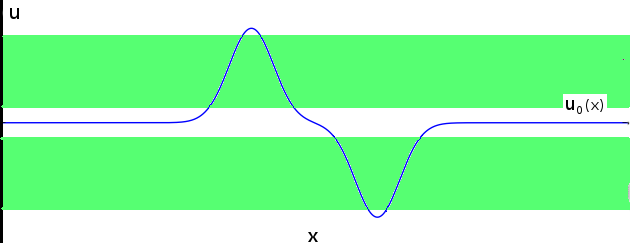
\includegraphics[height=3.3cm]{demo_theorem_1.png}
%        \caption{Illustration of $\mathcal{E}$ in theorem \ref{theorem: 1}, 
%                 the blue line shows $u_0(x)$. $\mathcal{E}$ is is colored green.}
%        \label{fig:demo_theorem_1}
%    \end{center}
%\end{figure}
%
%\noindent However, in realistic problems, generally $u$ has more than 1 dimensions.
%Besides, the primal model is a discretized PDE. It will be hard, if not impossible, 
%to give a close-form expression for $\mathcal{E}$. So we have to 
%determine $\mathcal{E}$ numerically. 




